\documentclass[../Dore_vision.tex]{subfiles}

\begin{document}

\section{Canto 01(1)}

\begin{figure}[ht]
\centering
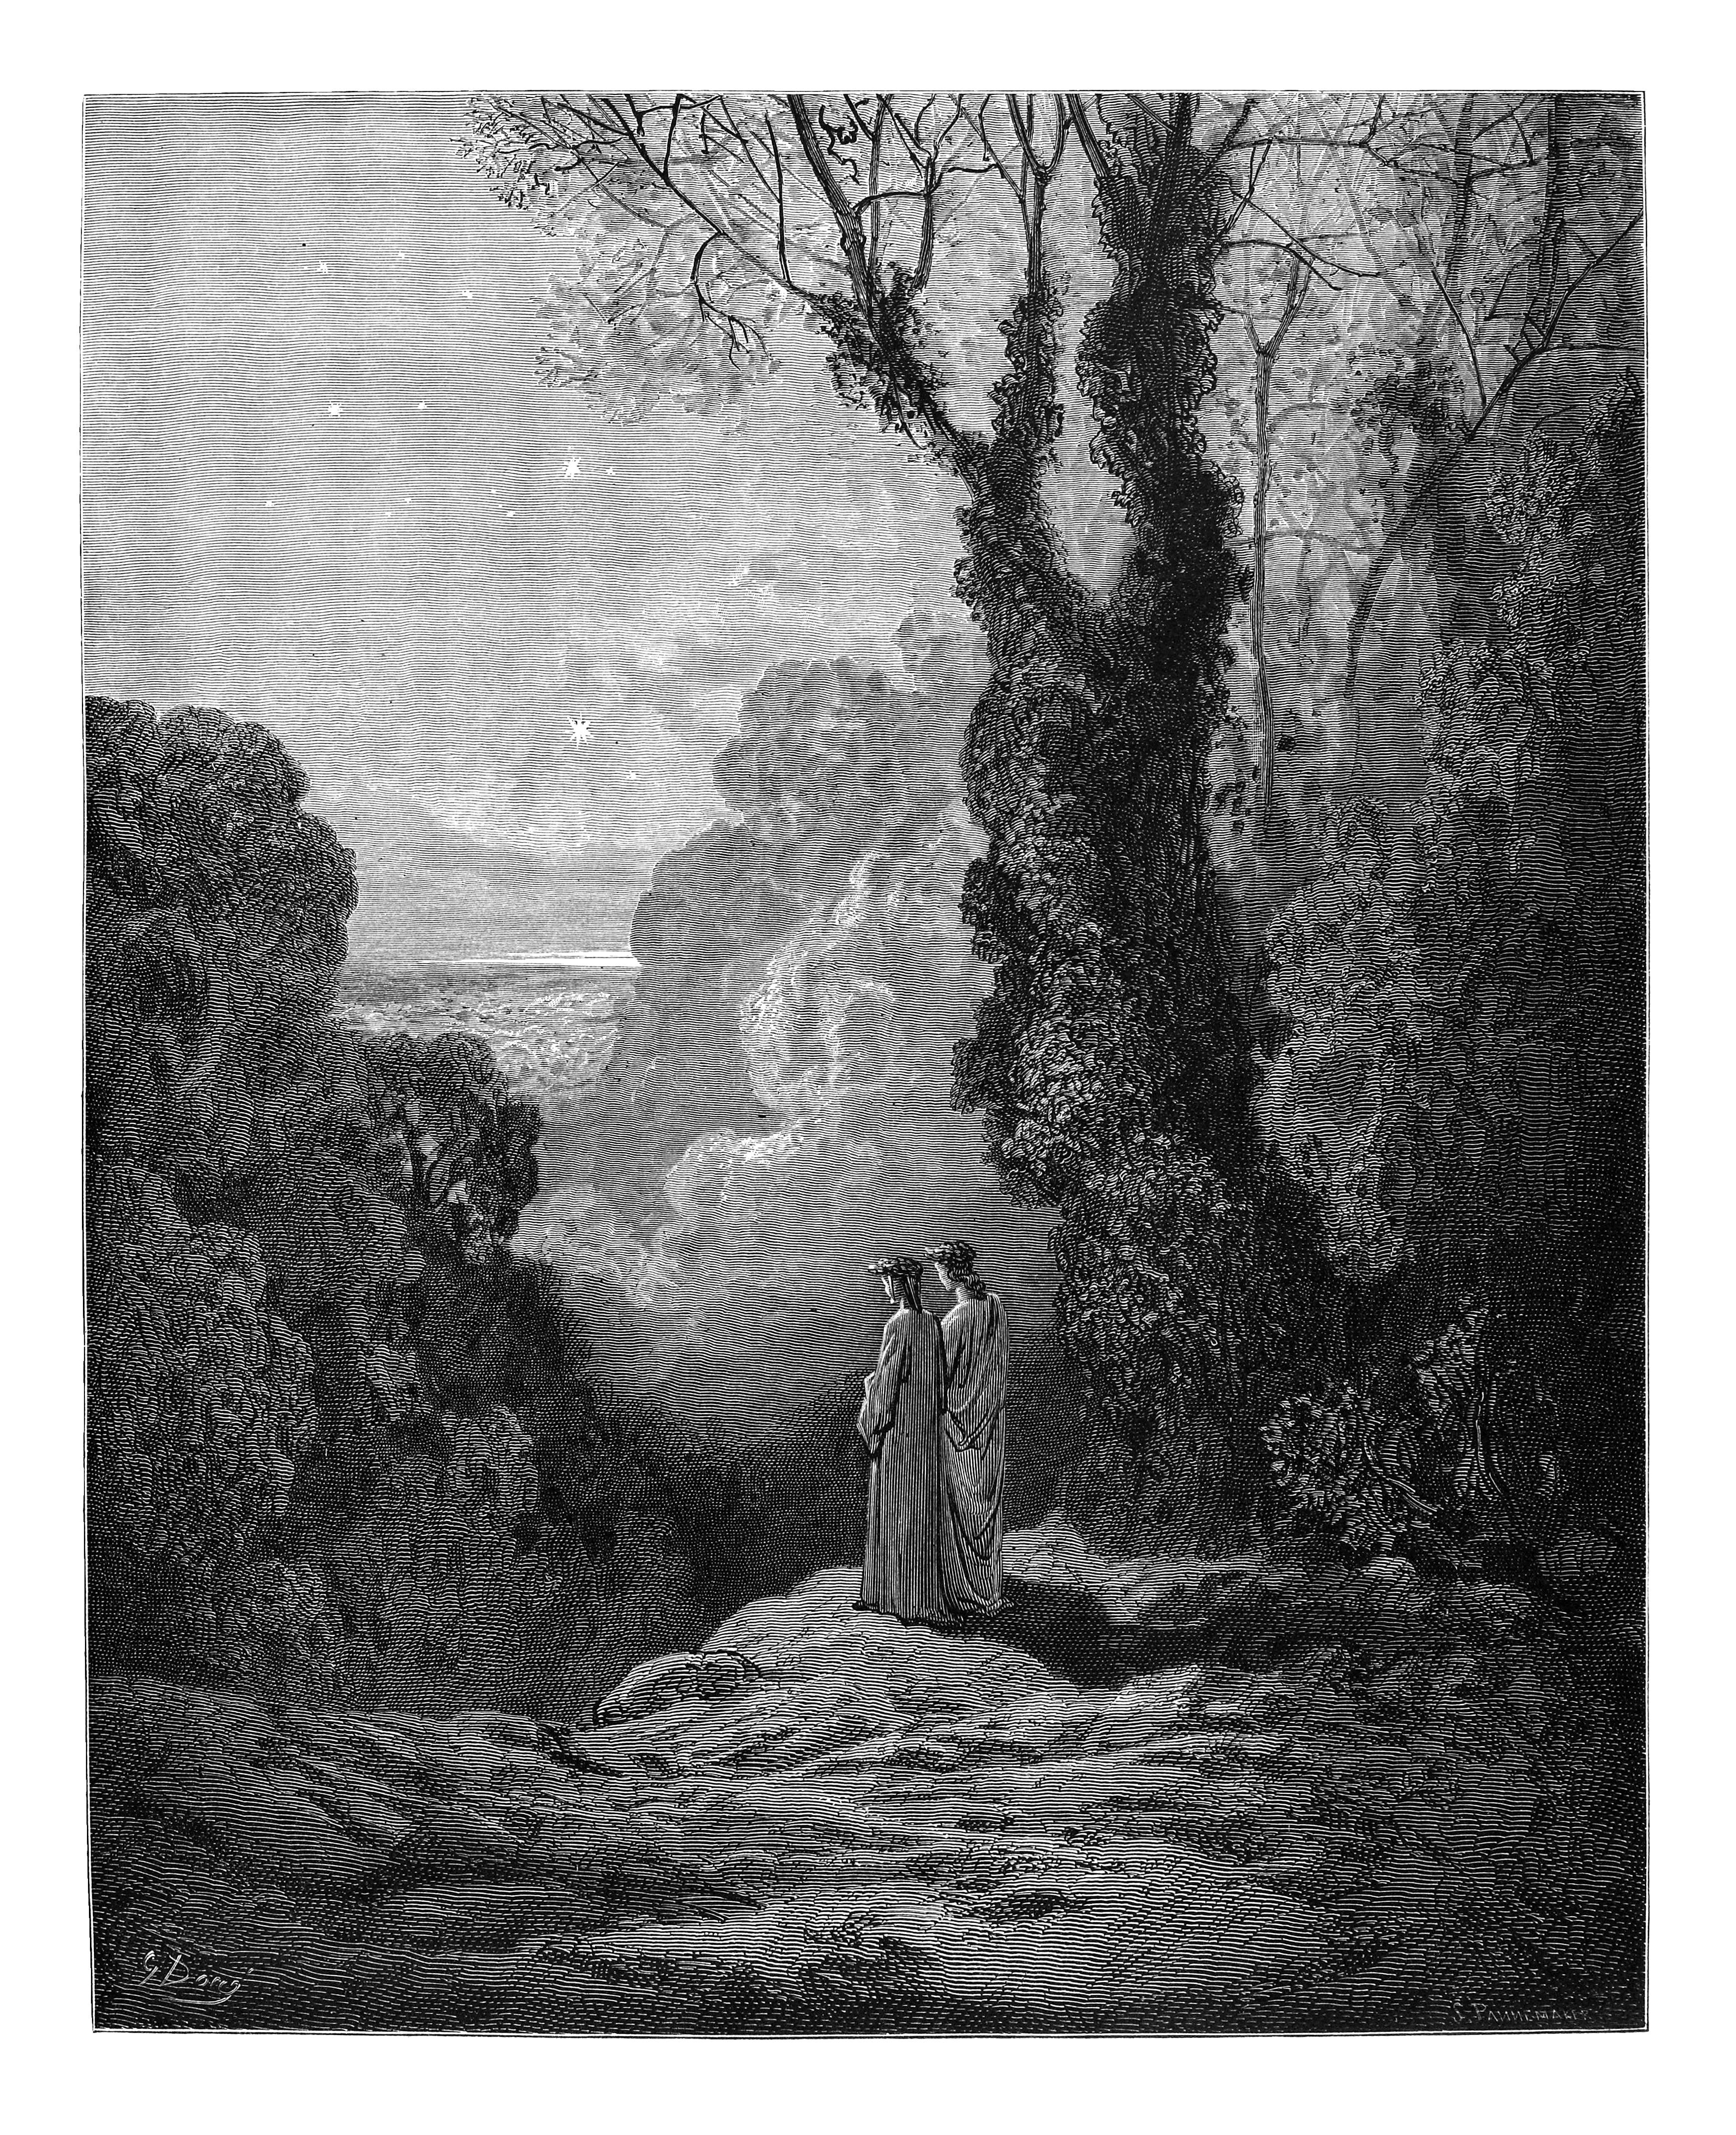
\includegraphics[height=\figsize]{illustrations/book_2/V02, c01(1).jpg}
\end{figure}

\begin{center}
\begin{minipage}{0.8\linewidth}
\textit{\\
"...vidi quattro stelle\\non viste mai fuor ch’a la prima gente."} \\
—V02, c01(1) \\~\\
\textit{"...I saw\\Four stars ne'er seen before save by the ken\\Of our first parents. …"} \\
—B02, c01(1)
\end{minipage}
\end{center}

\newpage

\section{Canto 01(2)}

\begin{figure}[ht]
\centering
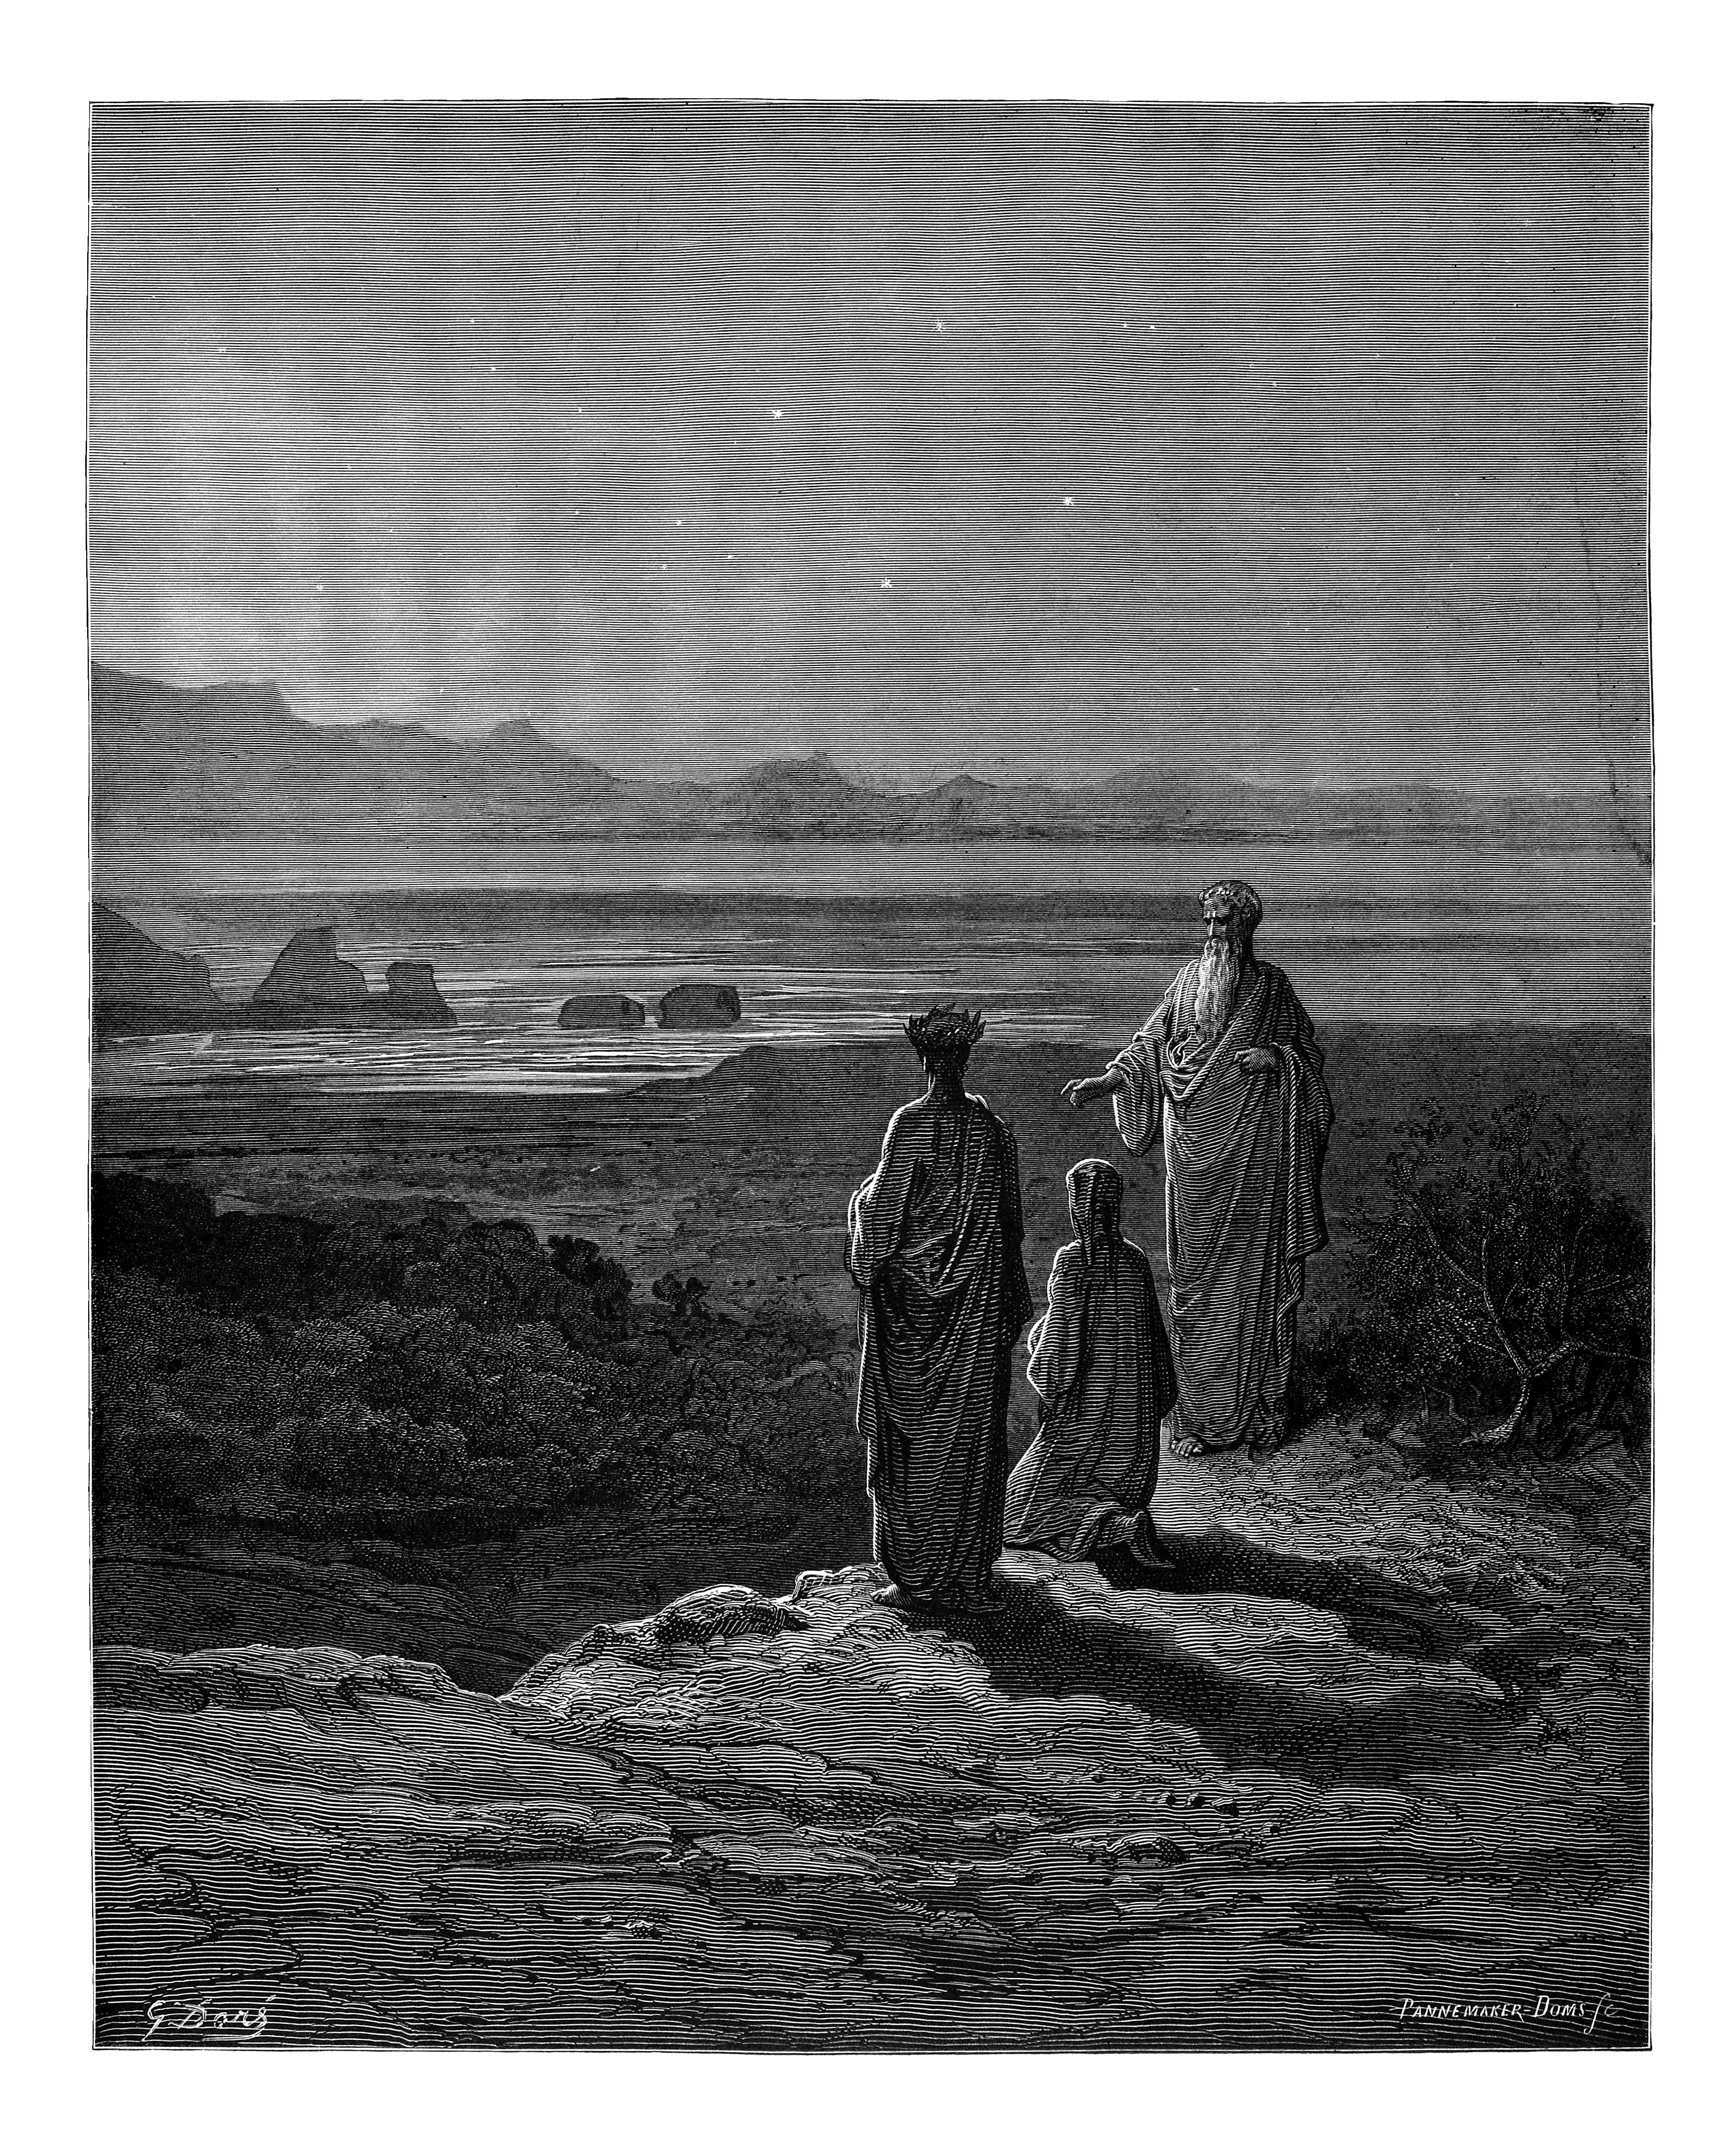
\includegraphics[height=\figsize]{illustrations/book_2/V02, c01(2).jpg}
\end{figure}

\begin{center}
\begin{minipage}{0.8\linewidth}
\textit{\\
"vidi presso di me un veglio solo,"} \\
—V02, c01(2) \\~\\
\textit{"I saw an old man standing by my side\\Alone, ..."} \\
—B02, c01(2)
\end{minipage}
\end{center}

\newpage

\section{Canto 02(1)}

\begin{figure}[ht]
\centering
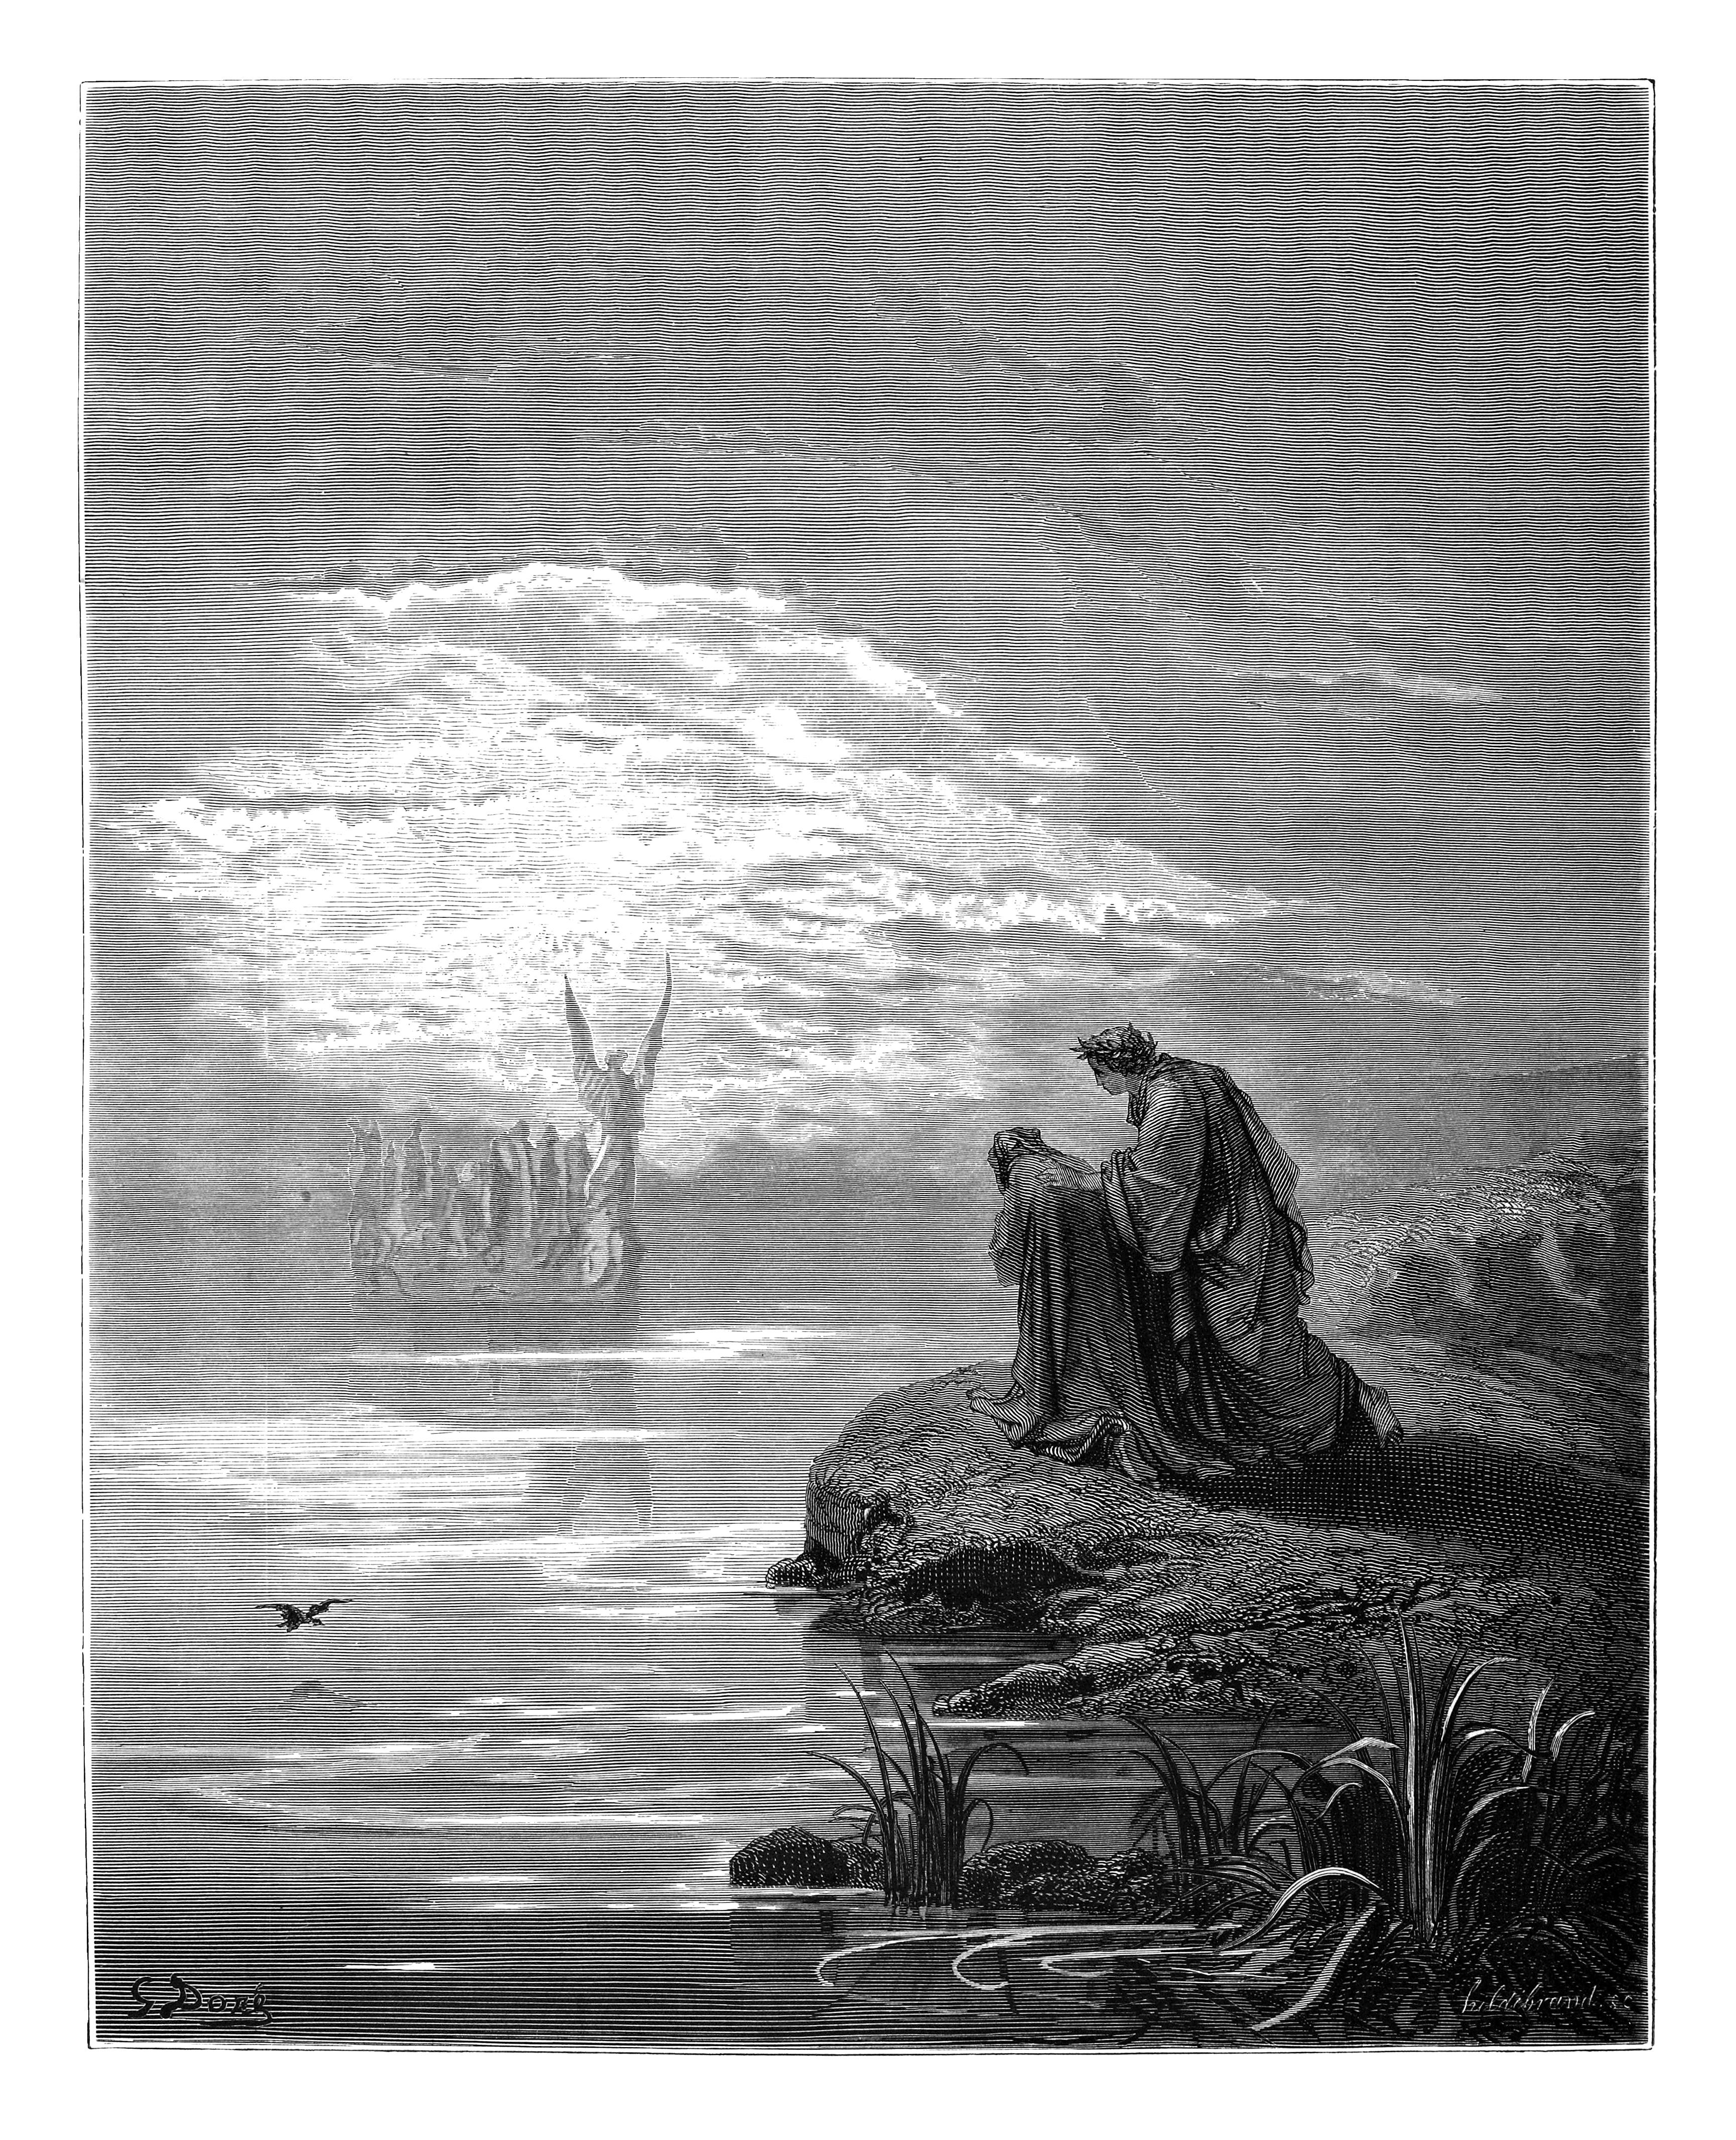
\includegraphics[height=\figsize]{illustrations/book_2/V02, c02(1).jpg}
\end{figure}

\begin{center}
\begin{minipage}{0.8\linewidth}
\textit{\\
"...come più e più verso noi venne\\l’uccel divino, più chiaro appariva:"} \\
—V02, c02(1) \\~\\
\textit{"As more and more toward us came, more bright\\Appear'd the bird of God, …"} \\
—B02, c02(1)
\end{minipage}
\end{center}

\newpage

\section{Canto 02(2)}

\begin{figure}[ht]
\centering
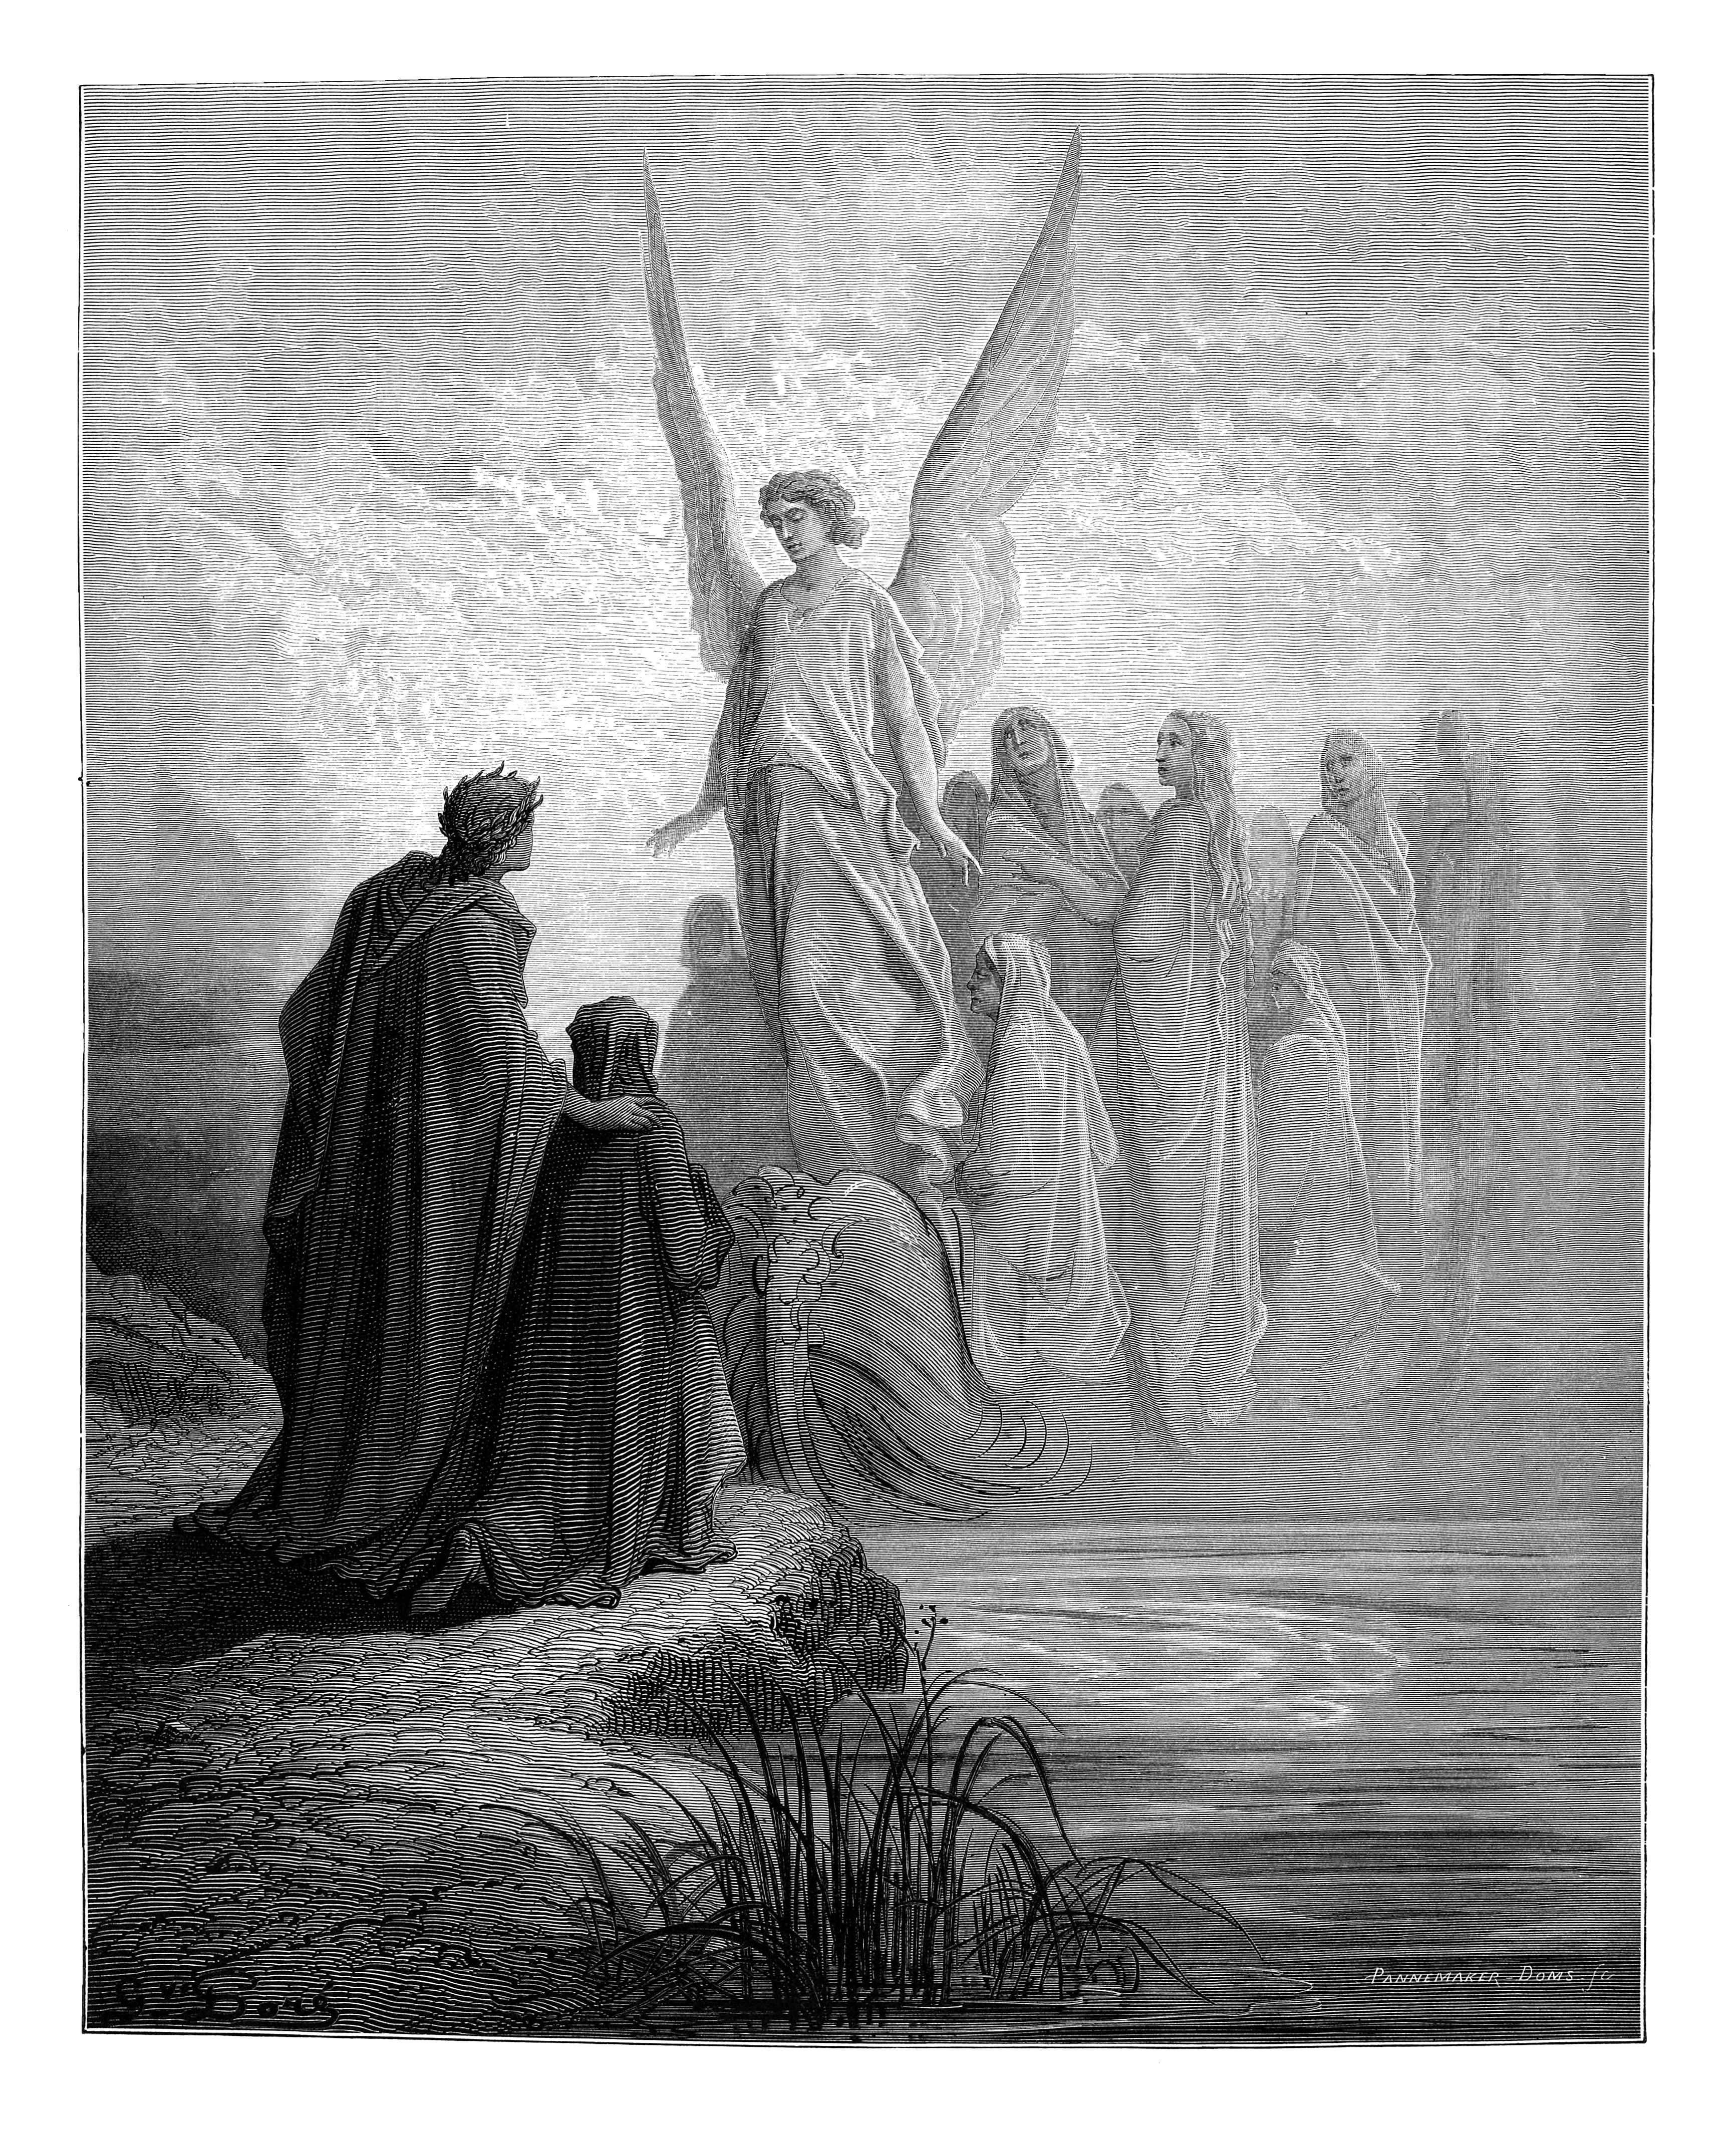
\includegraphics[height=\figsize]{illustrations/book_2/V02, c02(2).jpg}
\end{figure}

\begin{center}
\begin{minipage}{0.8\linewidth}
\textit{\\
"«In exitu Israel de Aegypto»\\cantavan tutti insieme ad una voce"} \\
—V02, c02(2) \\~\\
\textit{"\textquotesingle In Exitu Israel de Aegypto;\textquotesingle \\All with one voice together sang, …"} \\
—B02, c02(2)
\end{minipage}
\end{center}

\newpage

\section{Canto 03}

\begin{figure}[ht]
\centering
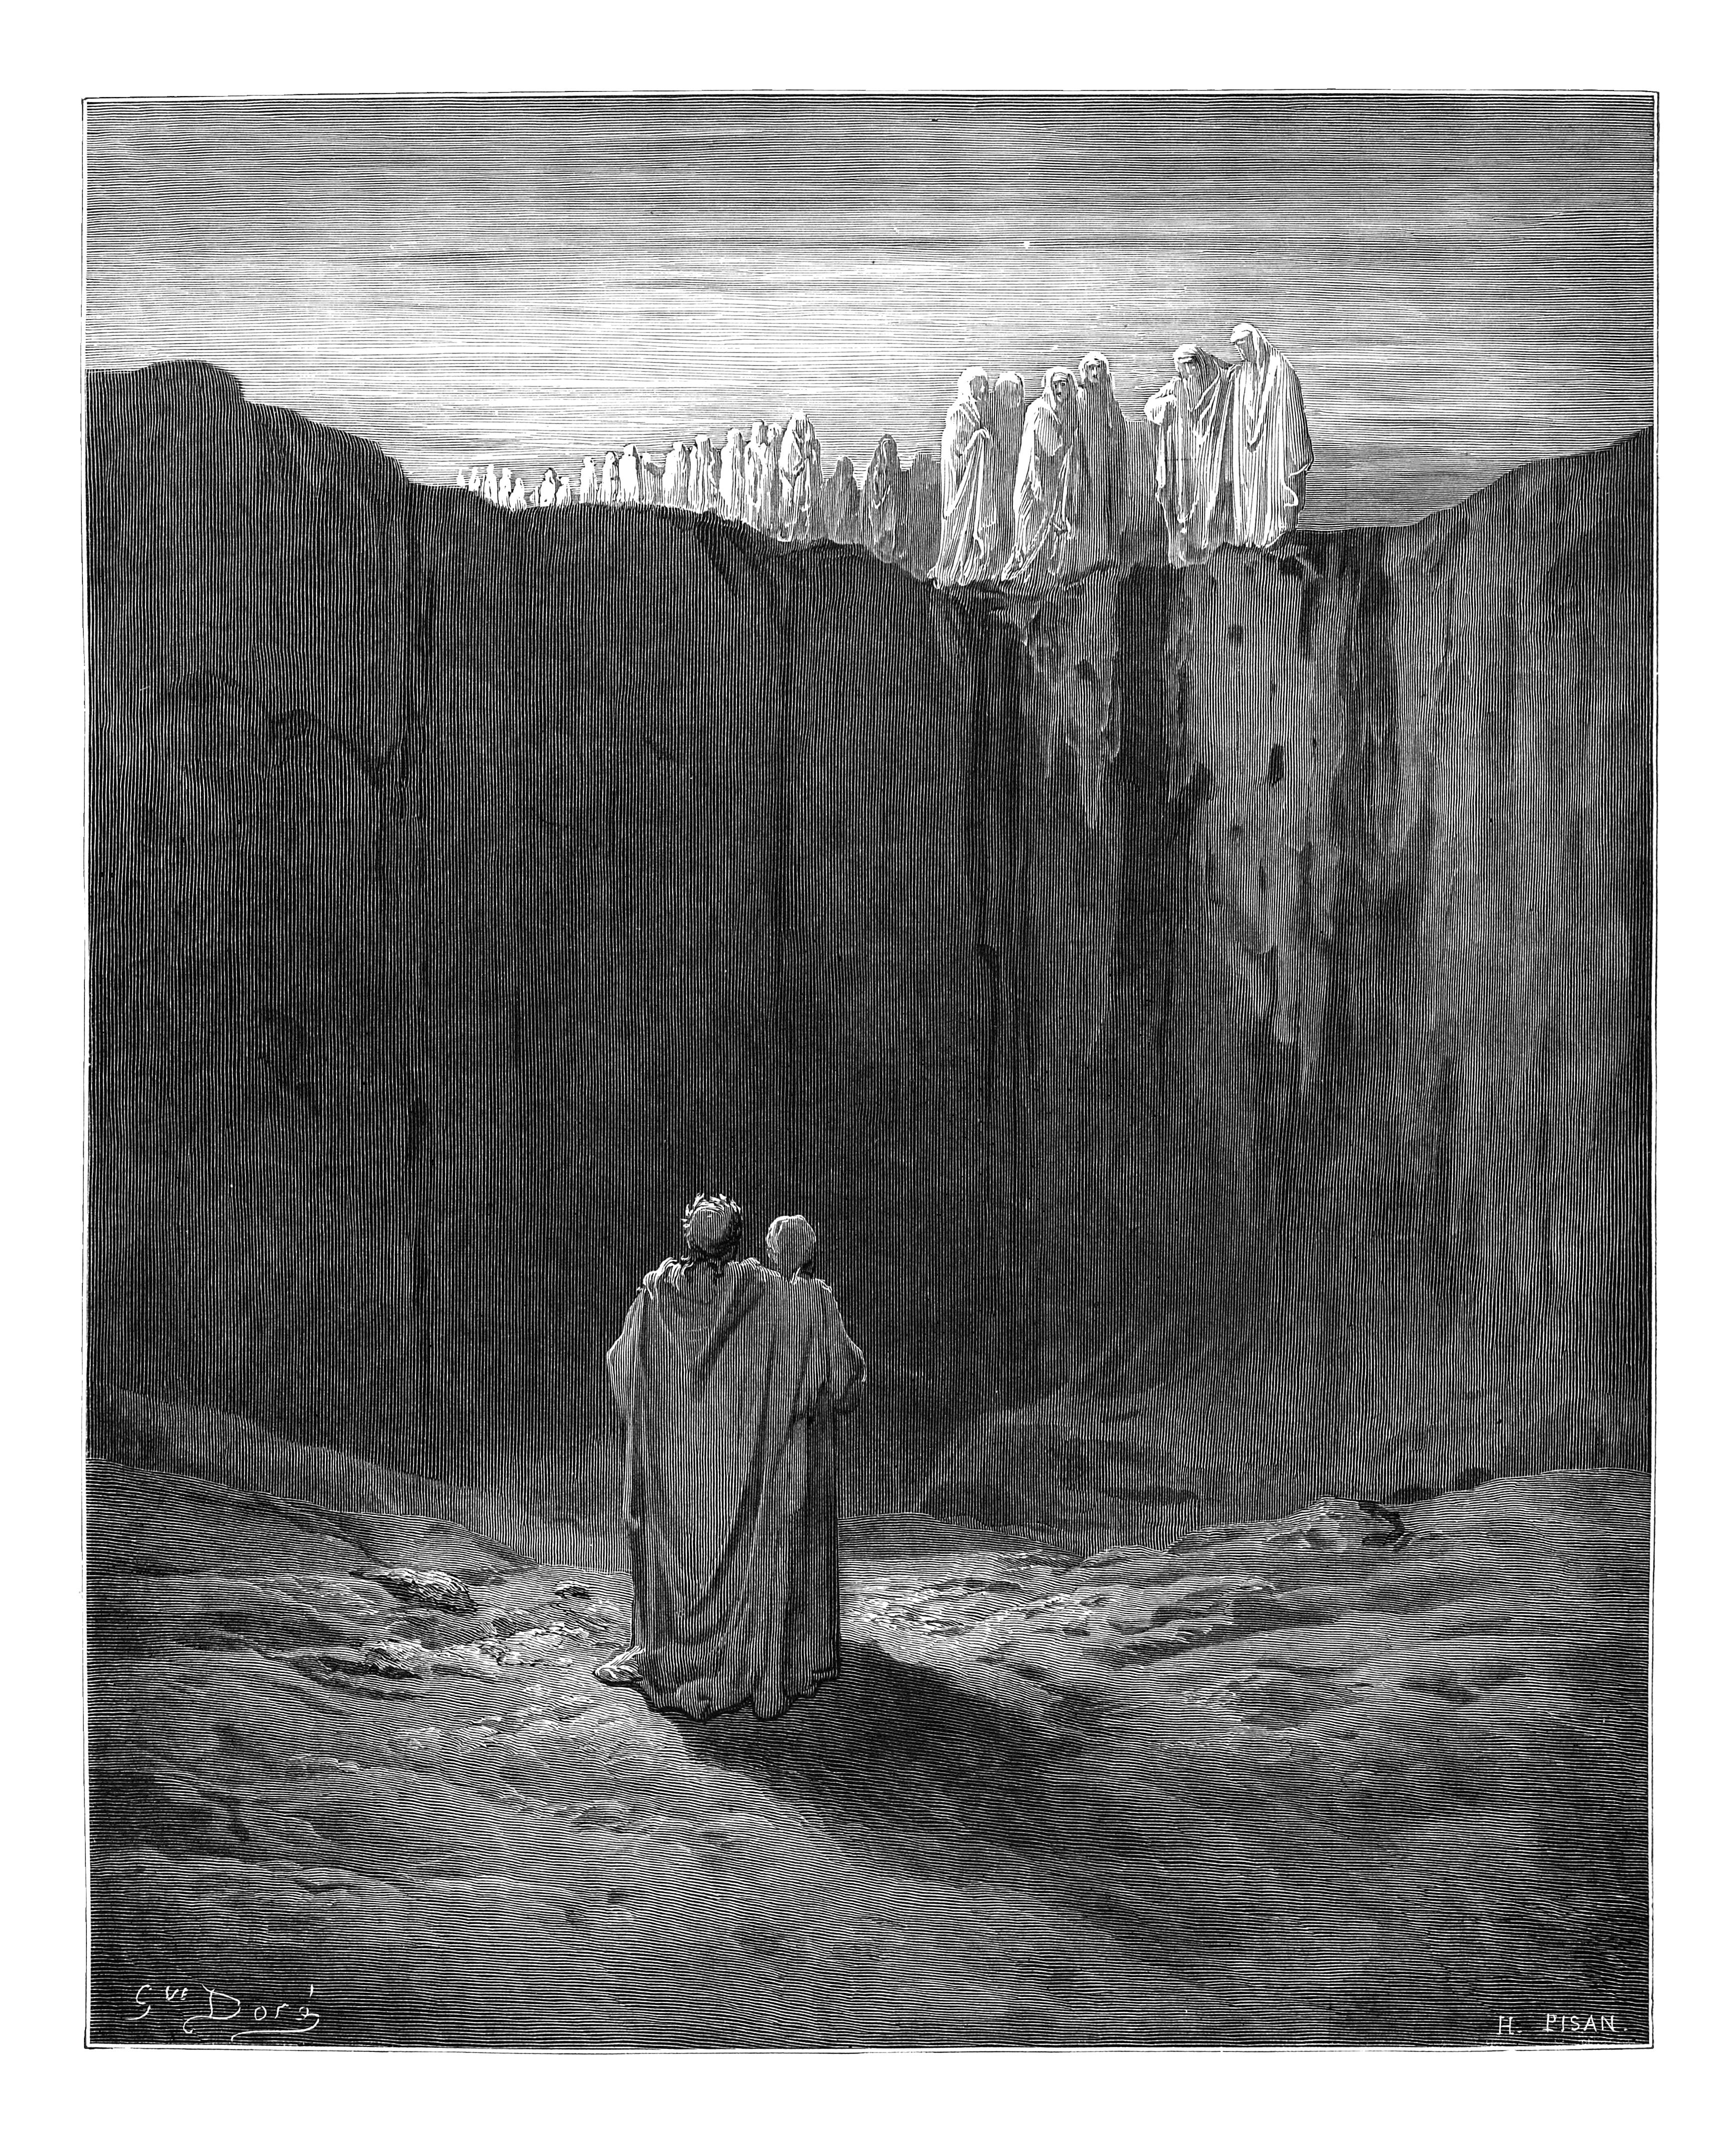
\includegraphics[height=\figsize]{illustrations/book_2/V02, c03.jpg}
\end{figure}

\begin{center}
\begin{minipage}{0.8\linewidth}
\textit{\\
"da man sinistra m’appar\`{\i} una gente\\d’anime, che movieno i piè ver’ noi,"} \\
—V02, c03 \\~\\
\textit{"...I gaz'd upward round the stony height,\\Of spirits, that toward us mov'd their steps,"} \\
—B02, c03
\end{minipage}
\end{center}

\newpage

\section{Canto 04(1)}

\begin{figure}[ht]
\centering
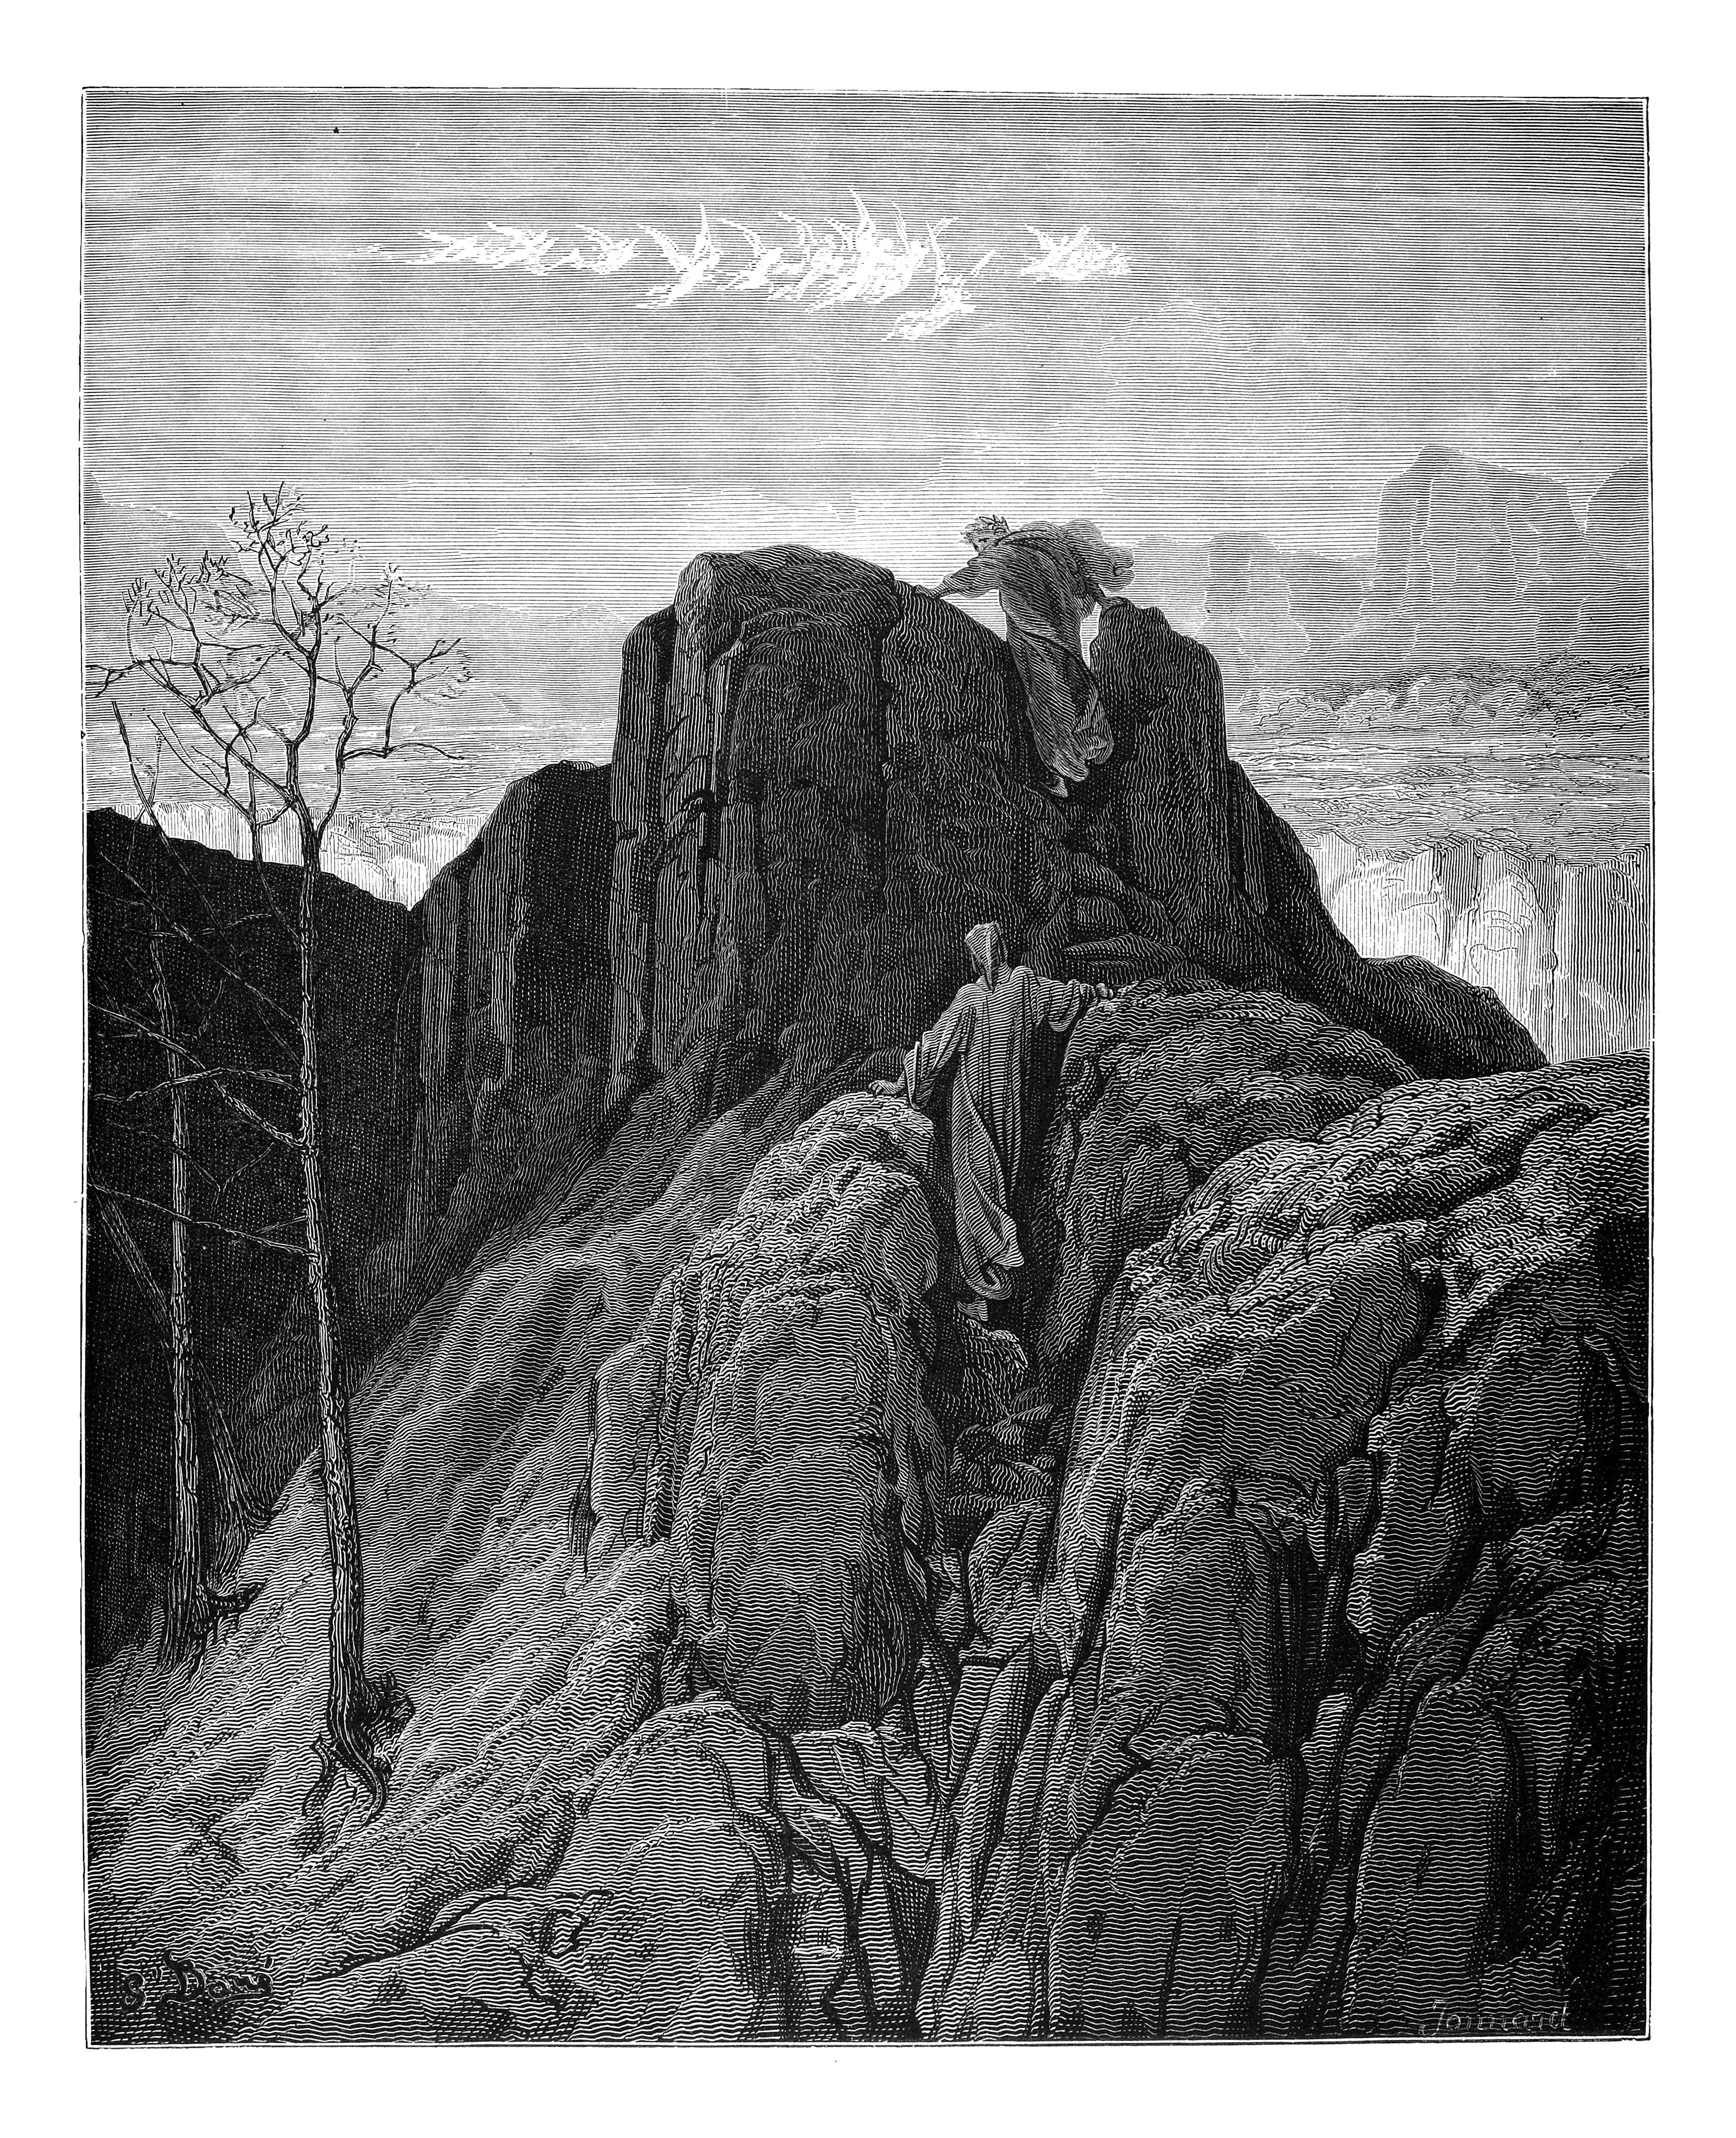
\includegraphics[height=\figsize]{illustrations/book_2/V02, c04(1).jpg}
\end{figure}

\begin{center}
\begin{minipage}{0.8\linewidth}
\textit{\\
"Noi salavam per entro ’l sasso rotto,"} \\
—V02, c04(1) \\~\\
\textit{"We through the broken rock ascended, …"} \\
—B02, c04(1)
\end{minipage}
\end{center}

\newpage

\section{Canto 04(2)}

\begin{figure}[ht]
\centering
\includegraphics[height=\figsize]{illustrations/book_2/V02, c04(2).jpg}
\end{figure}

\begin{center}
\begin{minipage}{0.8\linewidth}
\textit{\\
"...ivi eran persone\\che si stavano a l’ombra dietro al sasso\\come l’uom per negghienza a star si pone."} \\
—V02, c04(2) \\~\\
\textit{"...there were some, who in the shady place\\Behind the rock were standing, as a man\\Thru' idleness might stand. …"} \\
—B02, c04(2)
\end{minipage}
\end{center}

\newpage

\section{Canto 05(1)}

\begin{figure}[ht]
\centering
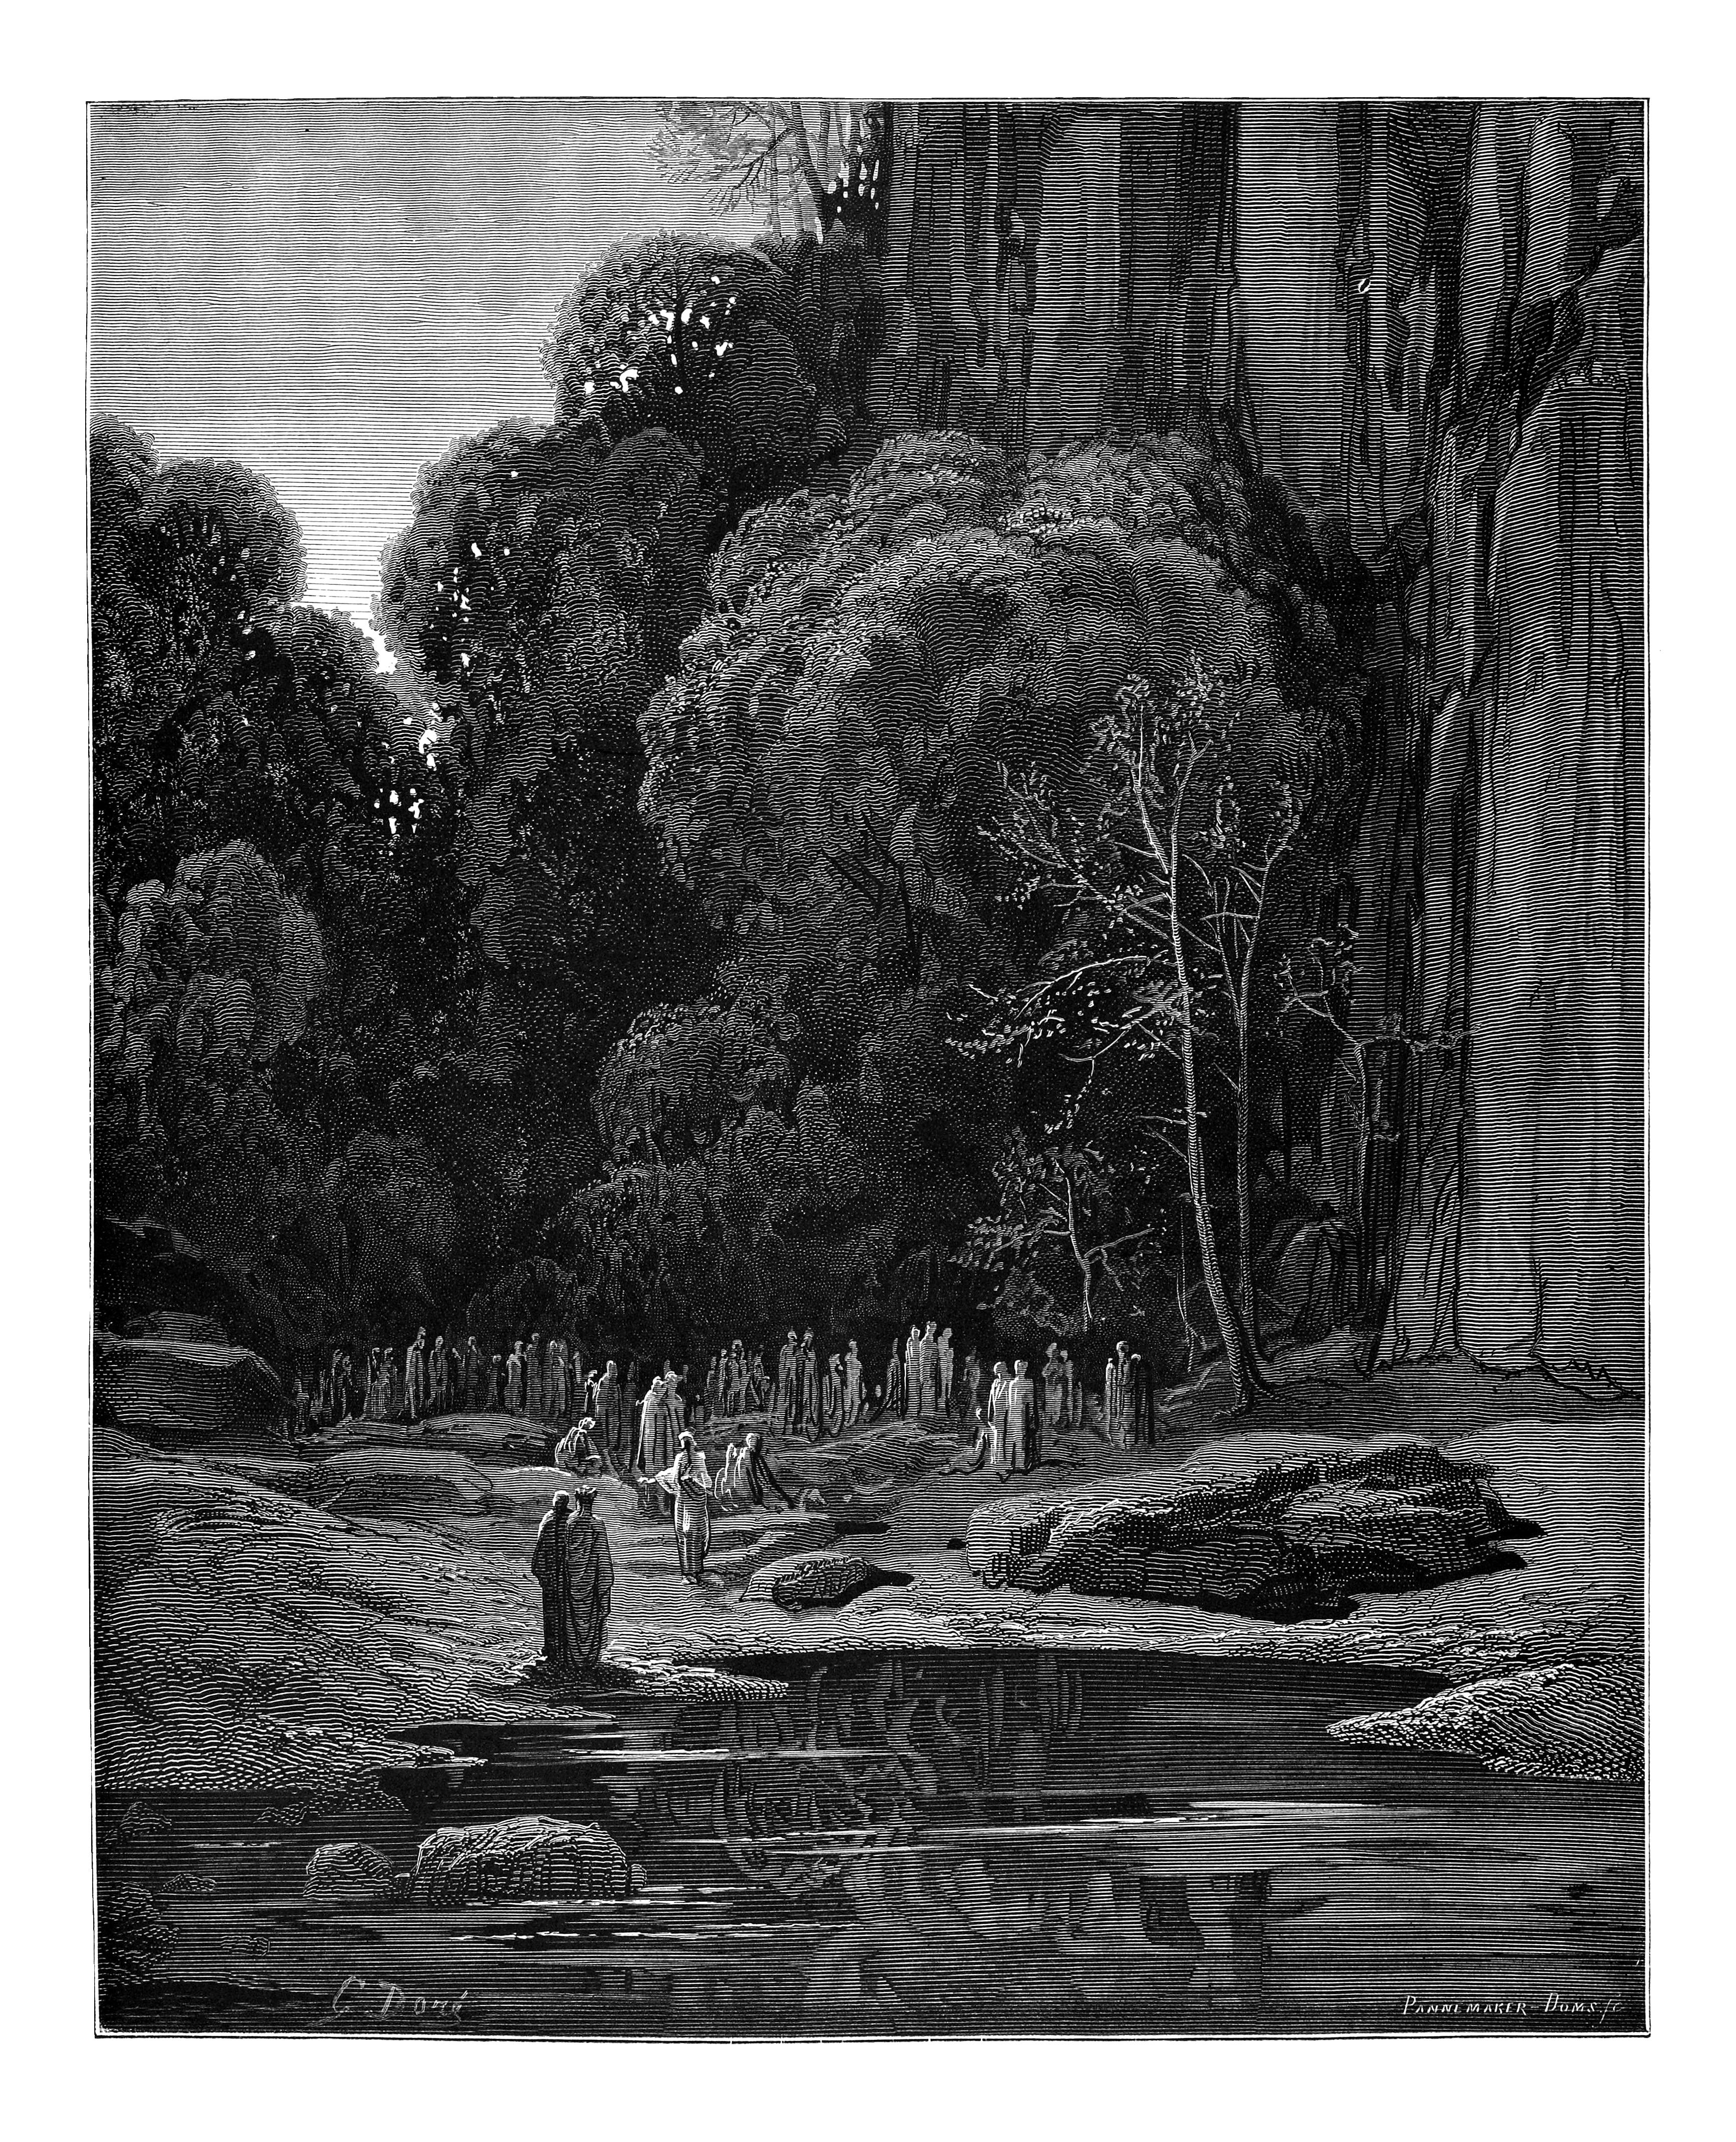
\includegraphics[height=\figsize]{illustrations/book_2/V02, c05(1).jpg}
\end{figure}

\begin{center}
\begin{minipage}{0.8\linewidth}
\textit{\\
"...per la costa di traverso\\venivan genti innanzi a noi un poco,\\cantando «Miserere»…"} \\
—V02, c05(1) \\~\\
\textit{"...traverse along the hill there came,\\A little way before us, some who sang\\The \textquotesingle Miserere\textquotesingle…"} \\
—B02, c05(1)
\end{minipage}
\end{center}

\newpage

\section{Canto 05(2)}

\begin{figure}[ht]
\centering
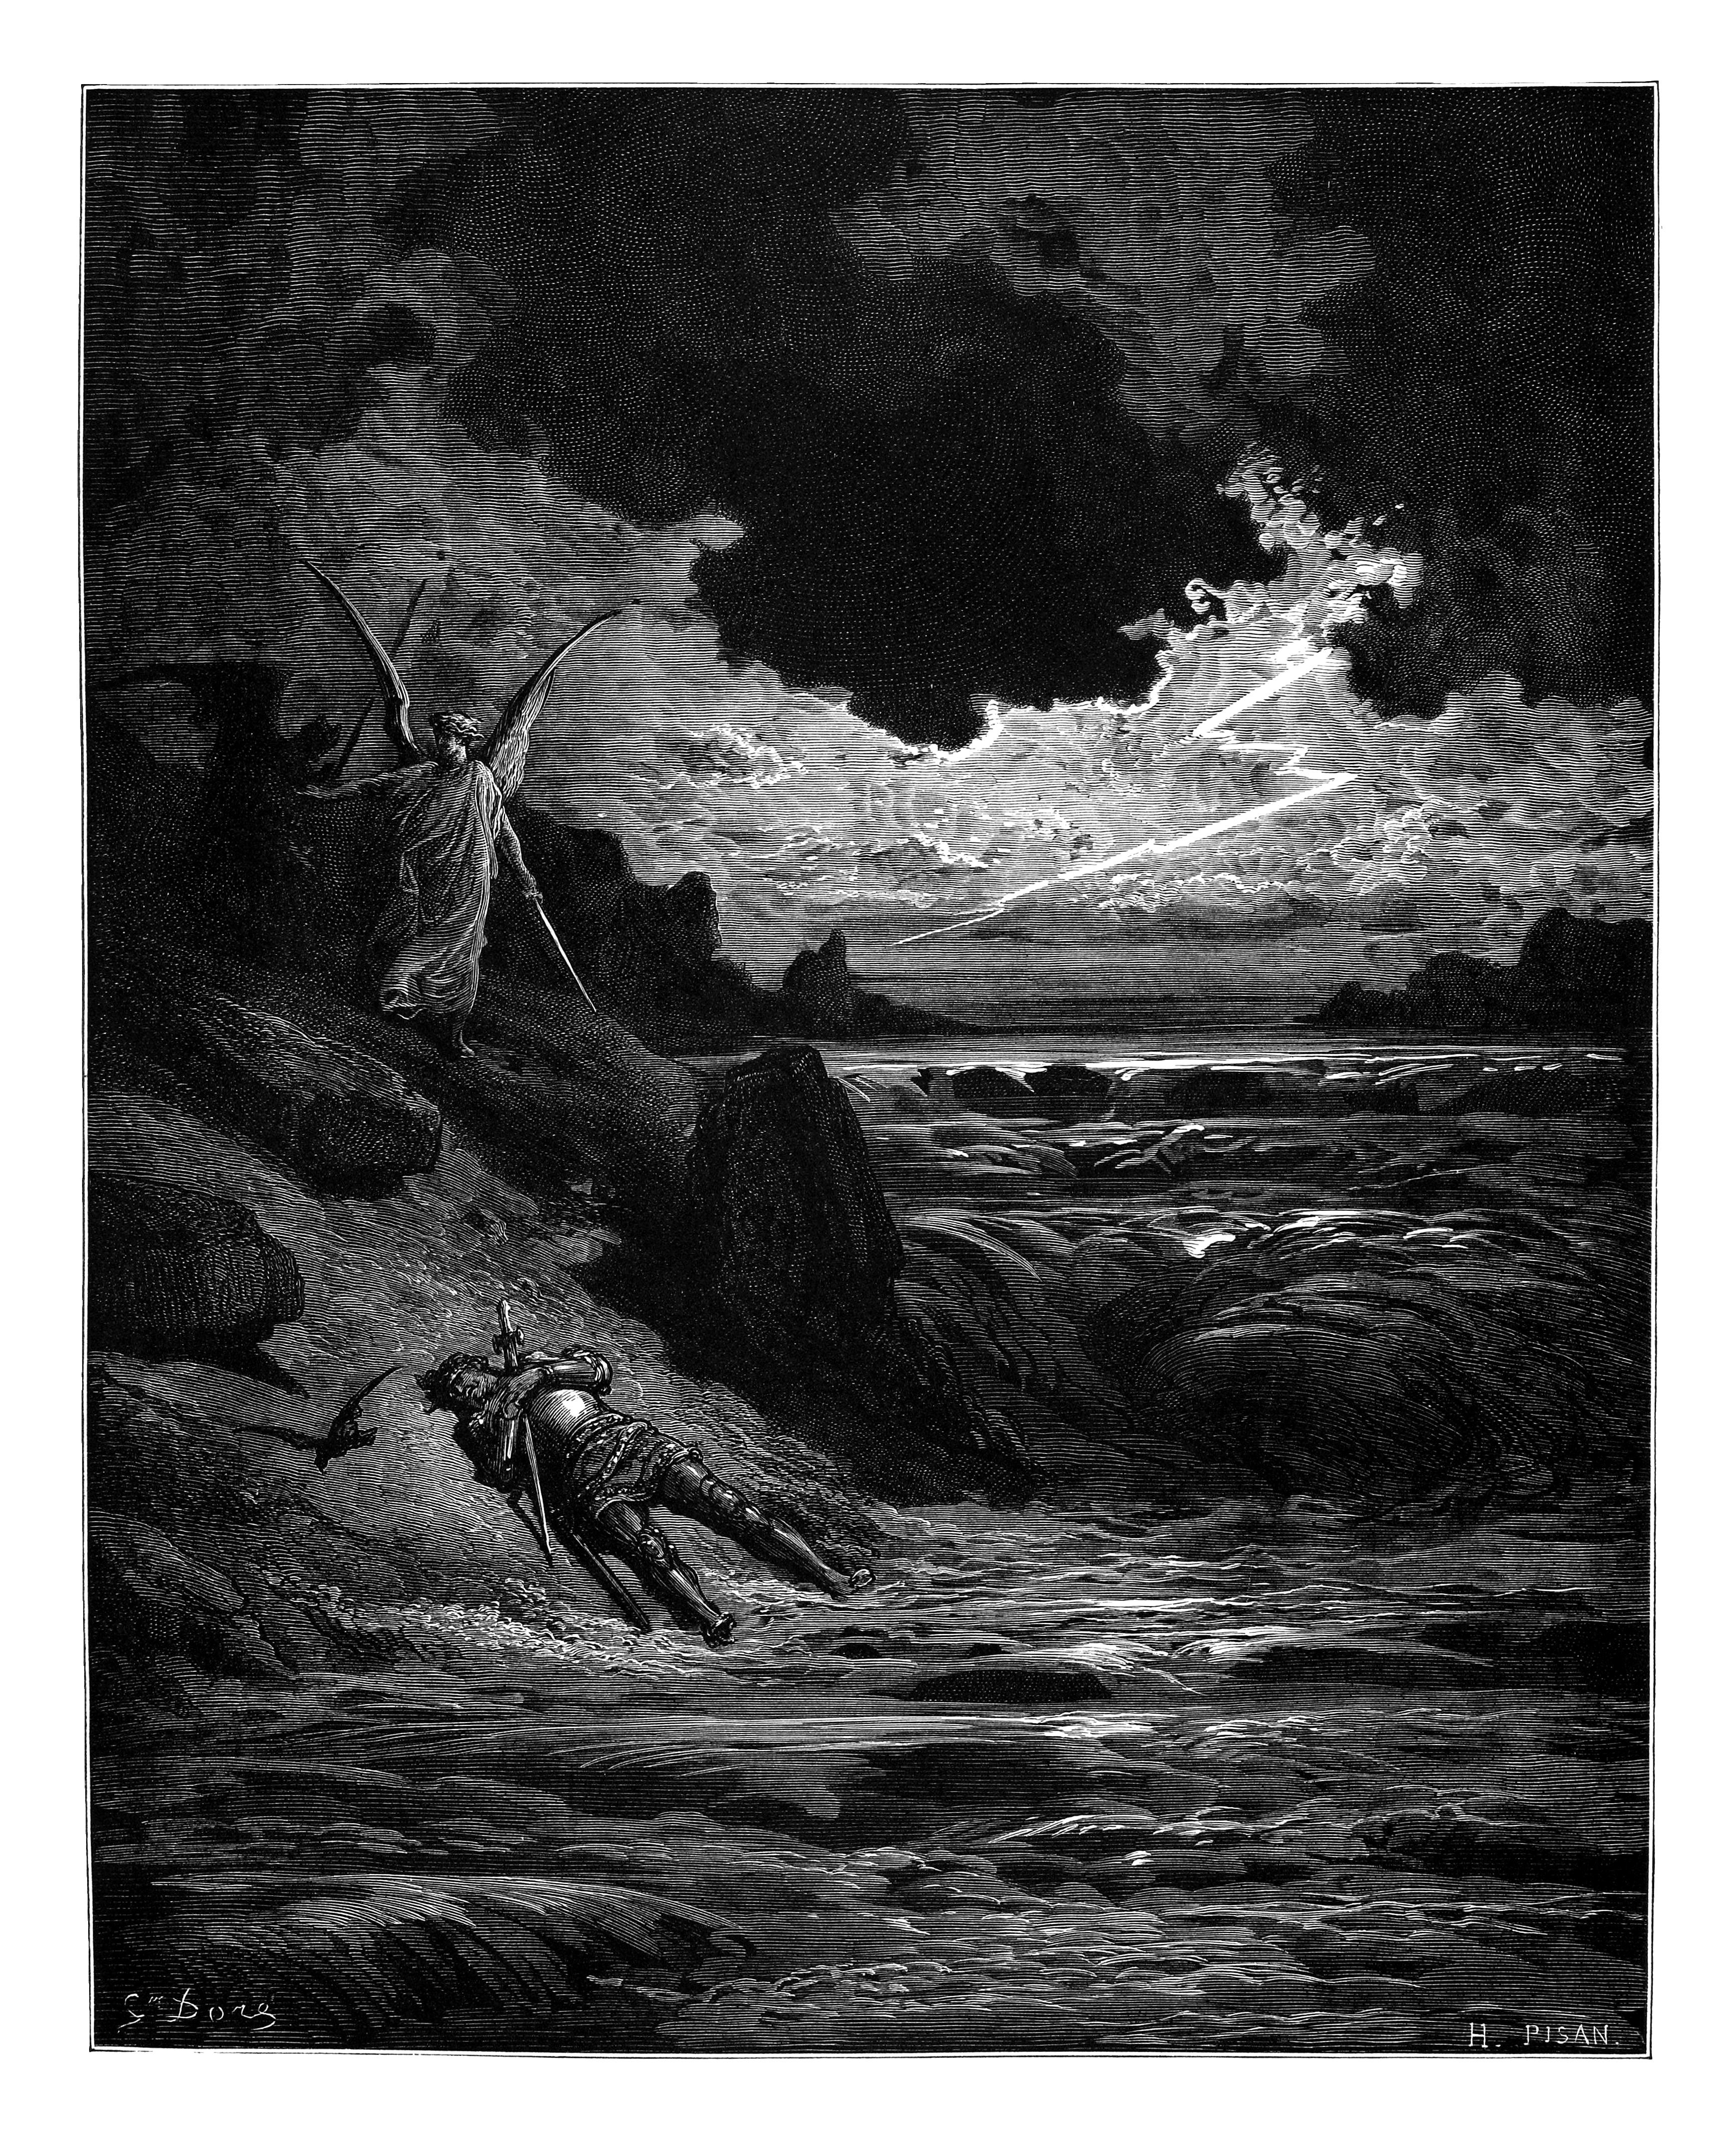
\includegraphics[height=\figsize]{illustrations/book_2/V02, c05(2).jpg}
\end{figure}

\begin{center}
\begin{minipage}{0.8\linewidth}
\textit{\\
"Lo corpo mio gelato in su la foce\\trov\`o l’Archian rubesto; …"} \\
—V02, c05(2) \\~\\
\textit{"...My stiffen'd frame\\Laid at his mouth the fell Archiano found,"} \\
—B02, c05(2)
\end{minipage}
\end{center}

\newpage

\section{Canto 05(3)}

\begin{figure}[ht]
\centering
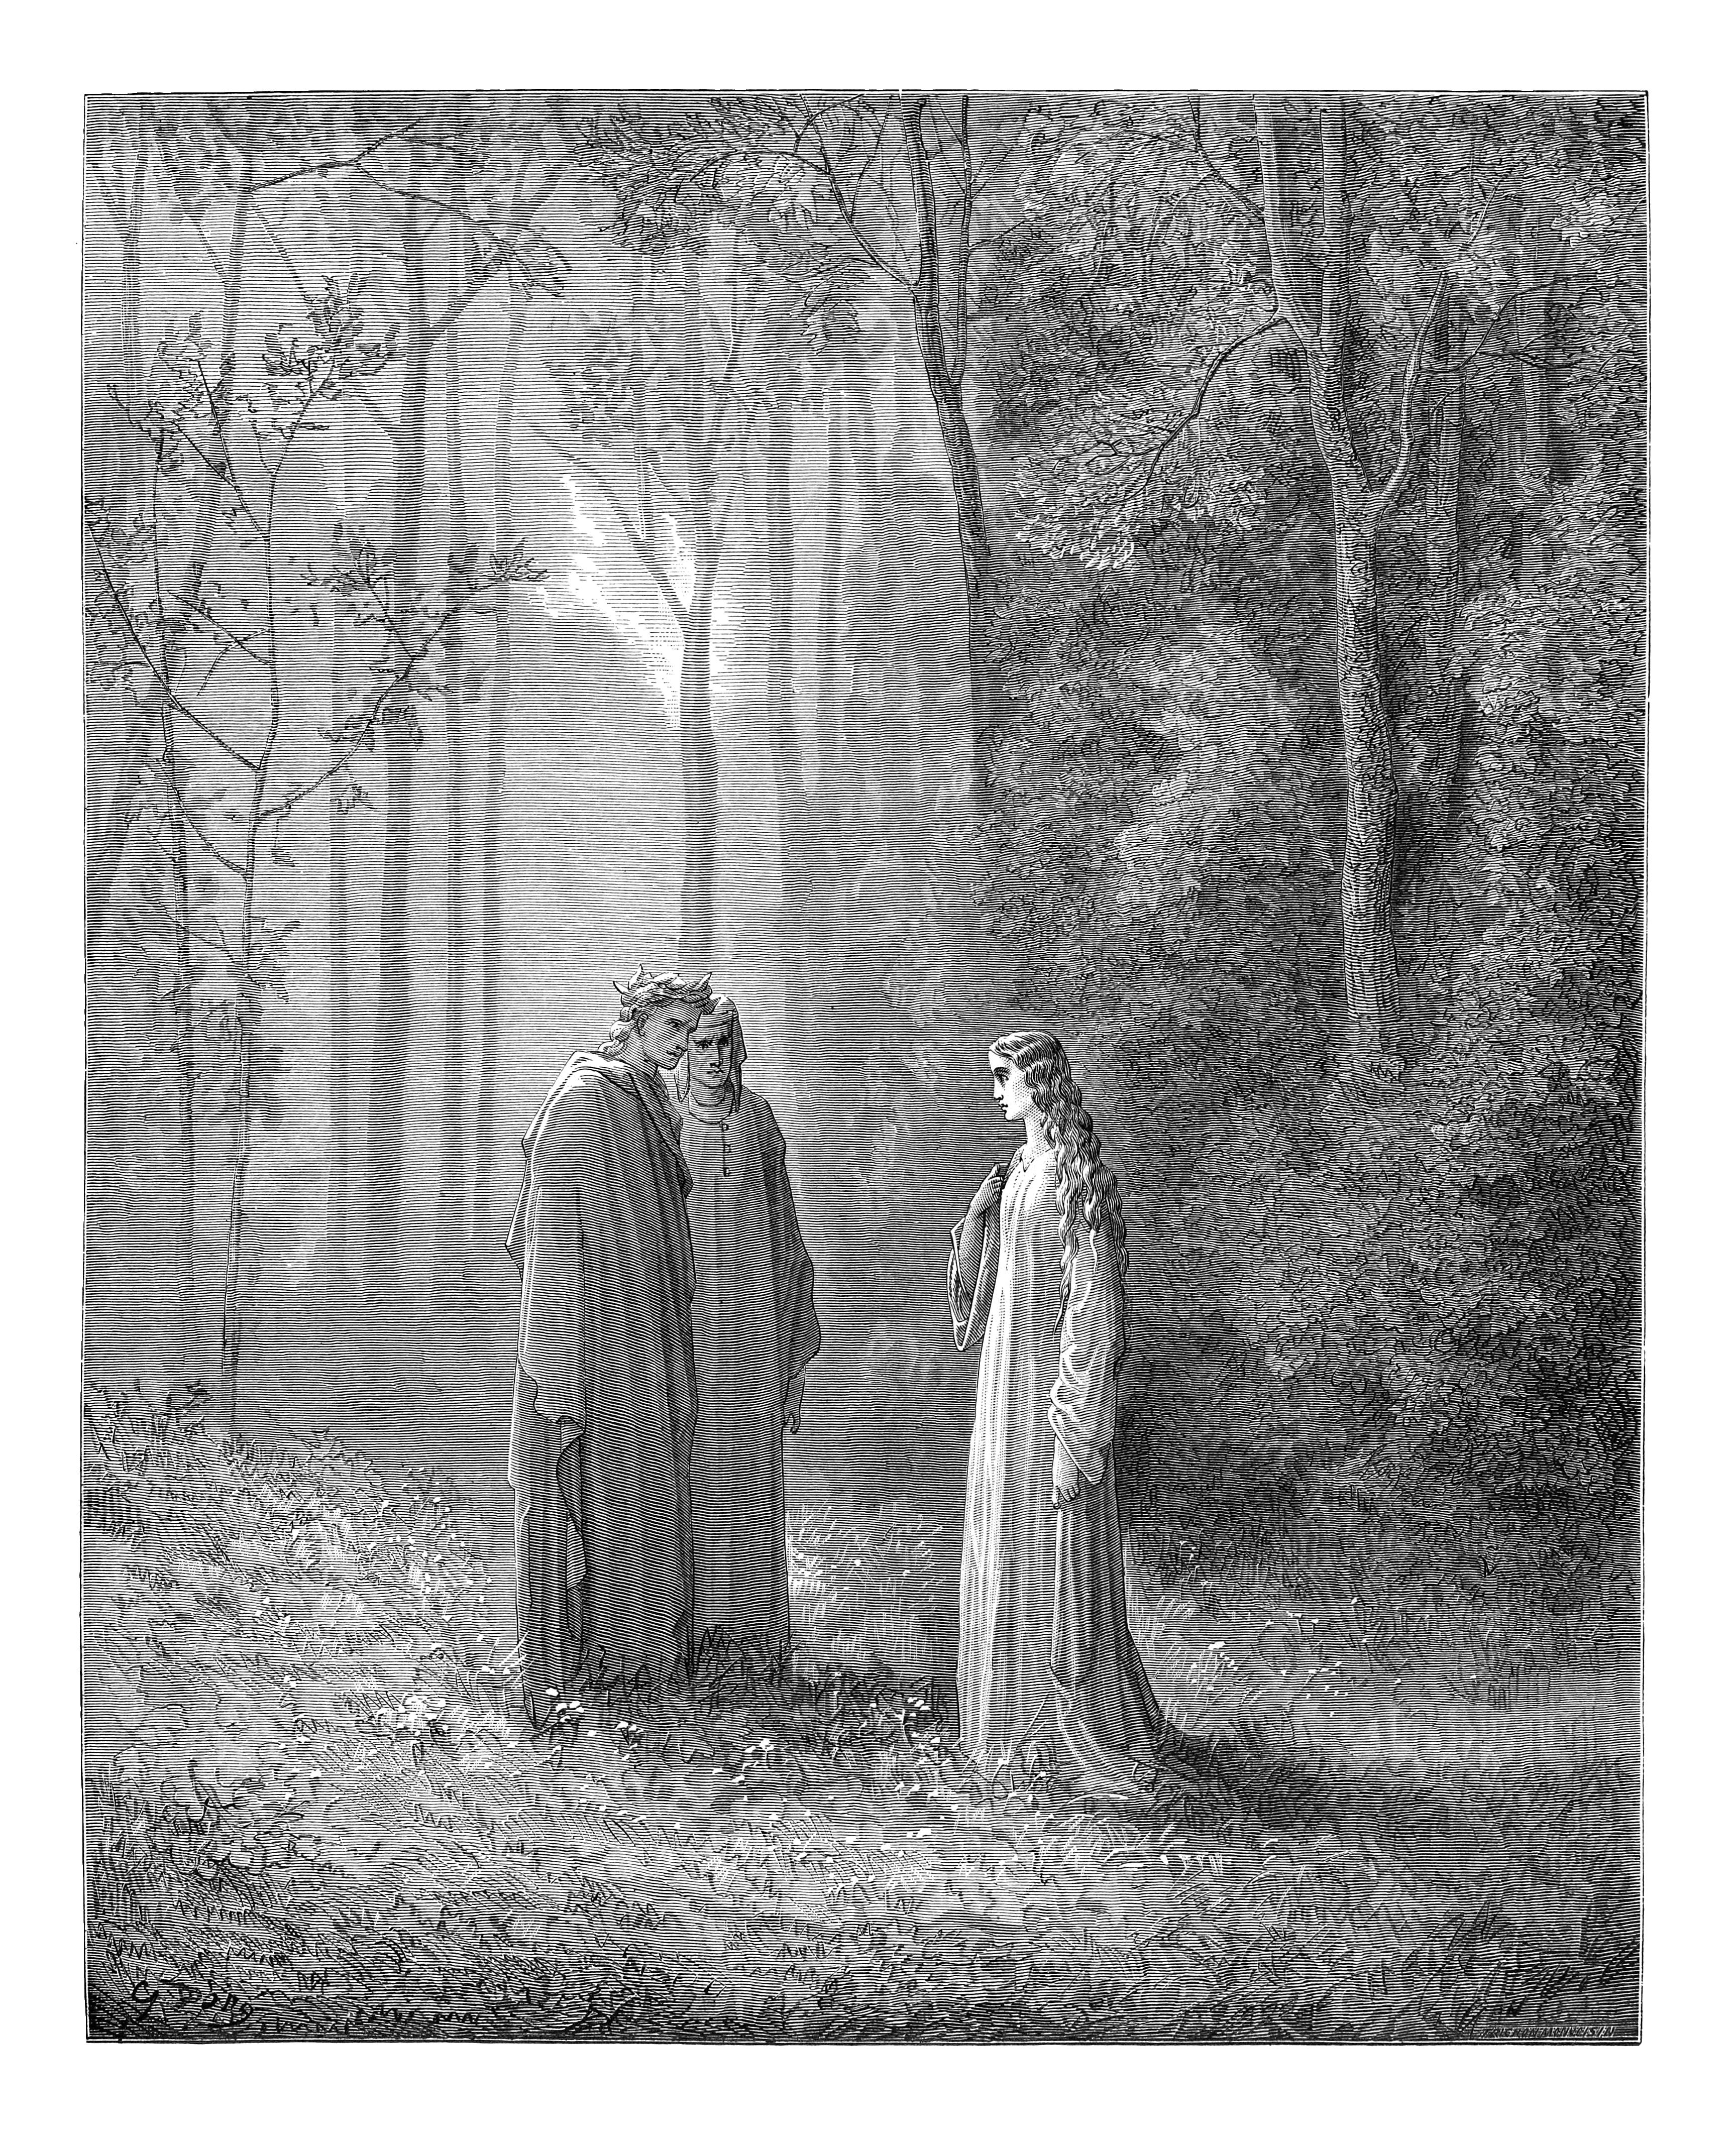
\includegraphics[height=\figsize]{illustrations/book_2/V02, c05(3).jpg}
\end{figure}

\begin{center}
\begin{minipage}{0.8\linewidth}
\textit{\\
"«ricorditi di me, che son la Pia:\\Siena mi fé, disfecemi Maremma:"} \\
—V02, c05(3) \\~\\
\textit{"...remember me.\\I once was Pia. Sienna gave me life,\\Maremma took it from me. …"} \\
—B02, c05(3)
\end{minipage}
\end{center}

\newpage

\section{Canto 07(1)}

\begin{figure}[ht]
\centering
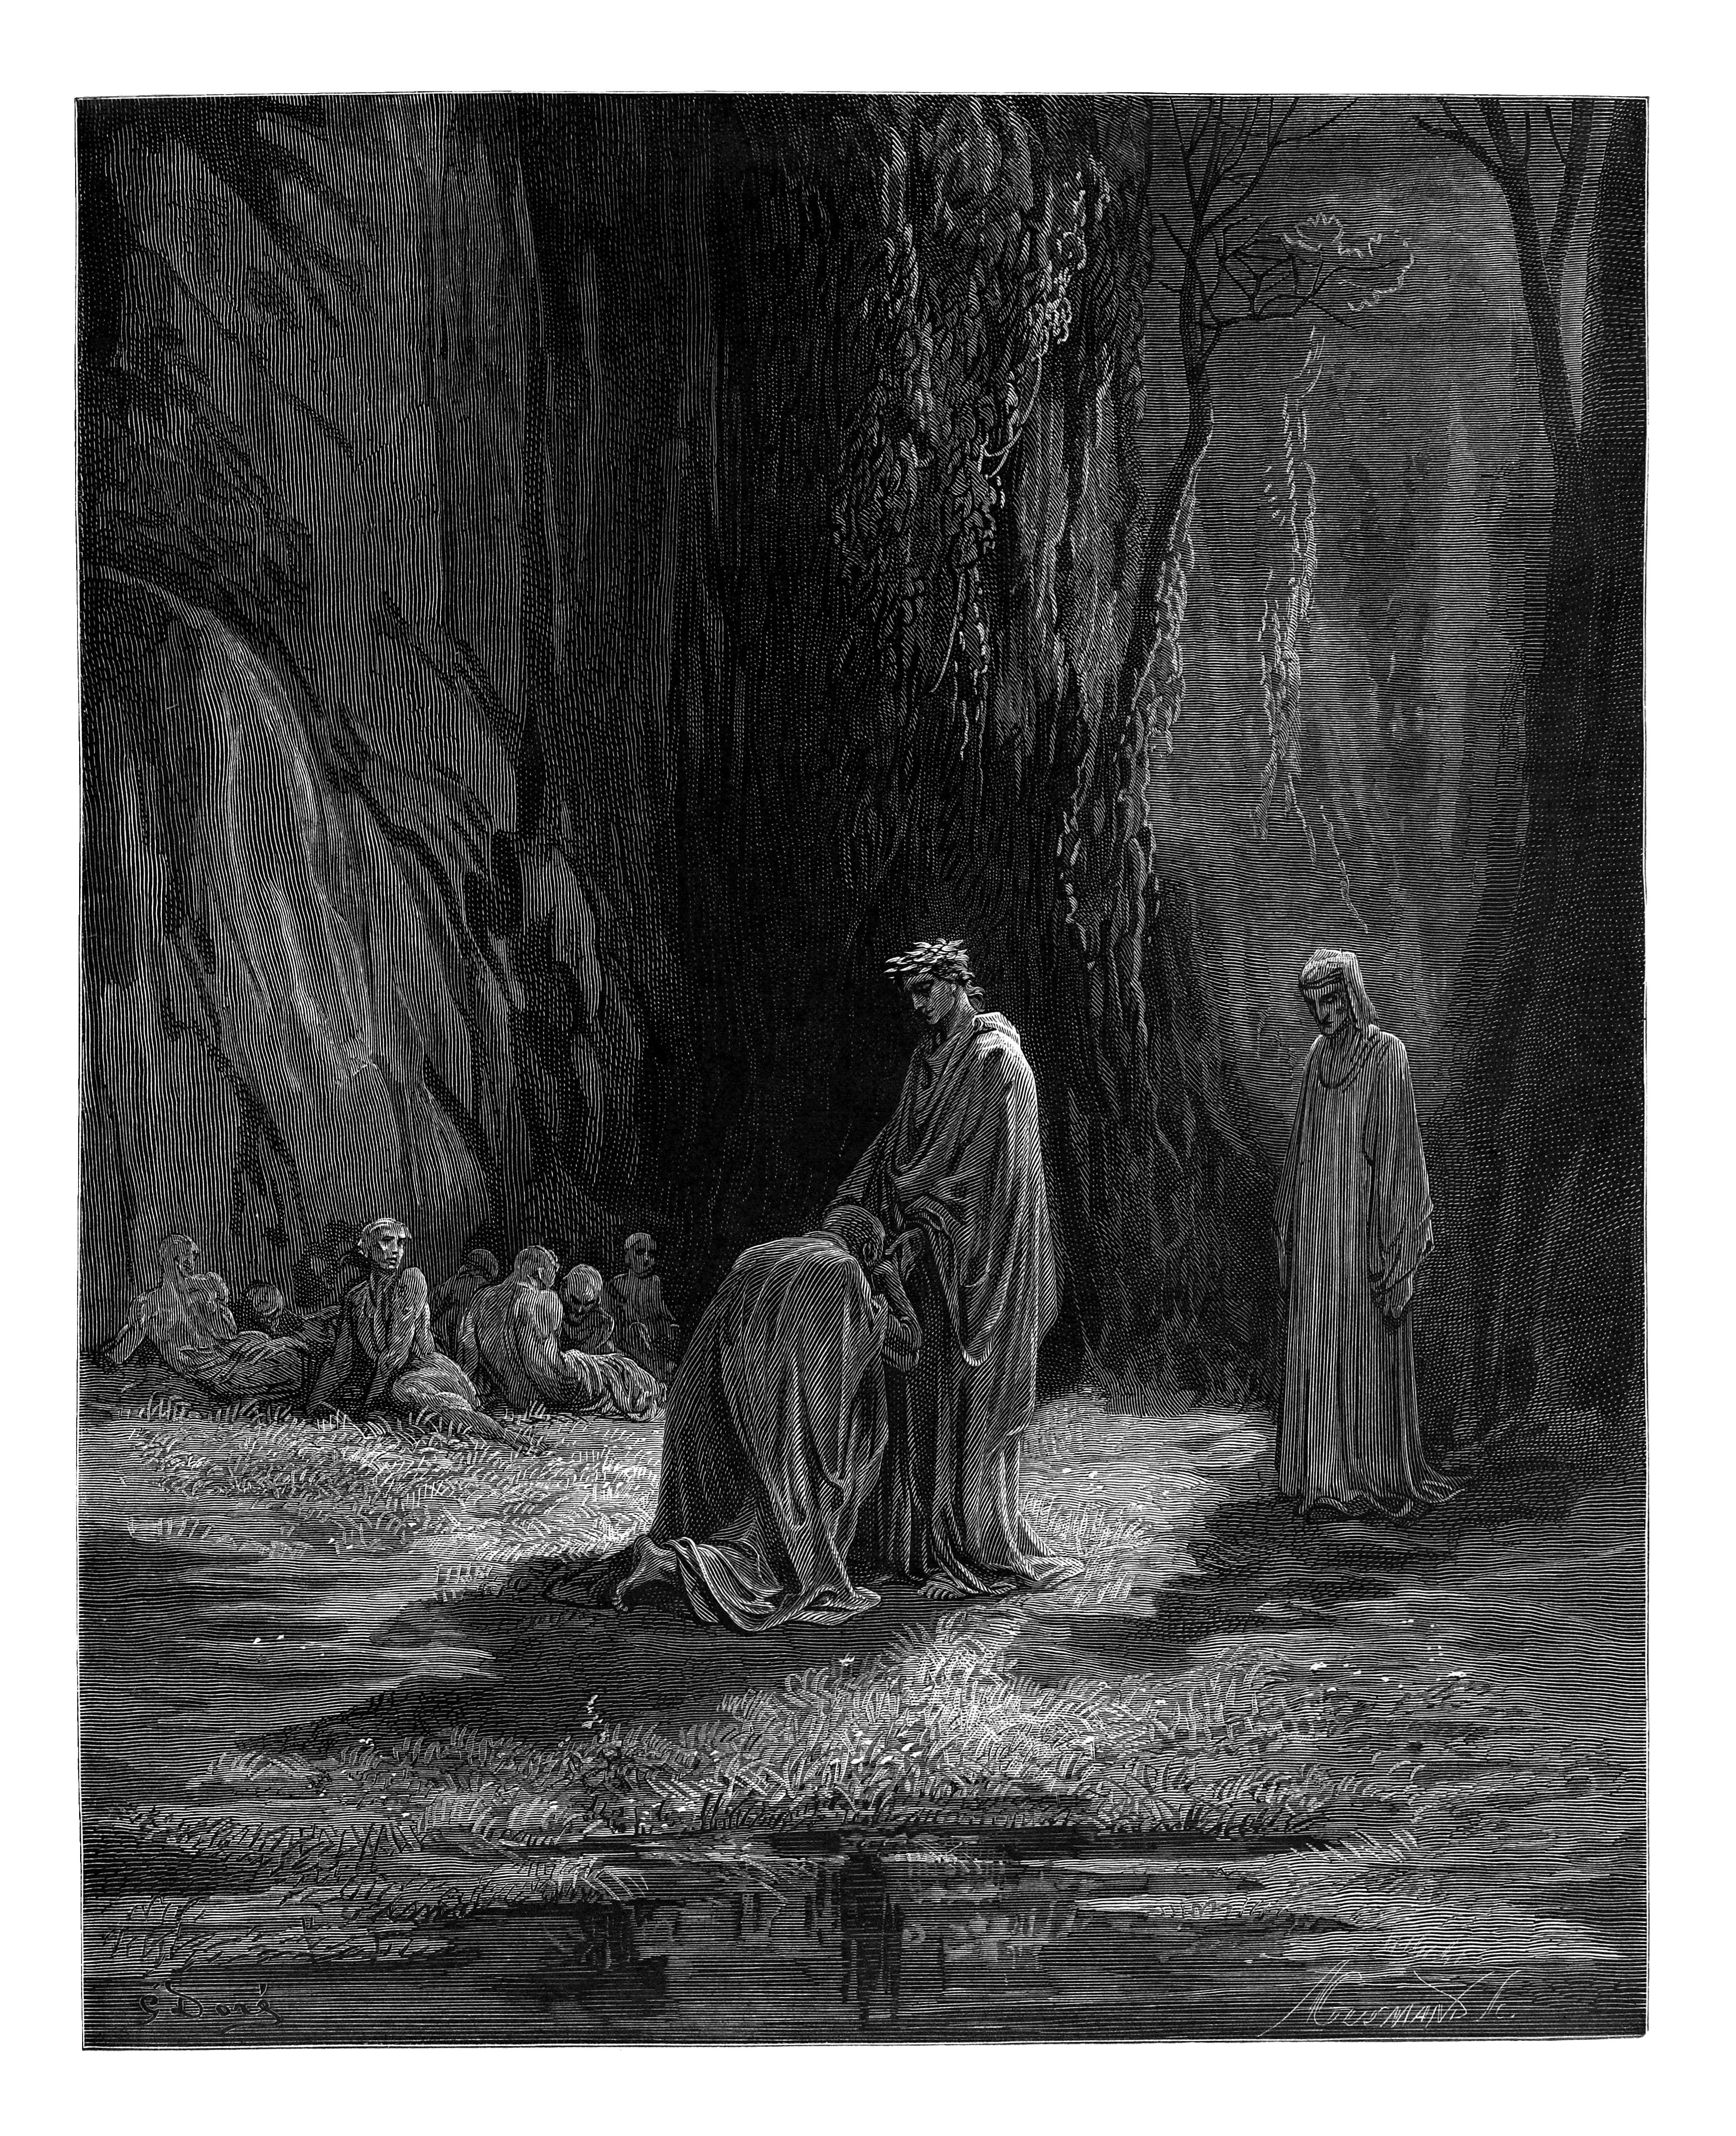
\includegraphics[height=\figsize]{illustrations/book_2/V02, c07(1).jpg}
\end{figure}

\begin{center}
\begin{minipage}{0.8\linewidth}
\textit{\\
"...chin\`o le ciglia,\\e umilmente ritorn\`o ver’ lui,\\e abbracci\`ol là ’ve ’l minor s’appiglia."} \\
—V02, c07(1) \\~\\
\textit{"...downward bent his eyes,\\And drawing near with reverential step,\\Caught him, where of mean estate might clasp\\His lord. …"} \\
—B02, c07(1)
\end{minipage}
\end{center}

\newpage

\section{Canto 07(2)}

\begin{figure}[ht]
\centering
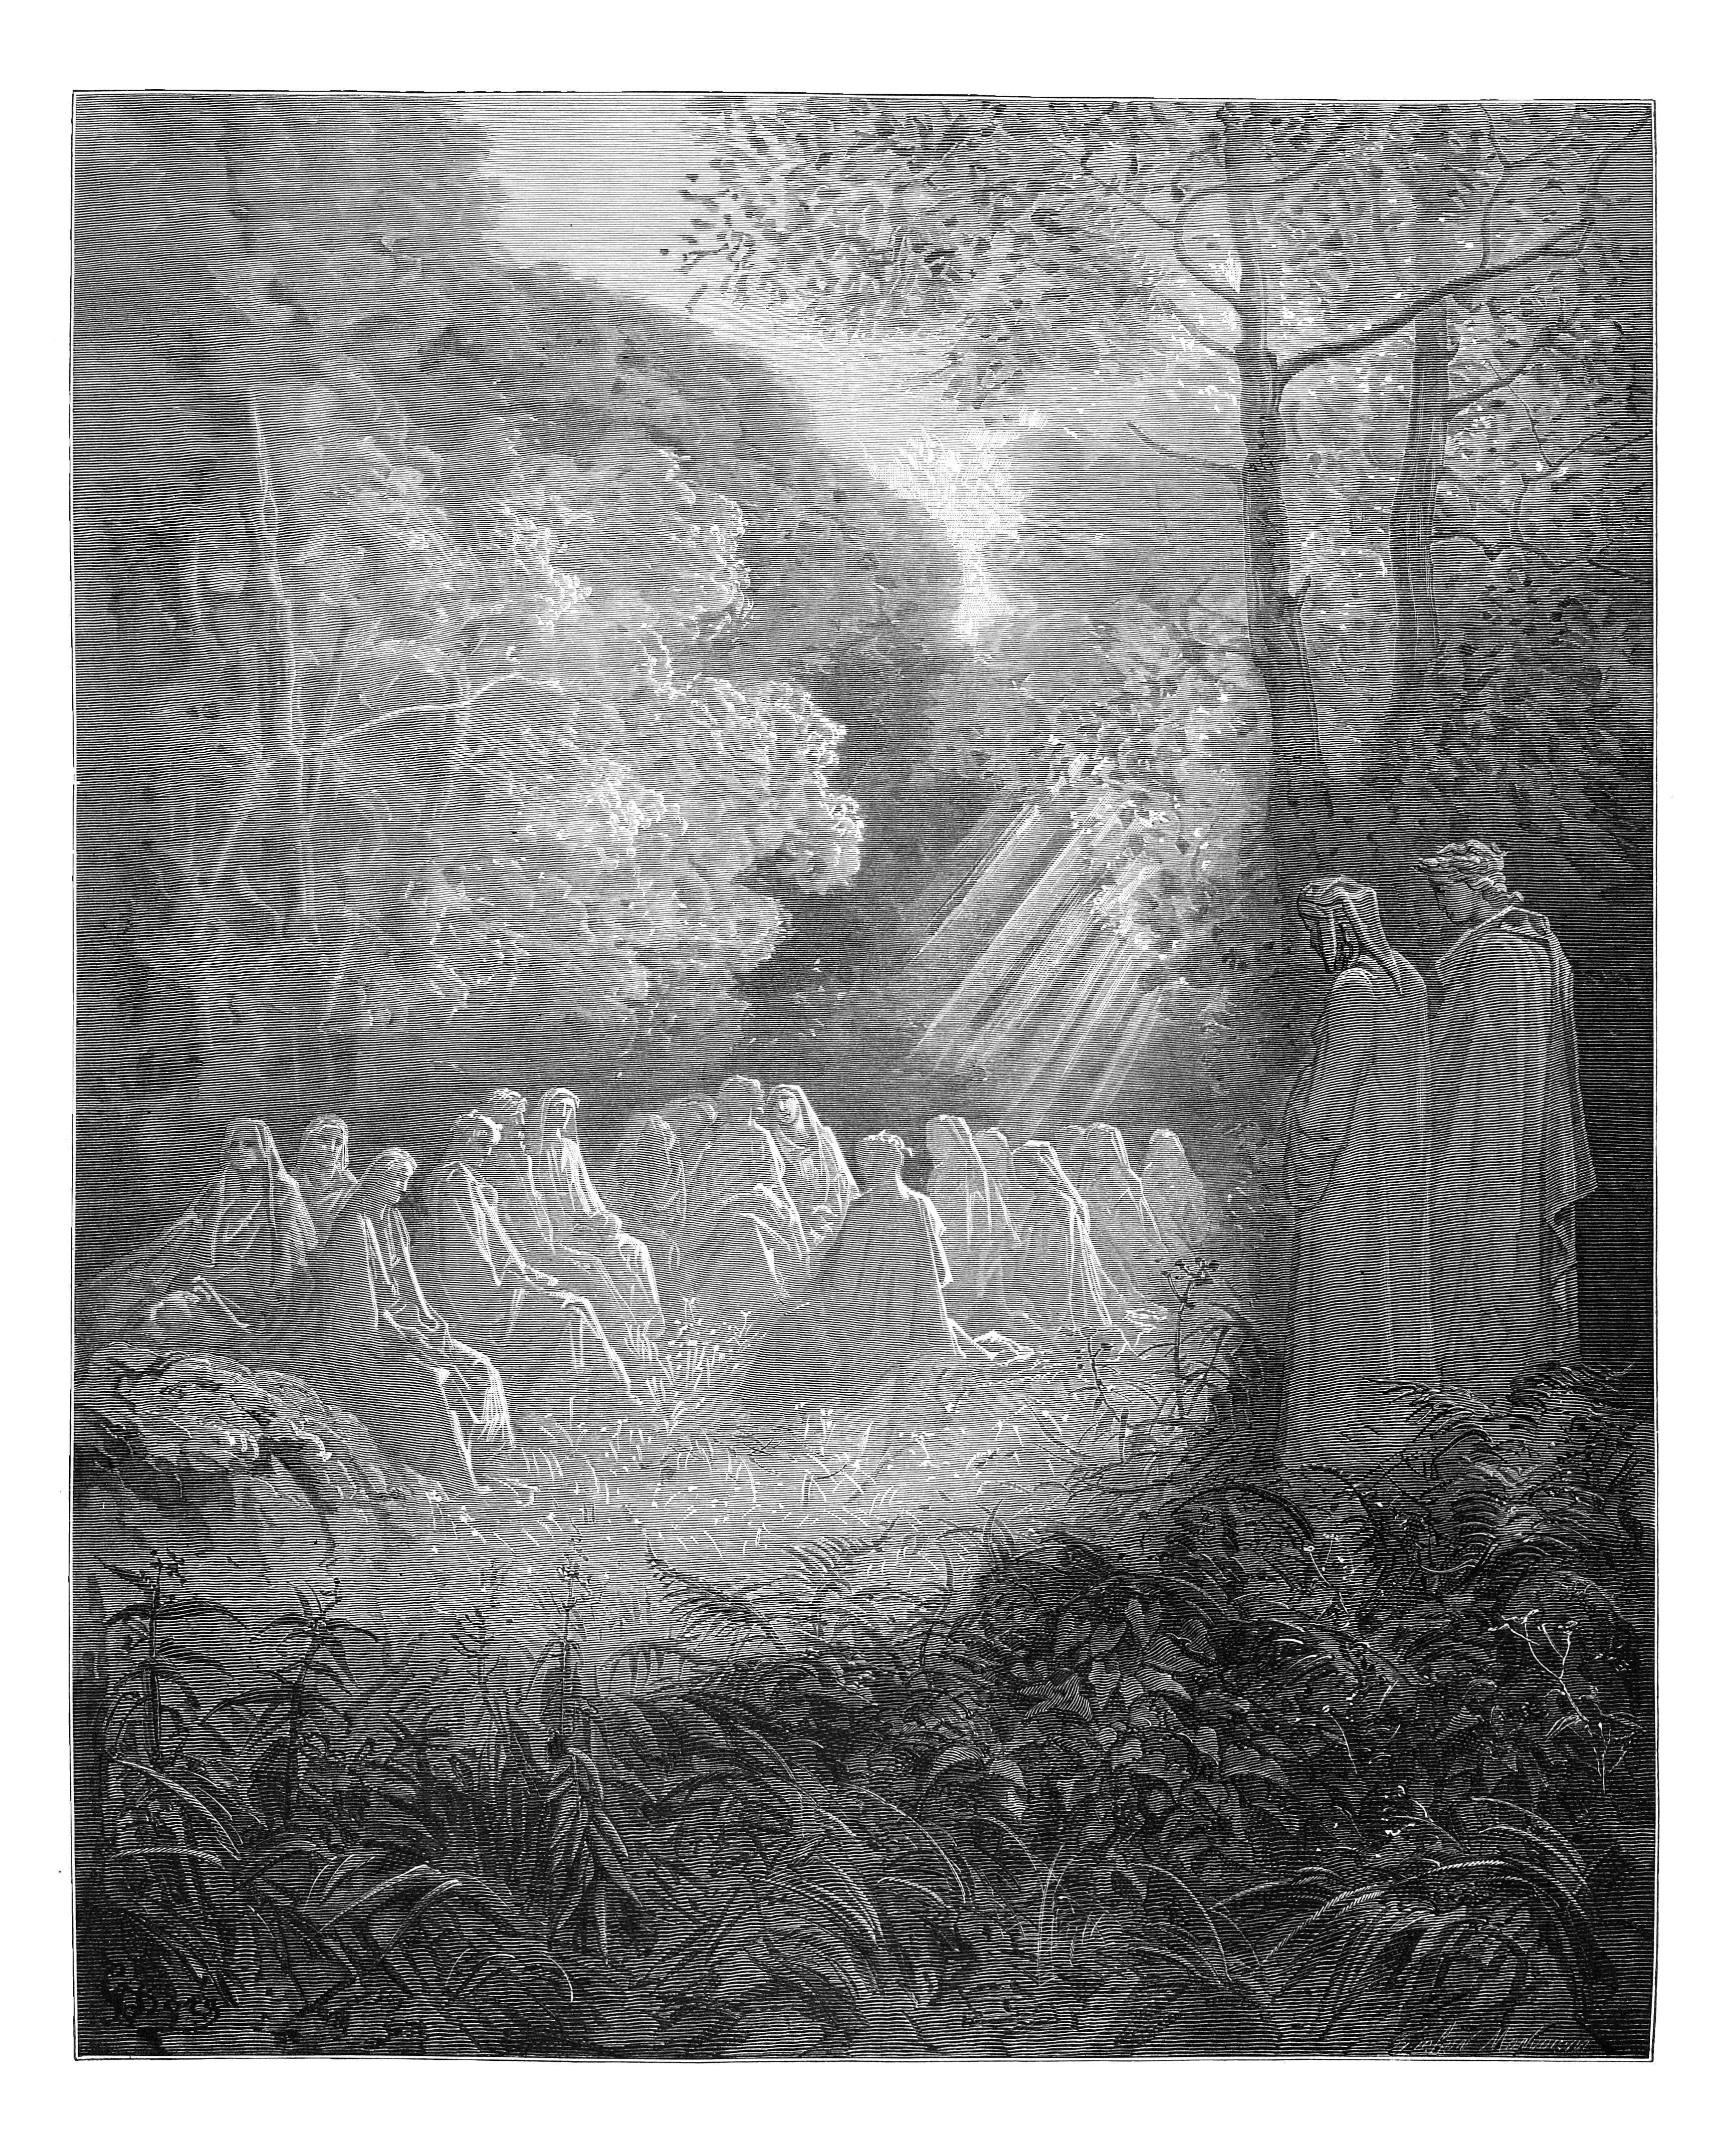
\includegraphics[height=\figsize]{illustrations/book_2/V02, c07(2).jpg}
\end{figure}

\begin{center}
\begin{minipage}{0.8\linewidth}
\textit{\\
"«Salve, Regina» in sul verde e ’n su’ fiori//quindi seder cantando anime vidi,"} \\
—V02, c07(2) \\~\\
\textit{"\textquotesingle Salve Regina,\textquotesingle  on the grass and flowers\\Here chanting I beheld those spirits sit"} \\
—B02, c07(2)
\end{minipage}
\end{center}

\newpage

\section{Canto 08}

\begin{figure}[ht]
\centering
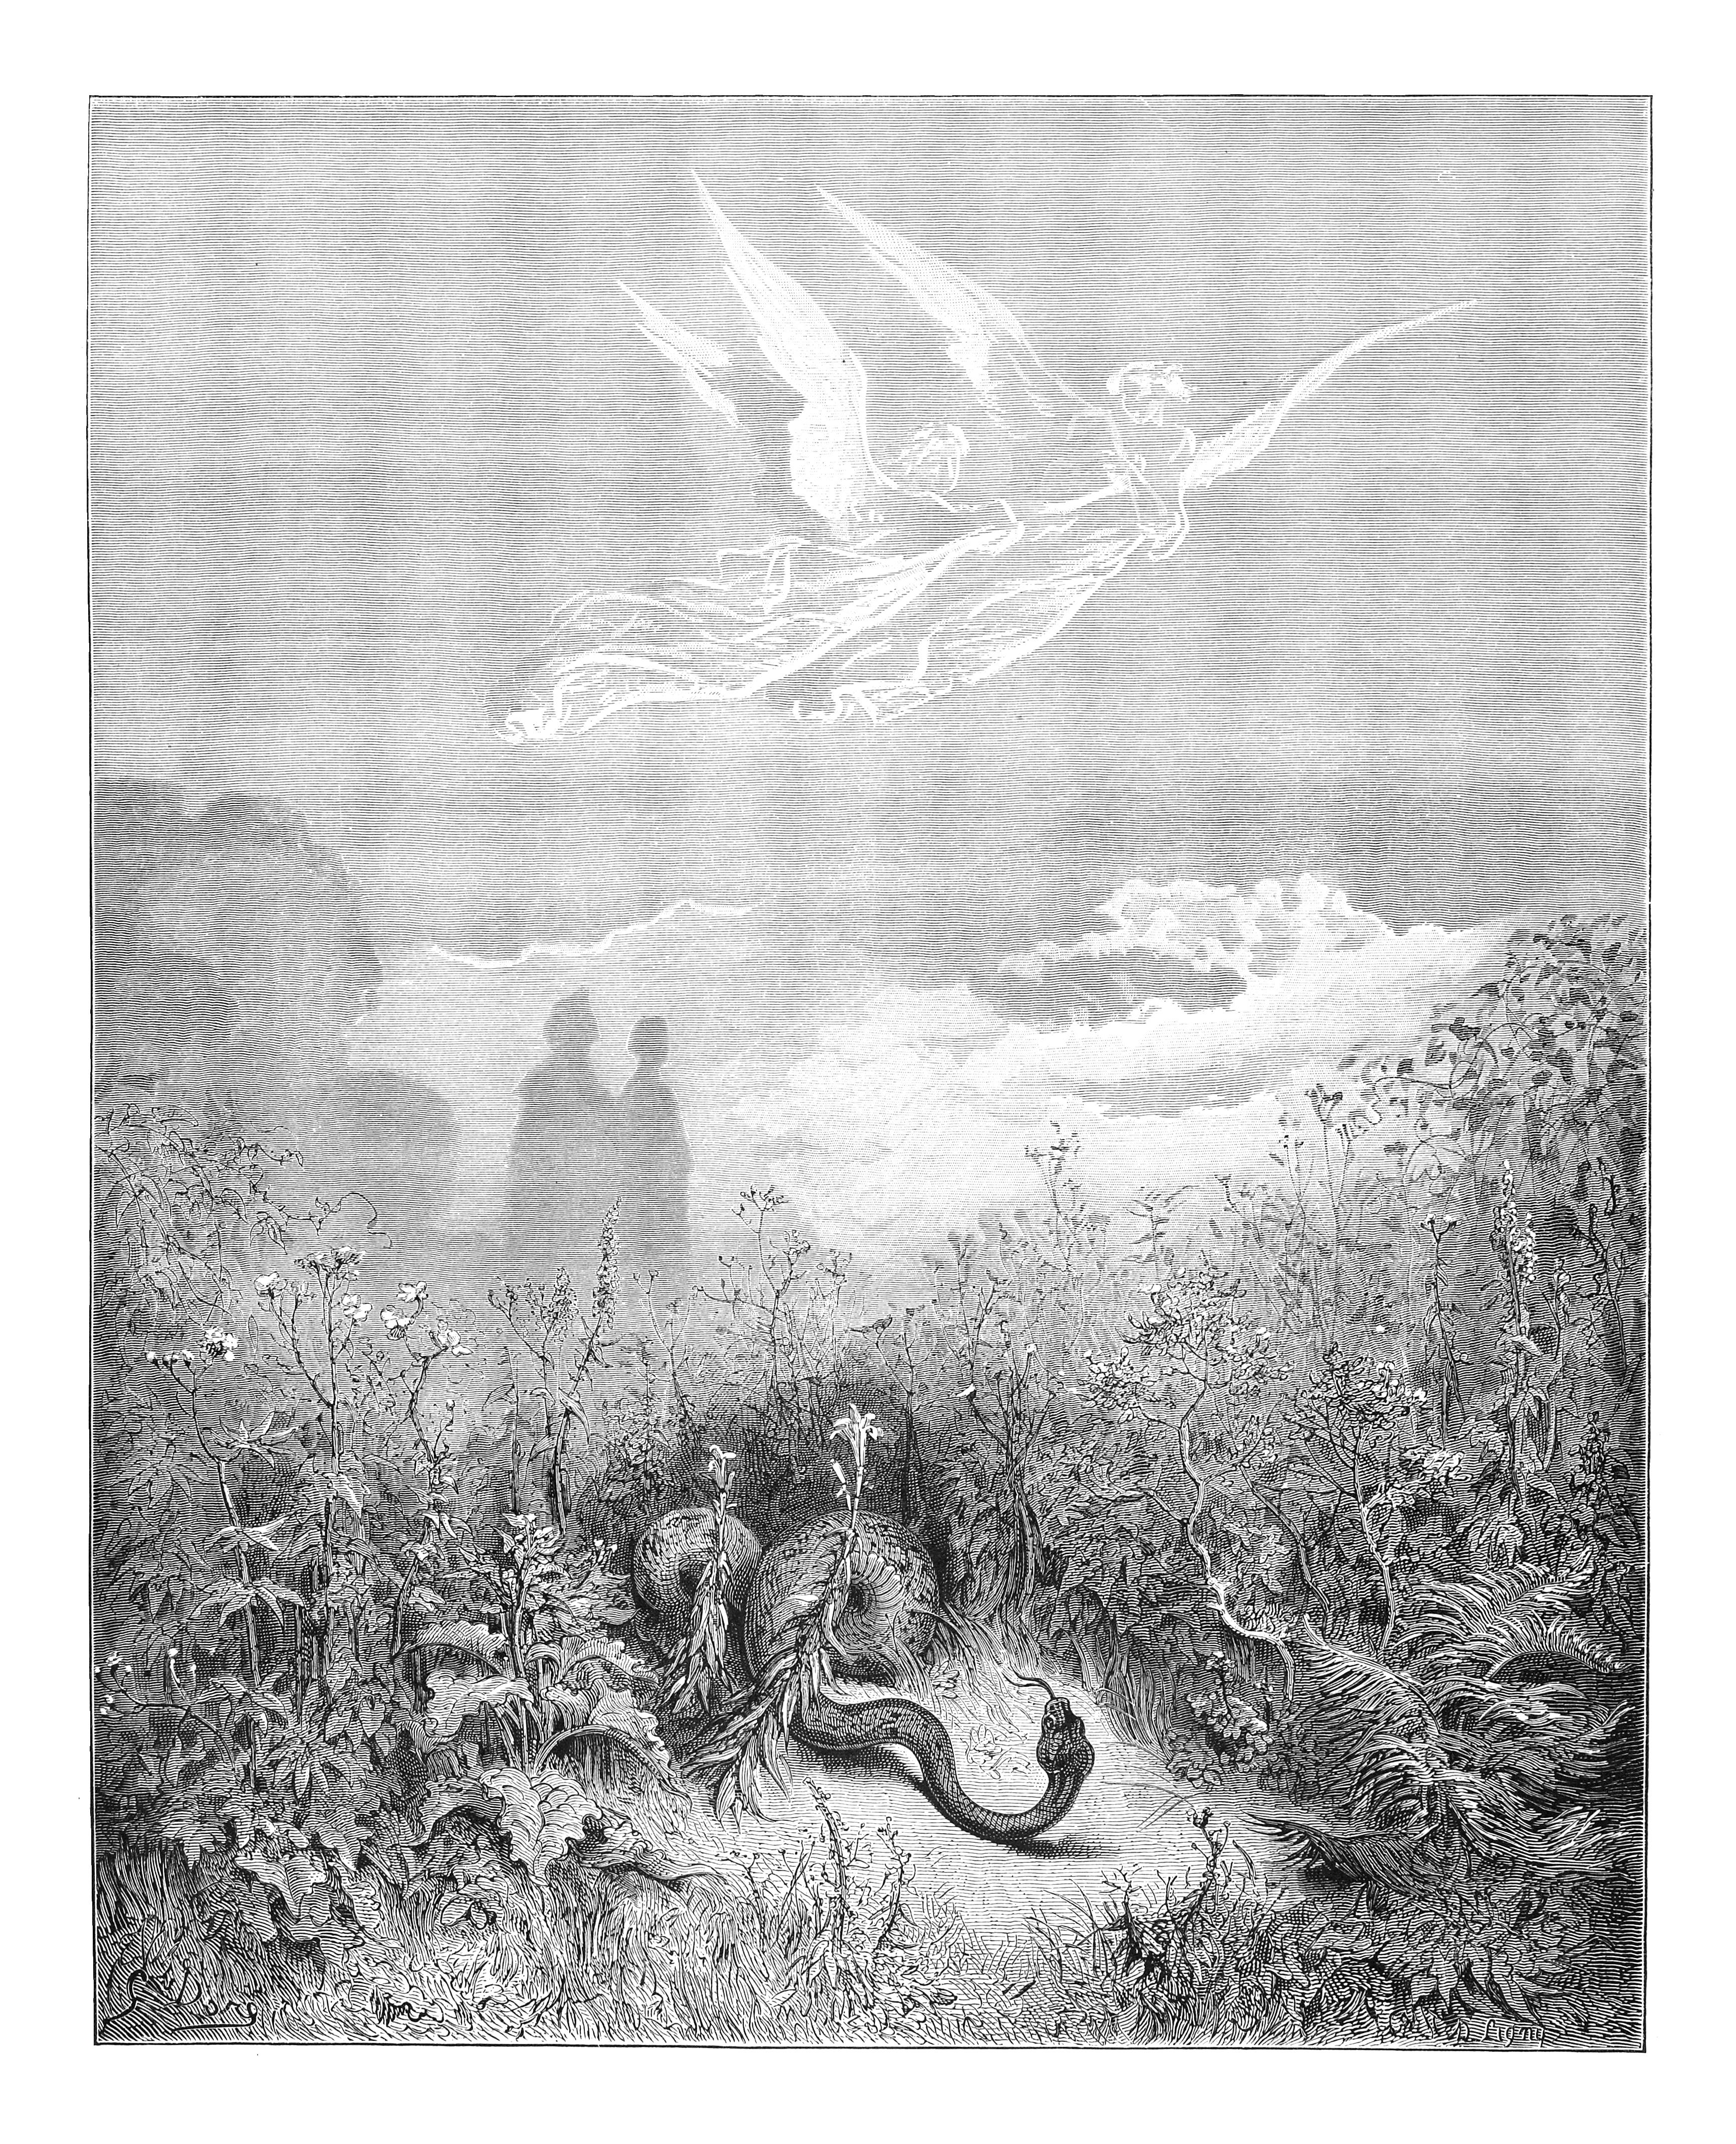
\includegraphics[height=\figsize]{illustrations/book_2/V02, c08.jpg}
\end{figure}

\begin{center}
\begin{minipage}{0.8\linewidth}
\textit{\\
"fugg\`{\i} ’l serpente, e li angeli dier volta,\\suso a le poste rivolando iguali."} \\
—V02, c08 \\~\\
\textit{"The serpent fled; and to their stations back\\The angels up retum'd with equal flight."} \\
—B02, c08
\end{minipage}
\end{center}

\newpage

\section{Canto 09(1)}

\begin{figure}[ht]
\centering
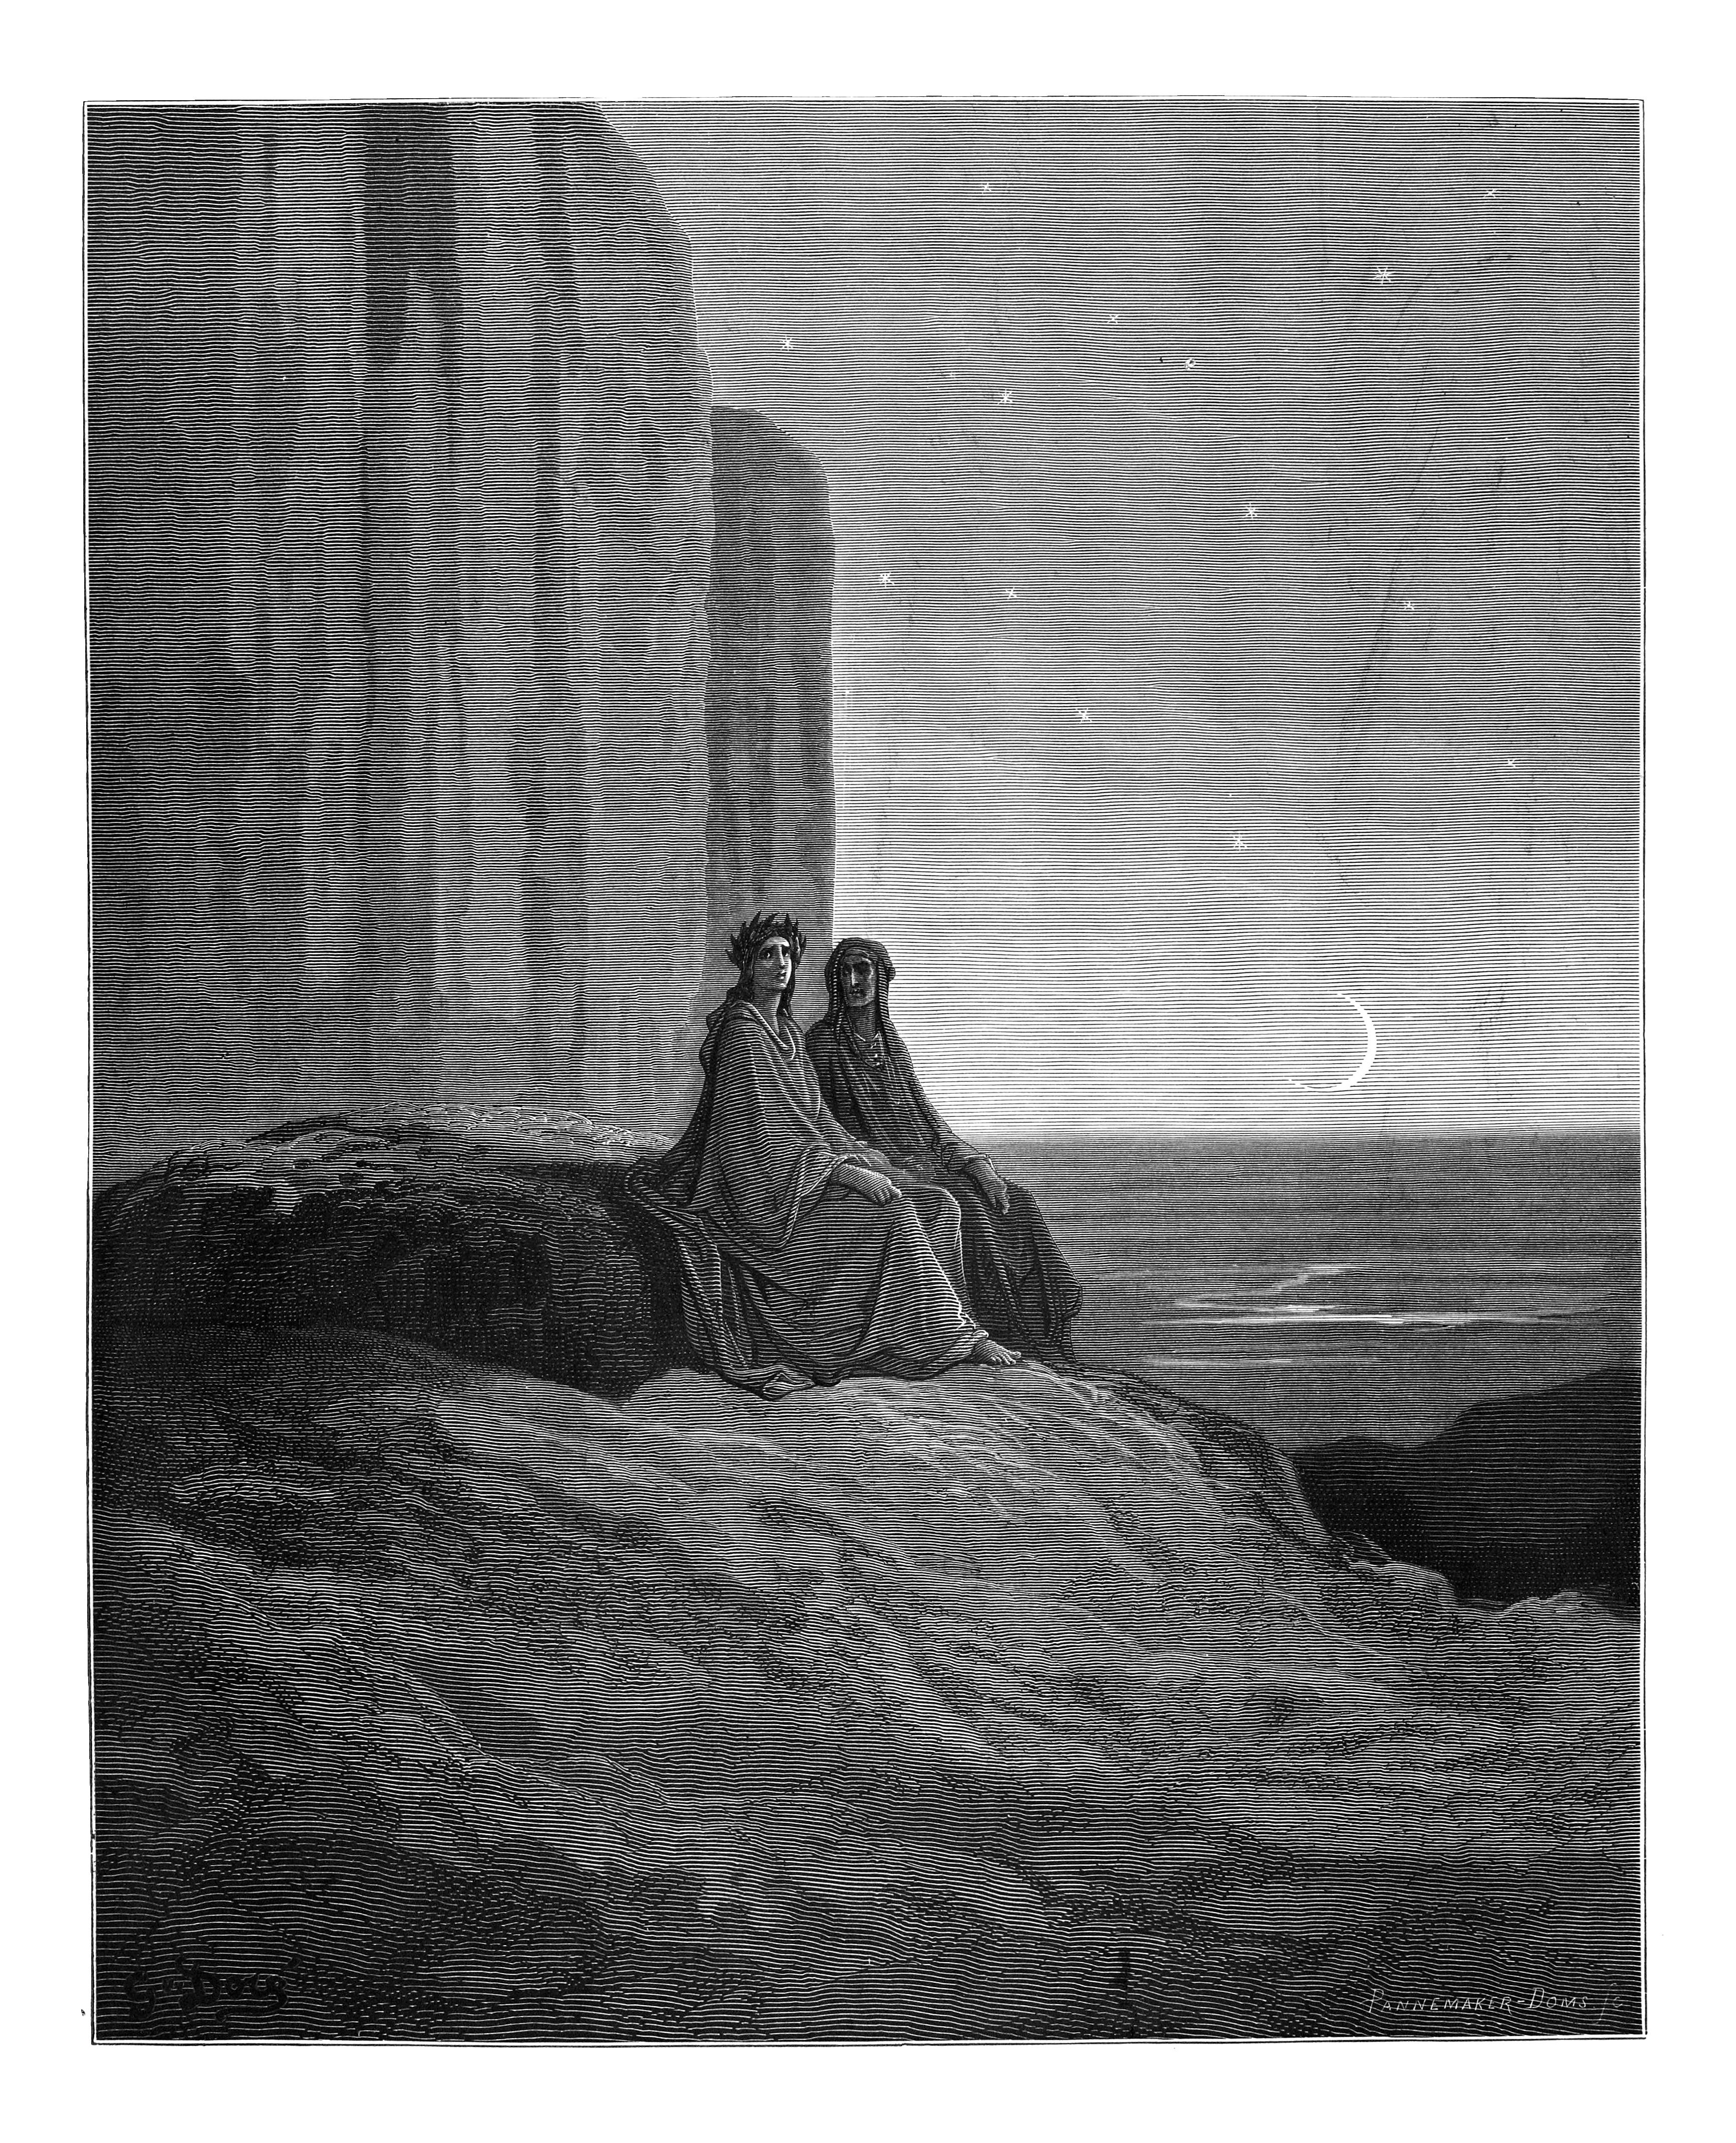
\includegraphics[height=\figsize]{illustrations/book_2/V02, c09(1).jpg}
\end{figure}

\begin{center}
\begin{minipage}{0.8\linewidth}
\textit{\\
"La concubina di Titone antico\\già s’imbiancava al balco d’oriente,\\fuor de le braccia del suo dolce amico;"} \\
—V02, c09(1) \\~\\
\textit{"Now the fair consort of Tithonus old,\\Arisen from her mate's beloved arms,\\Look'd palely o'er the eastern cliff: …"} \\
—B02, c09(1)
\end{minipage}
\end{center}

\newpage

\section{Canto 09(2)}

\begin{figure}[ht]
\centering
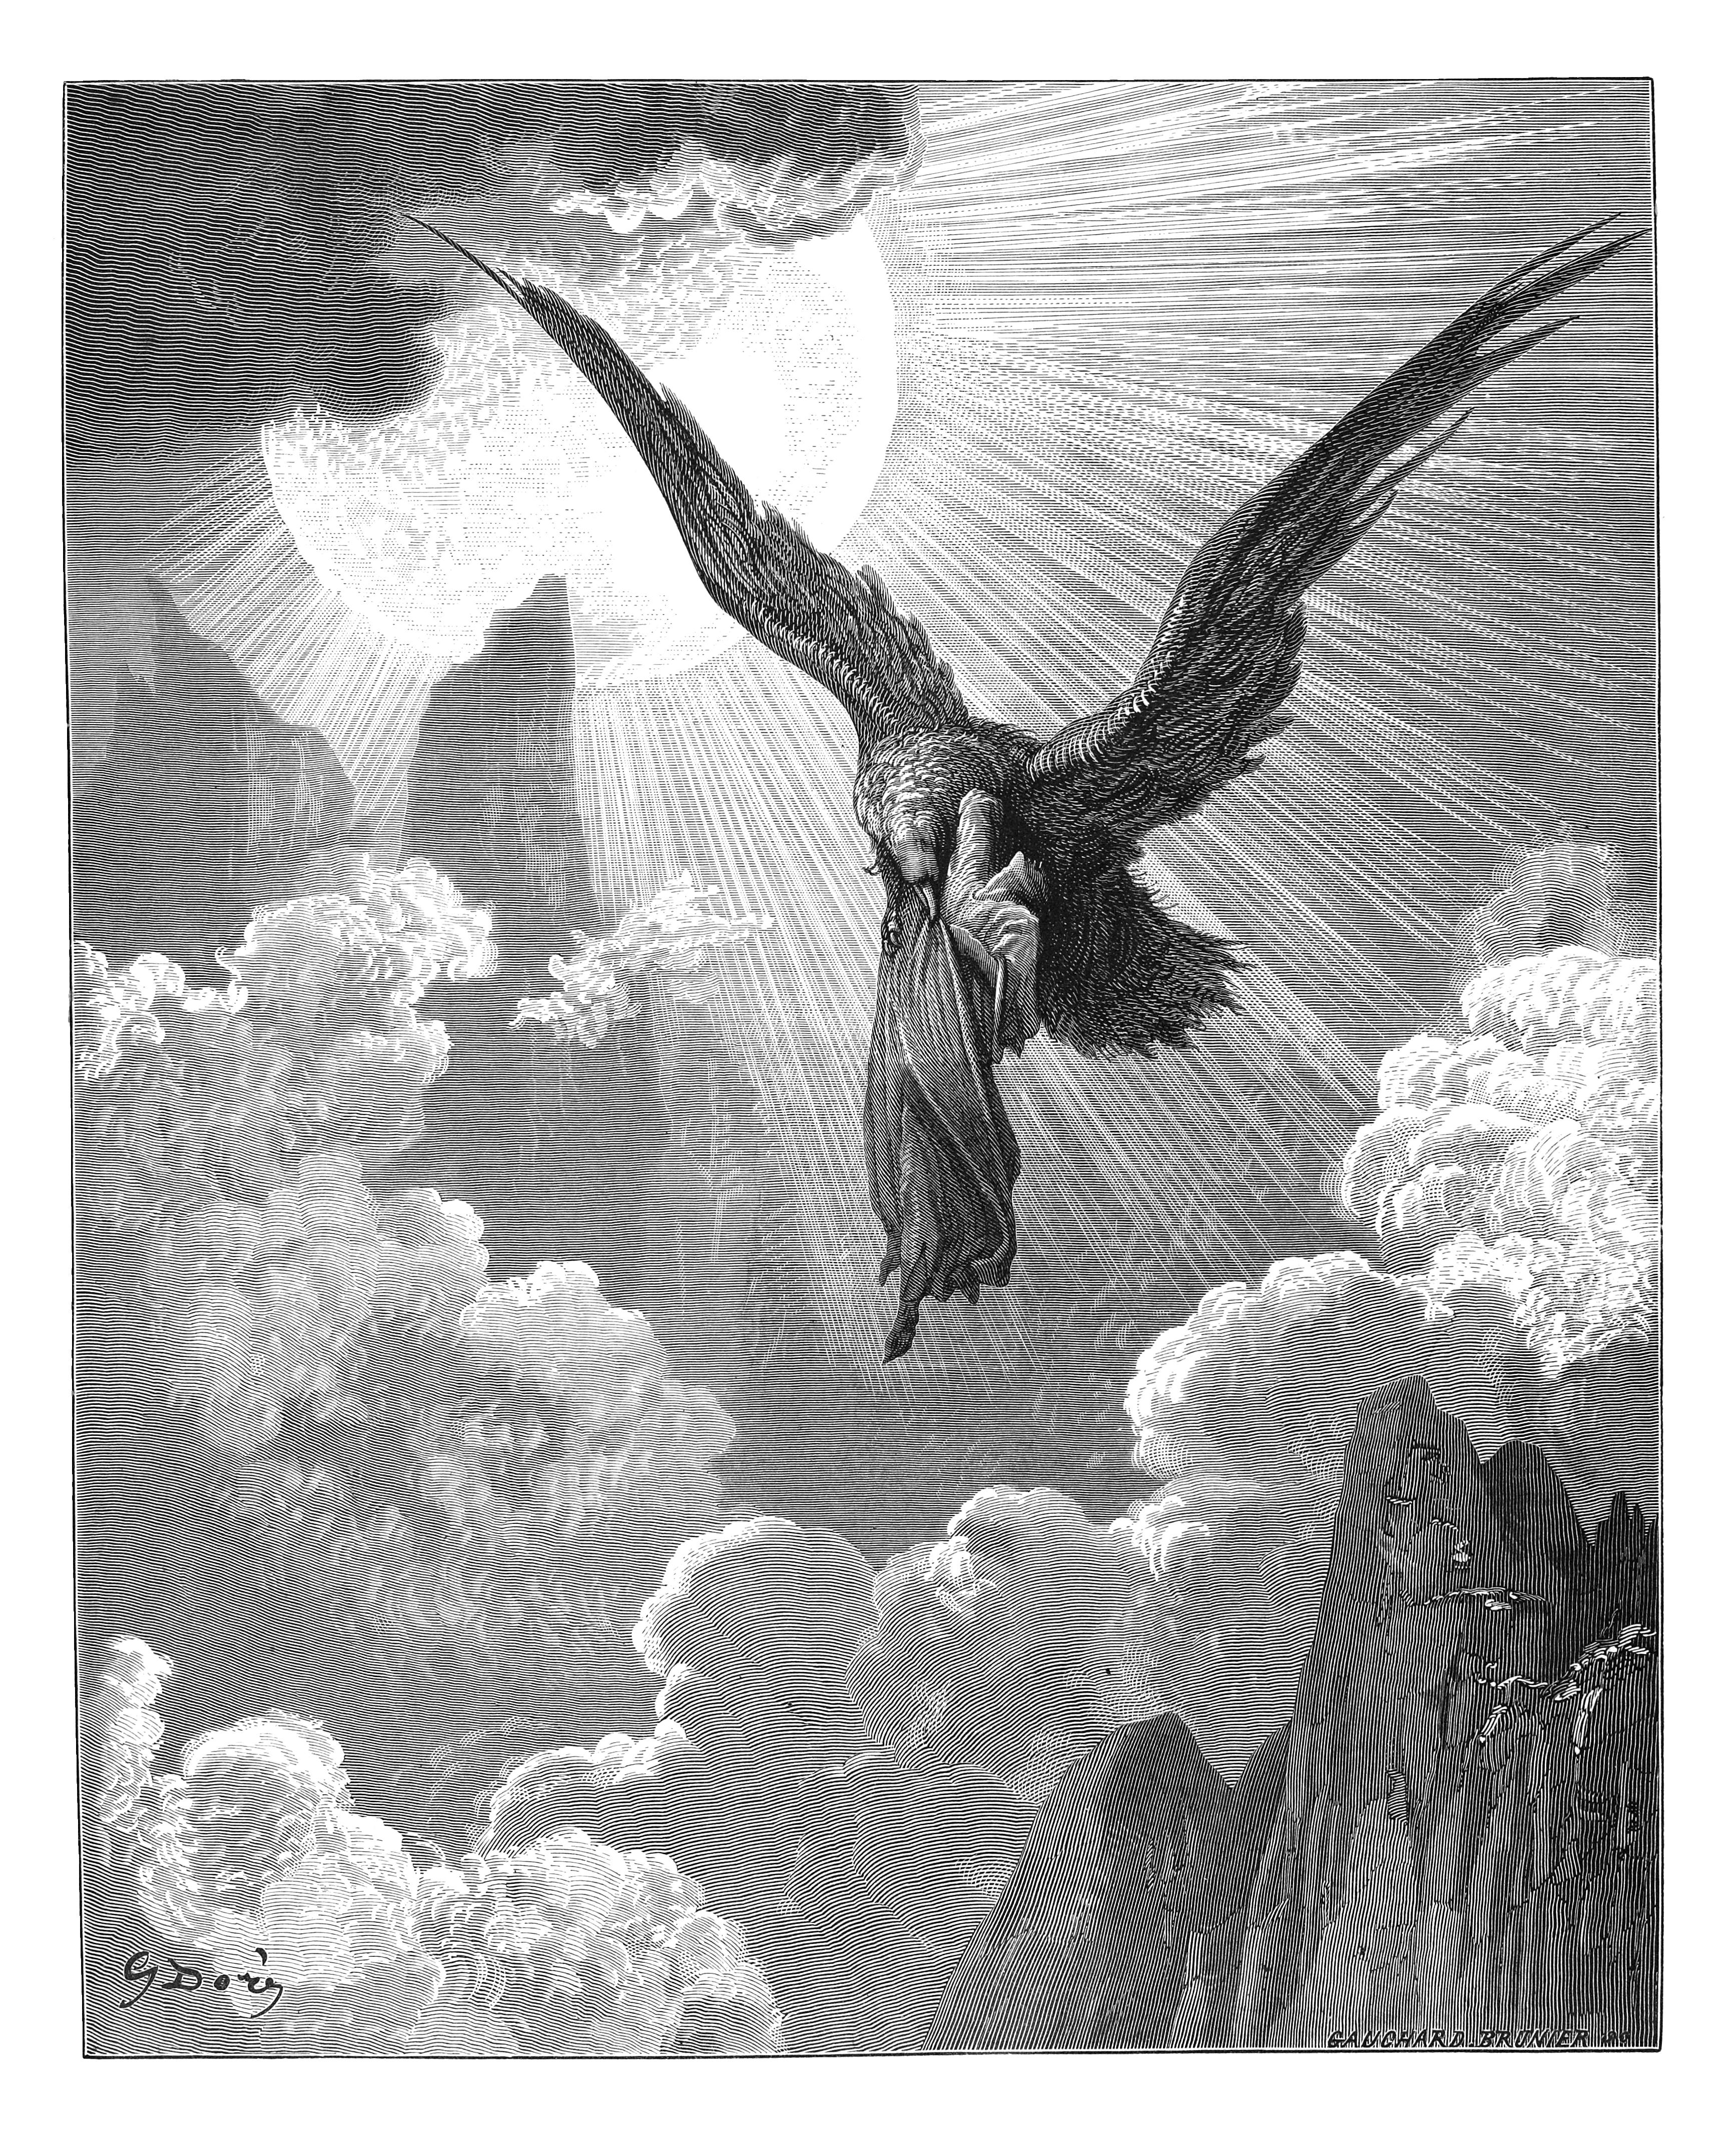
\includegraphics[height=\figsize]{illustrations/book_2/V02, c09(2).jpg}
\end{figure}

\begin{center}
\begin{minipage}{0.8\linewidth}
\textit{\\
"terribil come folgor discendesse,\\e me rapisse suso infino al foco."} \\
—V02, c09(2) \\~\\
\textit{"Terrible as the lightning rush'd he down,\\And snatch'd me upward even to the fire."} \\
—B02, c09(2)
\end{minipage}
\end{center}

\newpage

\section{Canto 09(3)}

\begin{figure}[ht]
\centering
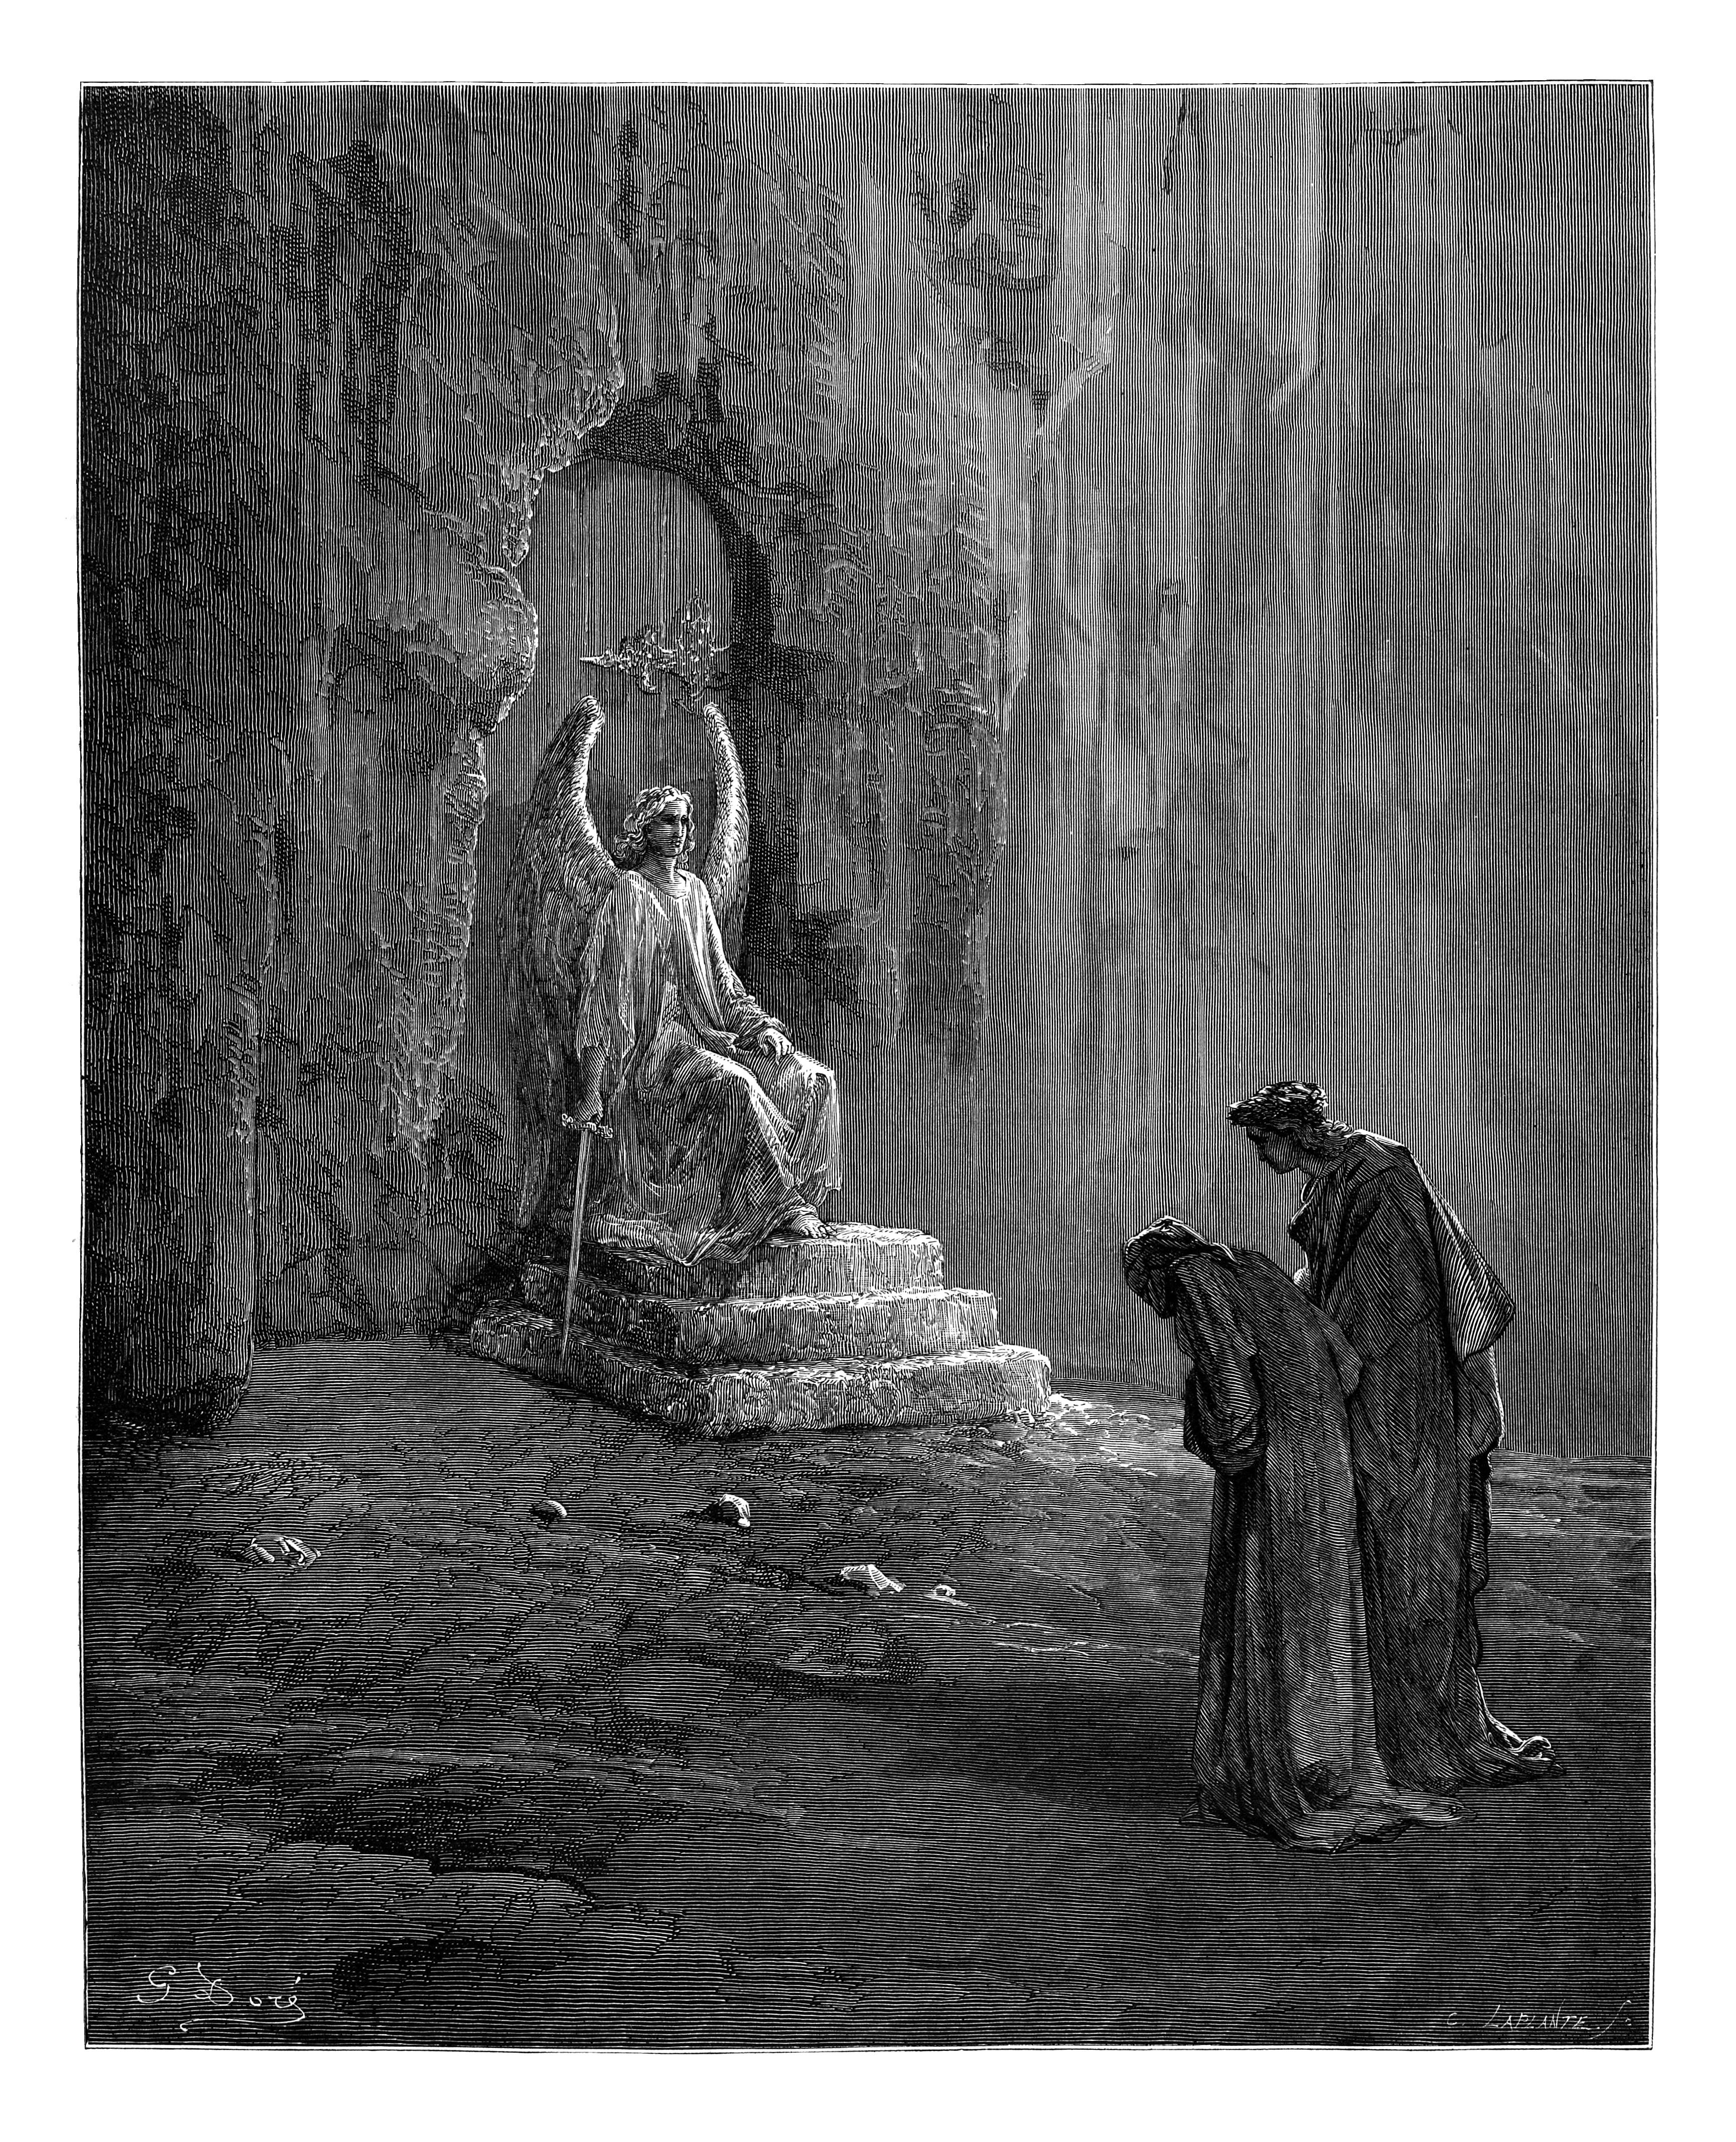
\includegraphics[height=\figsize]{illustrations/book_2/V02, c09(3).jpg}
\end{figure}

\begin{center}
\begin{minipage}{0.8\linewidth}
\textit{\\
"vidil seder sovra ’l grado sovrano,\\tal ne la faccia ch’io non lo soffersi;"} \\
—V02, c09(3) \\~\\
\textit{"I mark'd him seated on the highest step,\\In visage such, as past my power to bear."} \\
—B02, c09(3)
\end{minipage}
\end{center}

\newpage

\section{Canto 10}

\begin{figure}[ht]
\centering
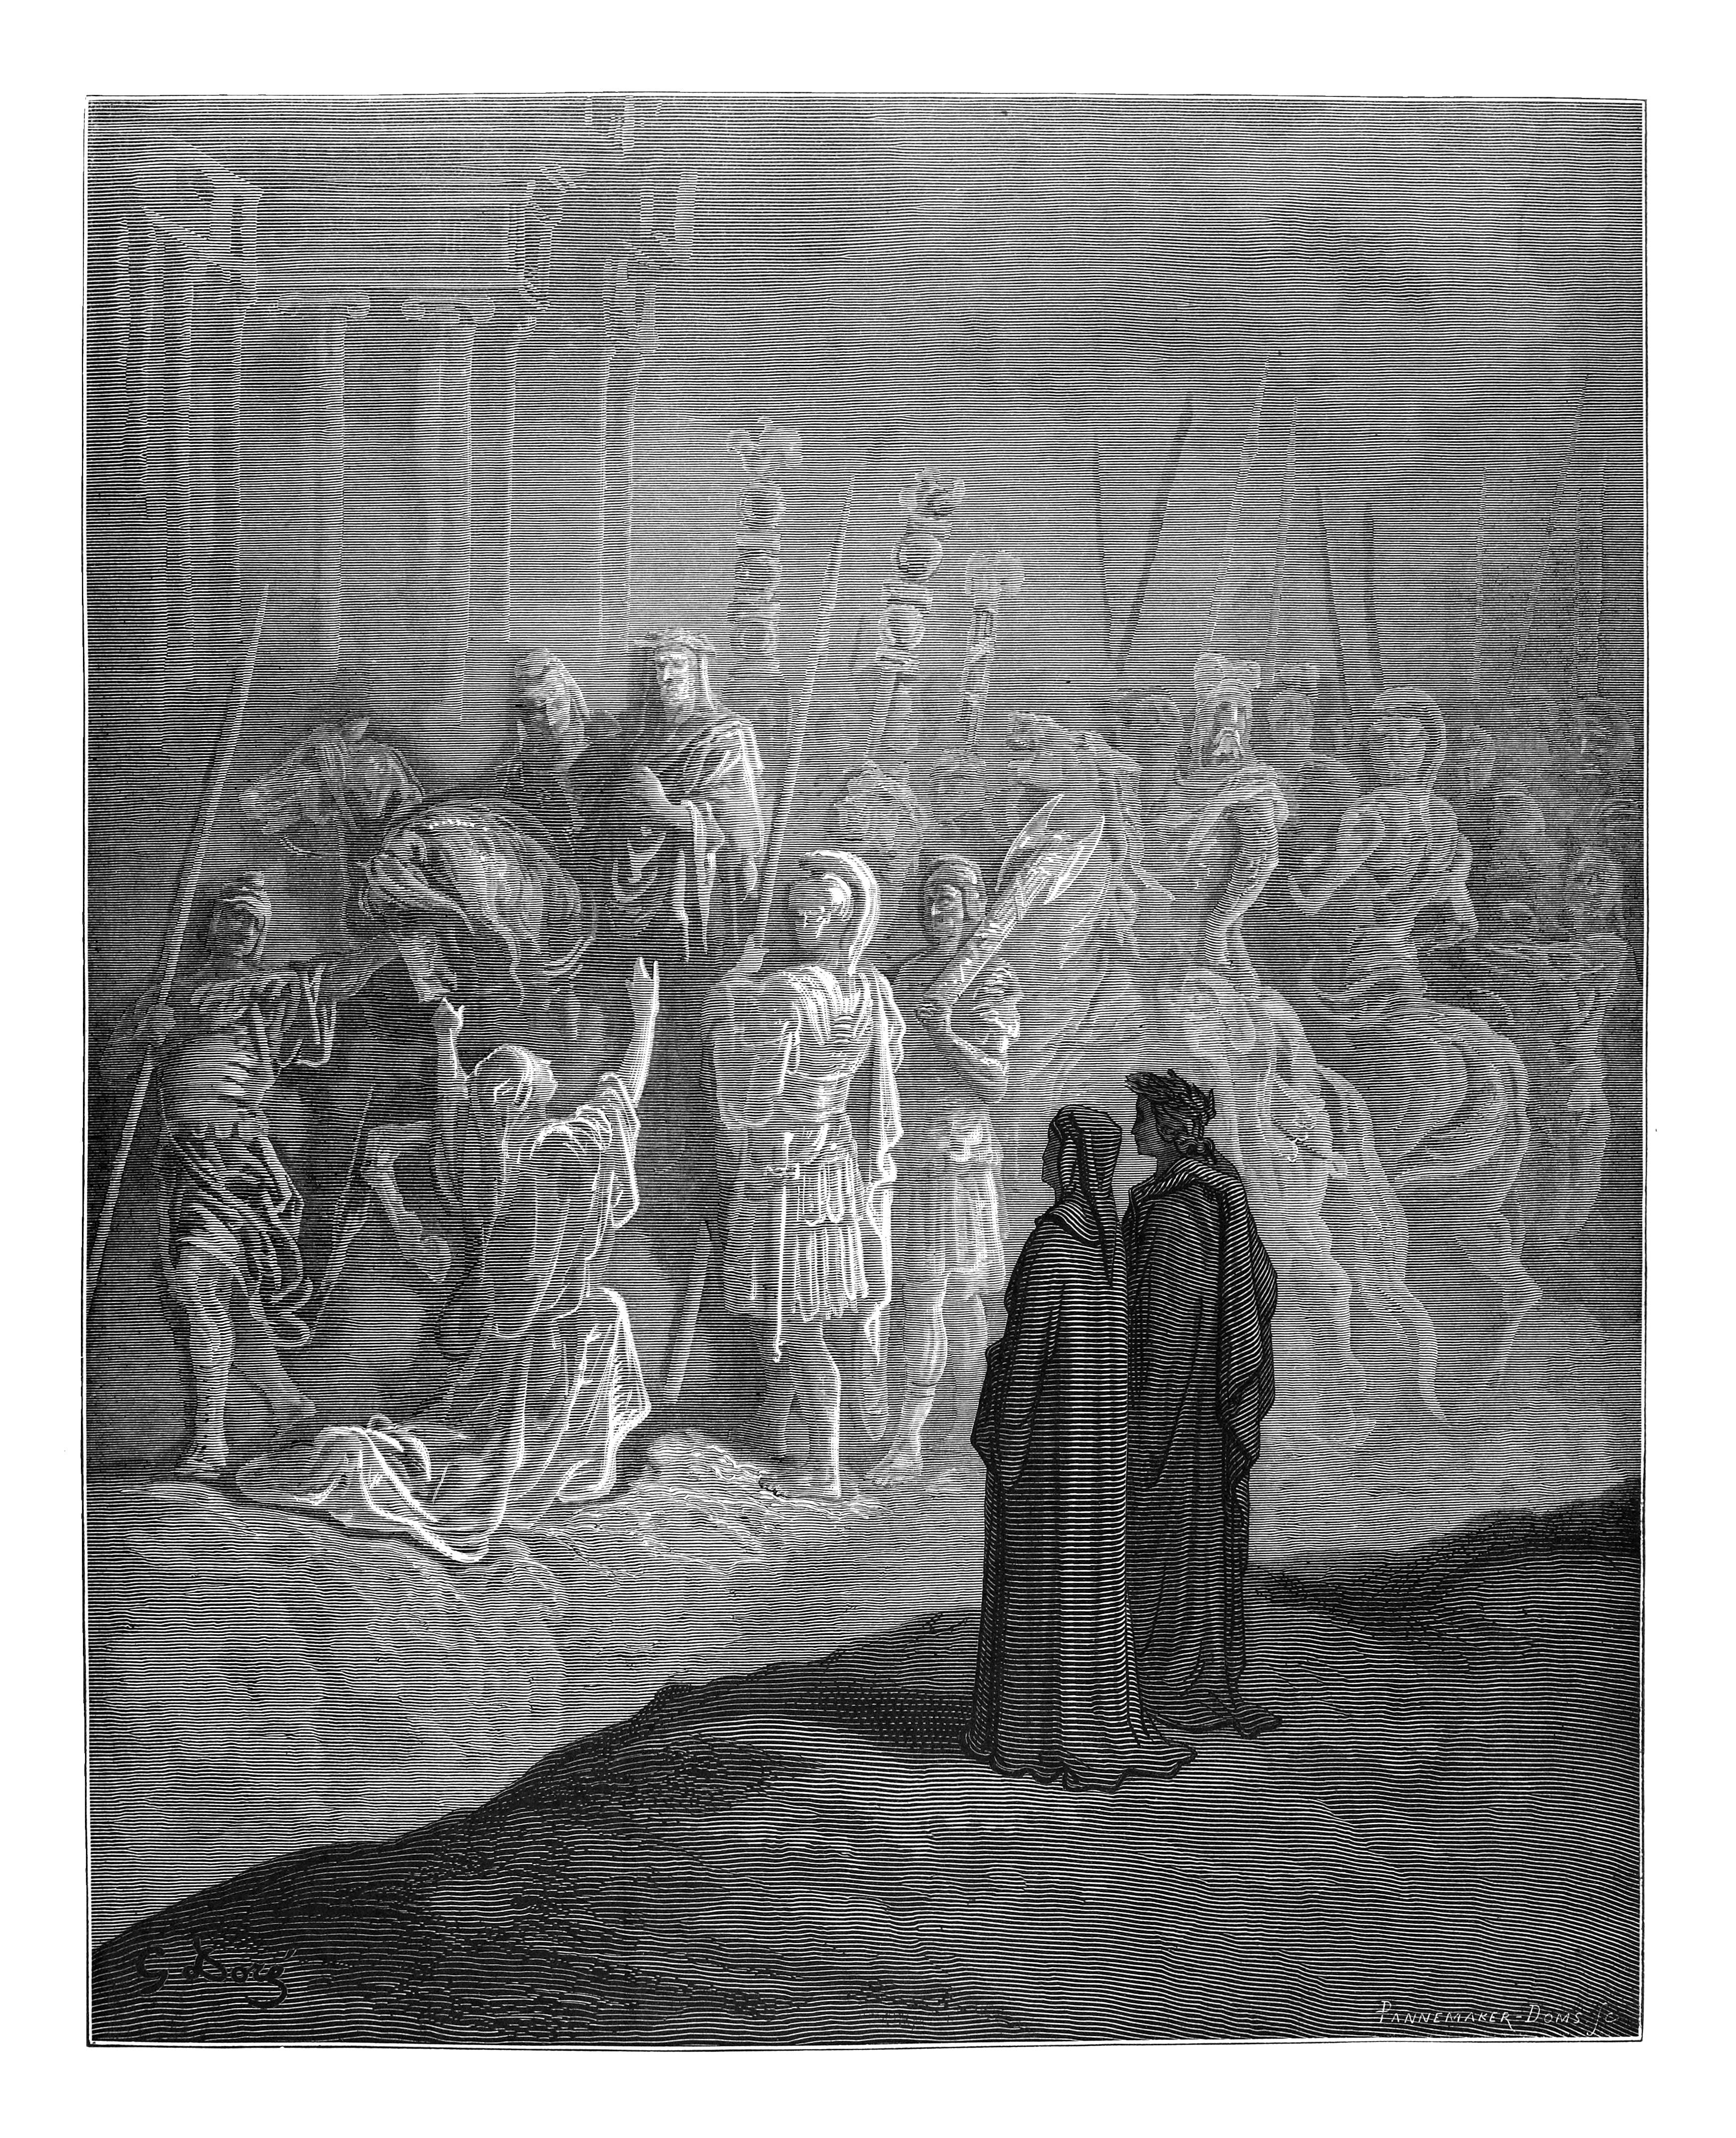
\includegraphics[height=\figsize]{illustrations/book_2/V02, c10.jpg}
\end{figure}

\begin{center}
\begin{minipage}{0.8\linewidth}
\textit{\\
"...non pur Policleto,\\ma la natura lì avrebbe scorno."} \\
—V02, c10 \\~\\
\textit{"...not there alone\\Had Polycletus, but e'en nature's self\\Been sham'd. …"} \\
—B02, c10
\end{minipage}
\end{center}

\newpage

\section{Canto 11}

\begin{figure}[ht]
\centering
\includegraphics[height=\figsize]{illustrations/book_2/V02, c11.jpg}
\end{figure}

\begin{center}
\begin{minipage}{0.8\linewidth}
\textit{\\
"quell’ombre orando, andavan sotto ’l pondo,\\simile a quel che tal volta si sogna,"} \\
—V02, c11 \\~\\
\textit{"Those spirits went beneath a weight like that\\We sometimes feel in dreams, …"} \\
—B02, c11
\end{minipage}
\end{center}

\newpage

\section{Canto 12}

\begin{figure}[ht]
\centering
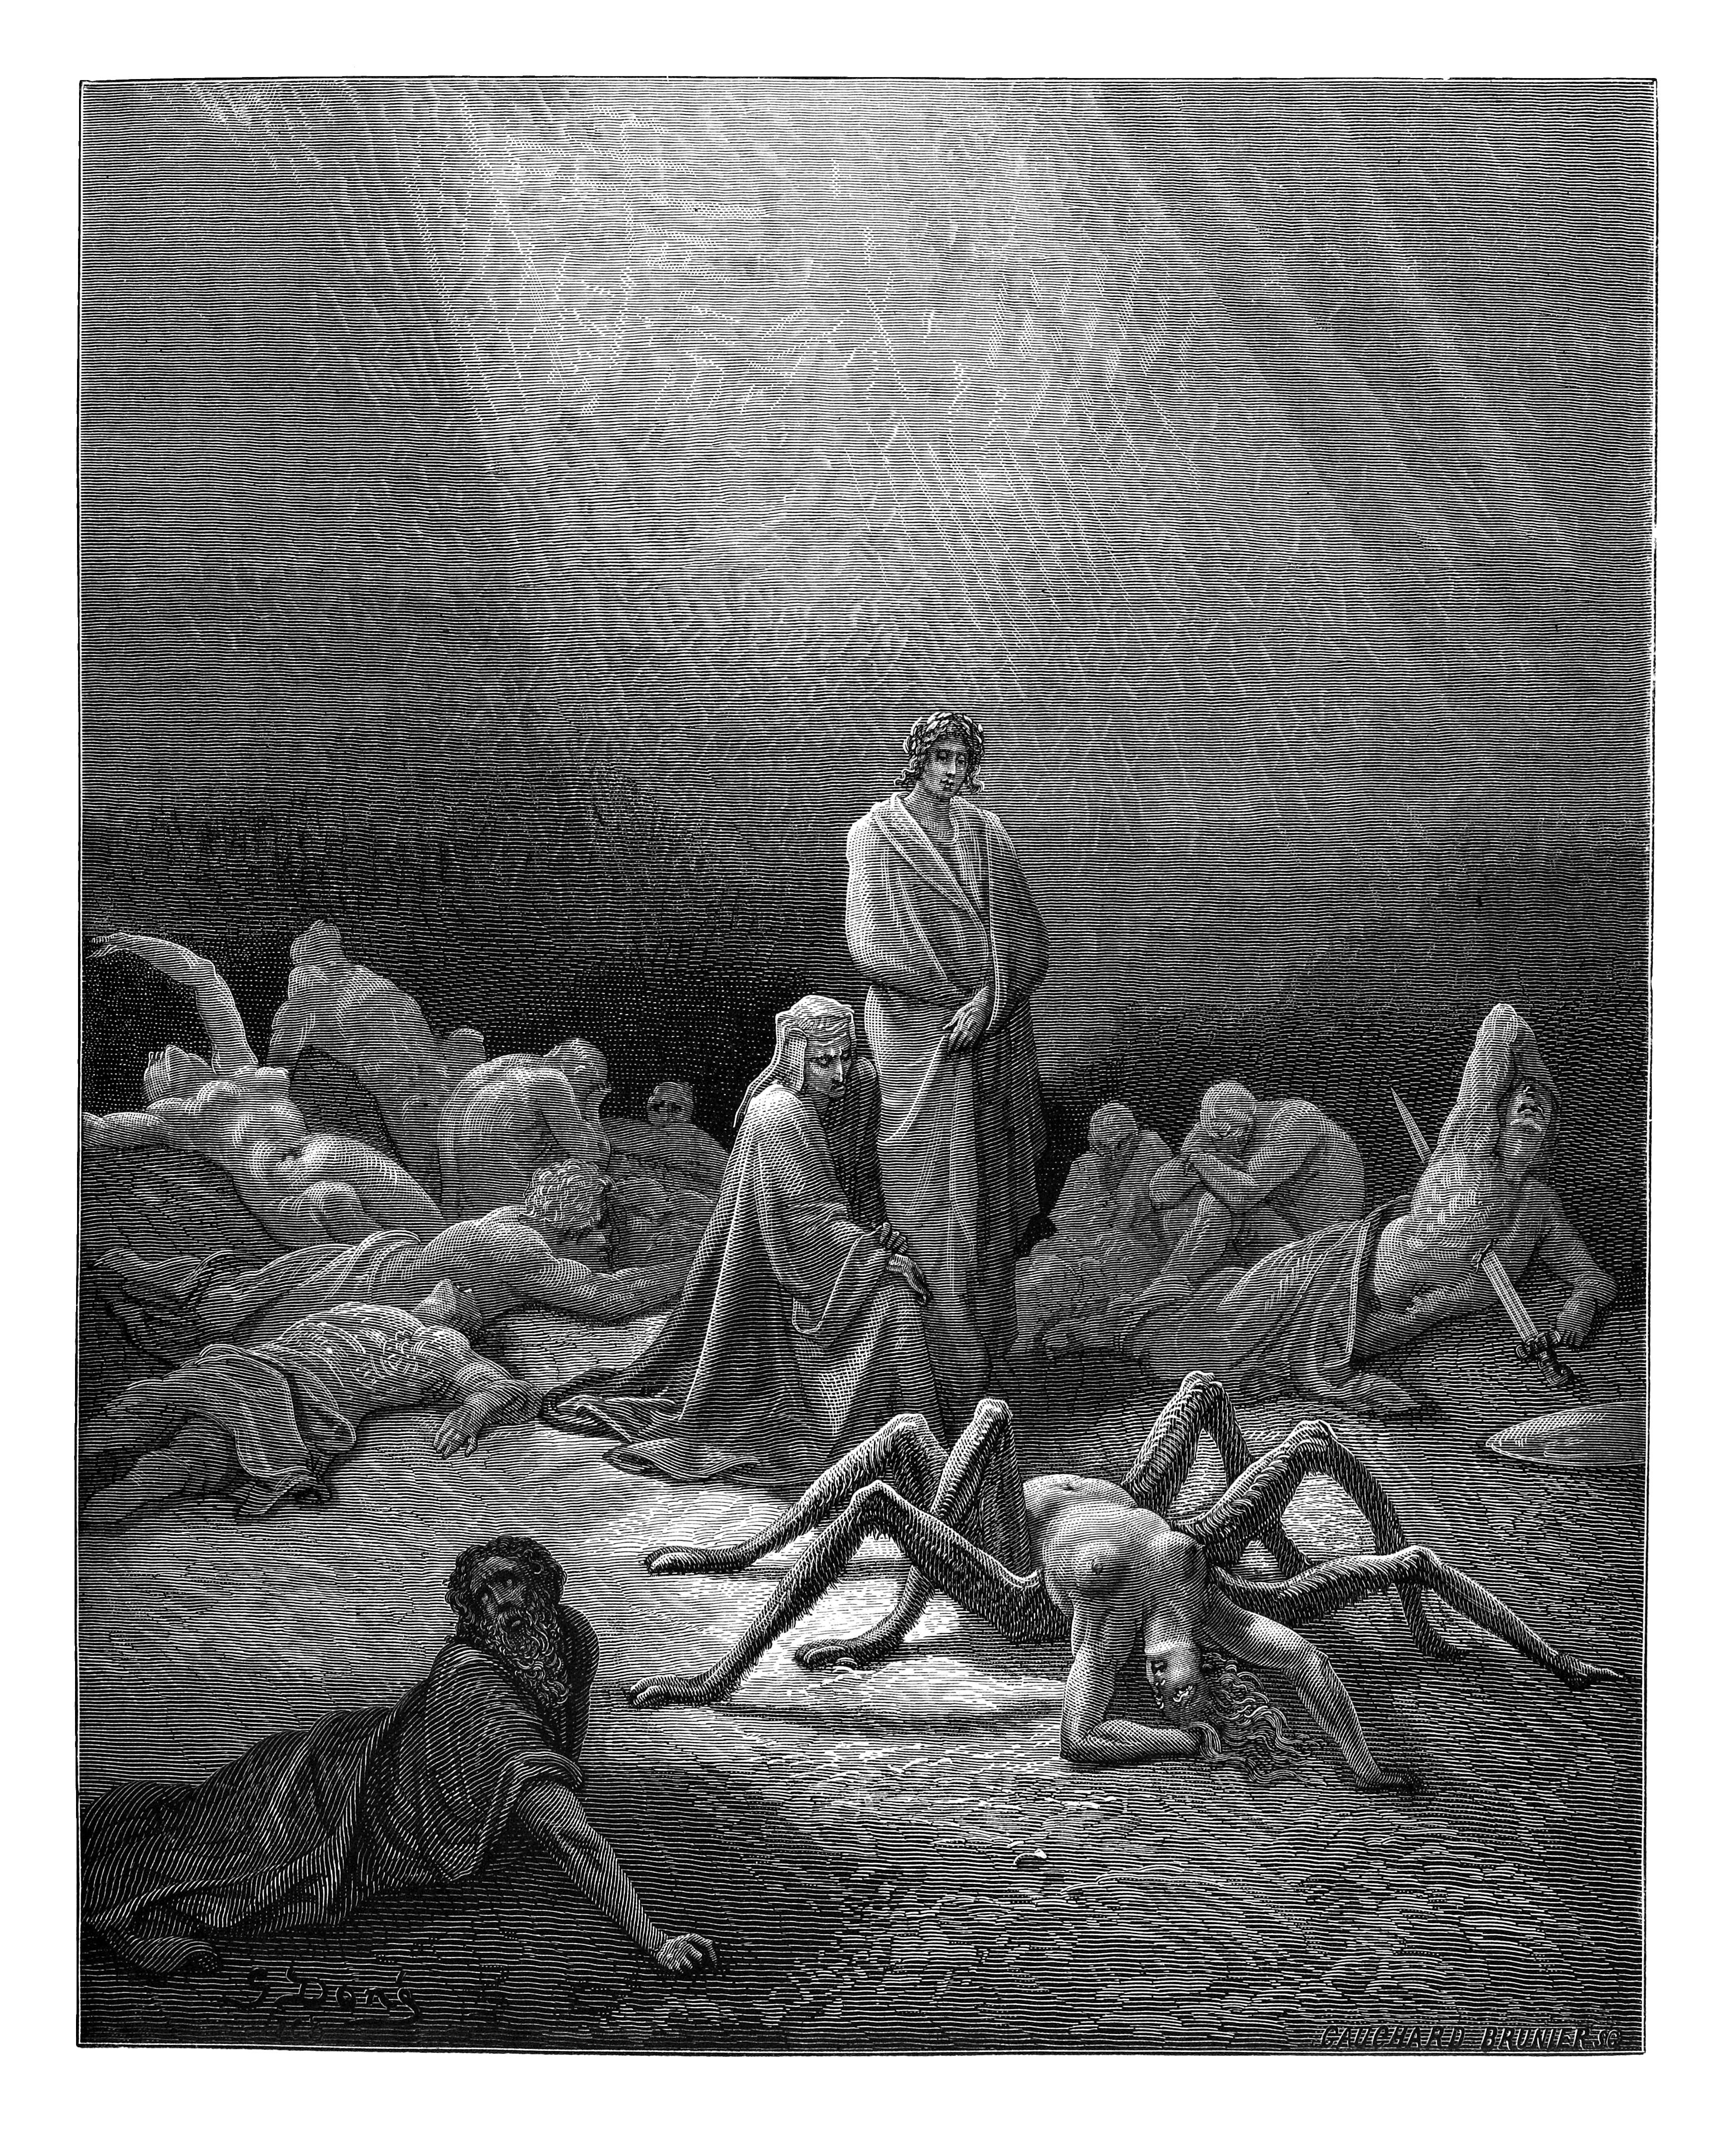
\includegraphics[height=\figsize]{illustrations/book_2/V02, c12.jpg}
\end{figure}

\begin{center}
\begin{minipage}{0.8\linewidth}
\textit{\\
"O folle Aragne, s\`{\i} vedea io te\\già mezza ragna, …"} \\
—V02, c12 \\~\\
\textit{"O fond Arachne! thee I also saw\\Half spider now …"} \\
—B02, c12
\end{minipage}
\end{center}

\newpage

\section{Canto 13(1)}

\begin{figure}[ht]
\centering
\includegraphics[height=\figsize]{illustrations/book_2/V02, c13(1).jpg}
\end{figure}

\begin{center}
\begin{minipage}{0.8\linewidth}
\textit{\\
"...vedrai gente innanzi a noi sedersi,\\e ciascuno è lungo la grotta assiso»."} \\
—V02, c13(1) \\~\\
\textit{"...thou shalt see\\A multitude before thee seated, each\\Along the shelving grot.\textquotesingle…"} \\
—B02, c13(1)
\end{minipage}
\end{center}

\newpage

\section{Canto 13(2)}

\begin{figure}[ht]
\centering
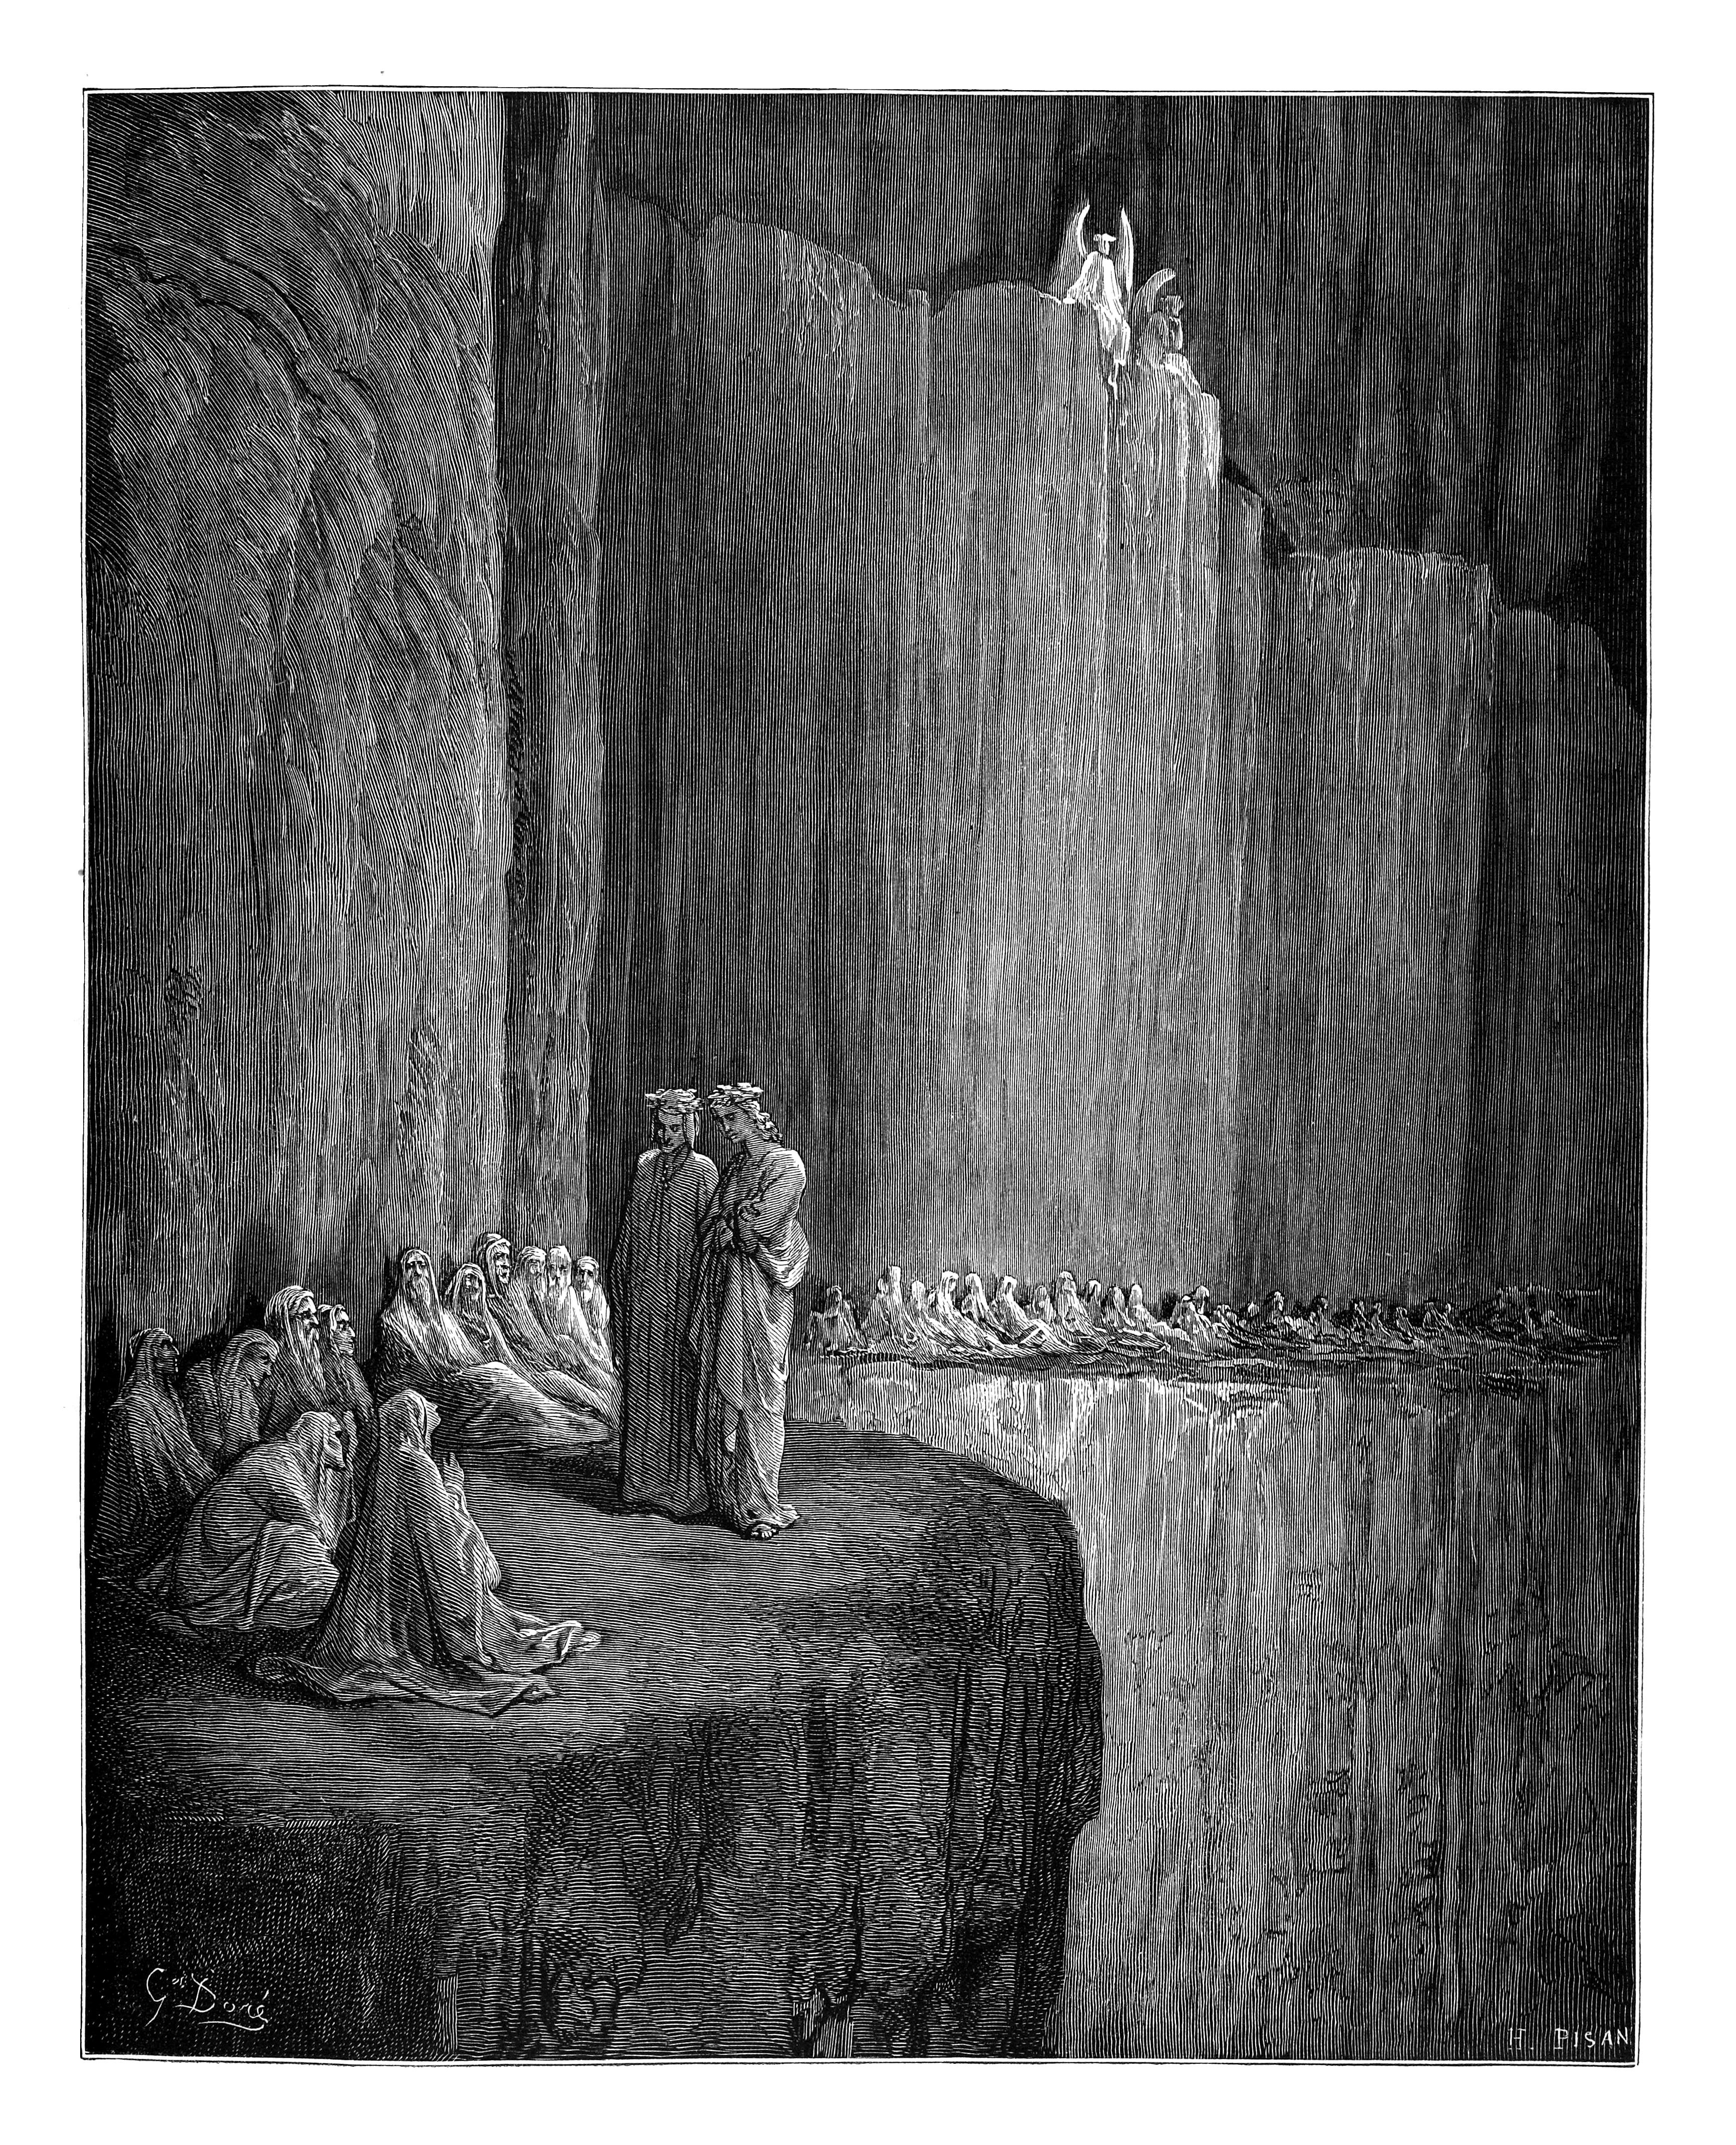
\includegraphics[height=\figsize]{illustrations/book_2/V02, c13(2).jpg}
\end{figure}

\begin{center}
\begin{minipage}{0.8\linewidth}
\textit{\\
"Savia non fui, avvegna che Sap\`{\i}a\\fossi chiamata, e fui de li altrui danni\\più lieta assai che di ventura mia."} \\
—V02, c13(2) \\~\\
\textit{"...Though Sapia nam'd\\In sapience I excell'd not, gladder far\\Of others' hurt, than of the good befell me."} \\
—B02, c13(2)
\end{minipage}
\end{center}

\newpage

\section{Canto 15}

\begin{figure}[ht]
\centering
\includegraphics[height=\figsize]{illustrations/book_2/V02, c15.jpg}
\end{figure}

\begin{center}
\begin{minipage}{0.8\linewidth}
\textit{\\
"...vidi genti accese in foco d’ira\\con pietre un giovinetto ancider, …"} \\
—V02, c15 \\~\\
\textit{"...I saw\\A multitude, in fury burning, slay\\With stones a stripling youth, …"} \\
—B02, c15
\end{minipage}
\end{center}

\newpage

\section{Canto 16(1)}

\begin{figure}[ht]
\centering
\includegraphics[height=\figsize]{illustrations/book_2/V02, c16(1).jpg}
\end{figure}

\begin{center}
\begin{minipage}{0.8\linewidth}
\textit{\\
"...tu chi se’ che ’l nostro fummo fendi,"} \\
—V02, c16(1) \\~\\
\textit{"...who art thou, that through our smoke dost\\cleave?..."} \\
—B02, c16(1)
\end{minipage}
\end{center}

\newpage

\section{Canto 16(2)}

\begin{figure}[ht]
\centering
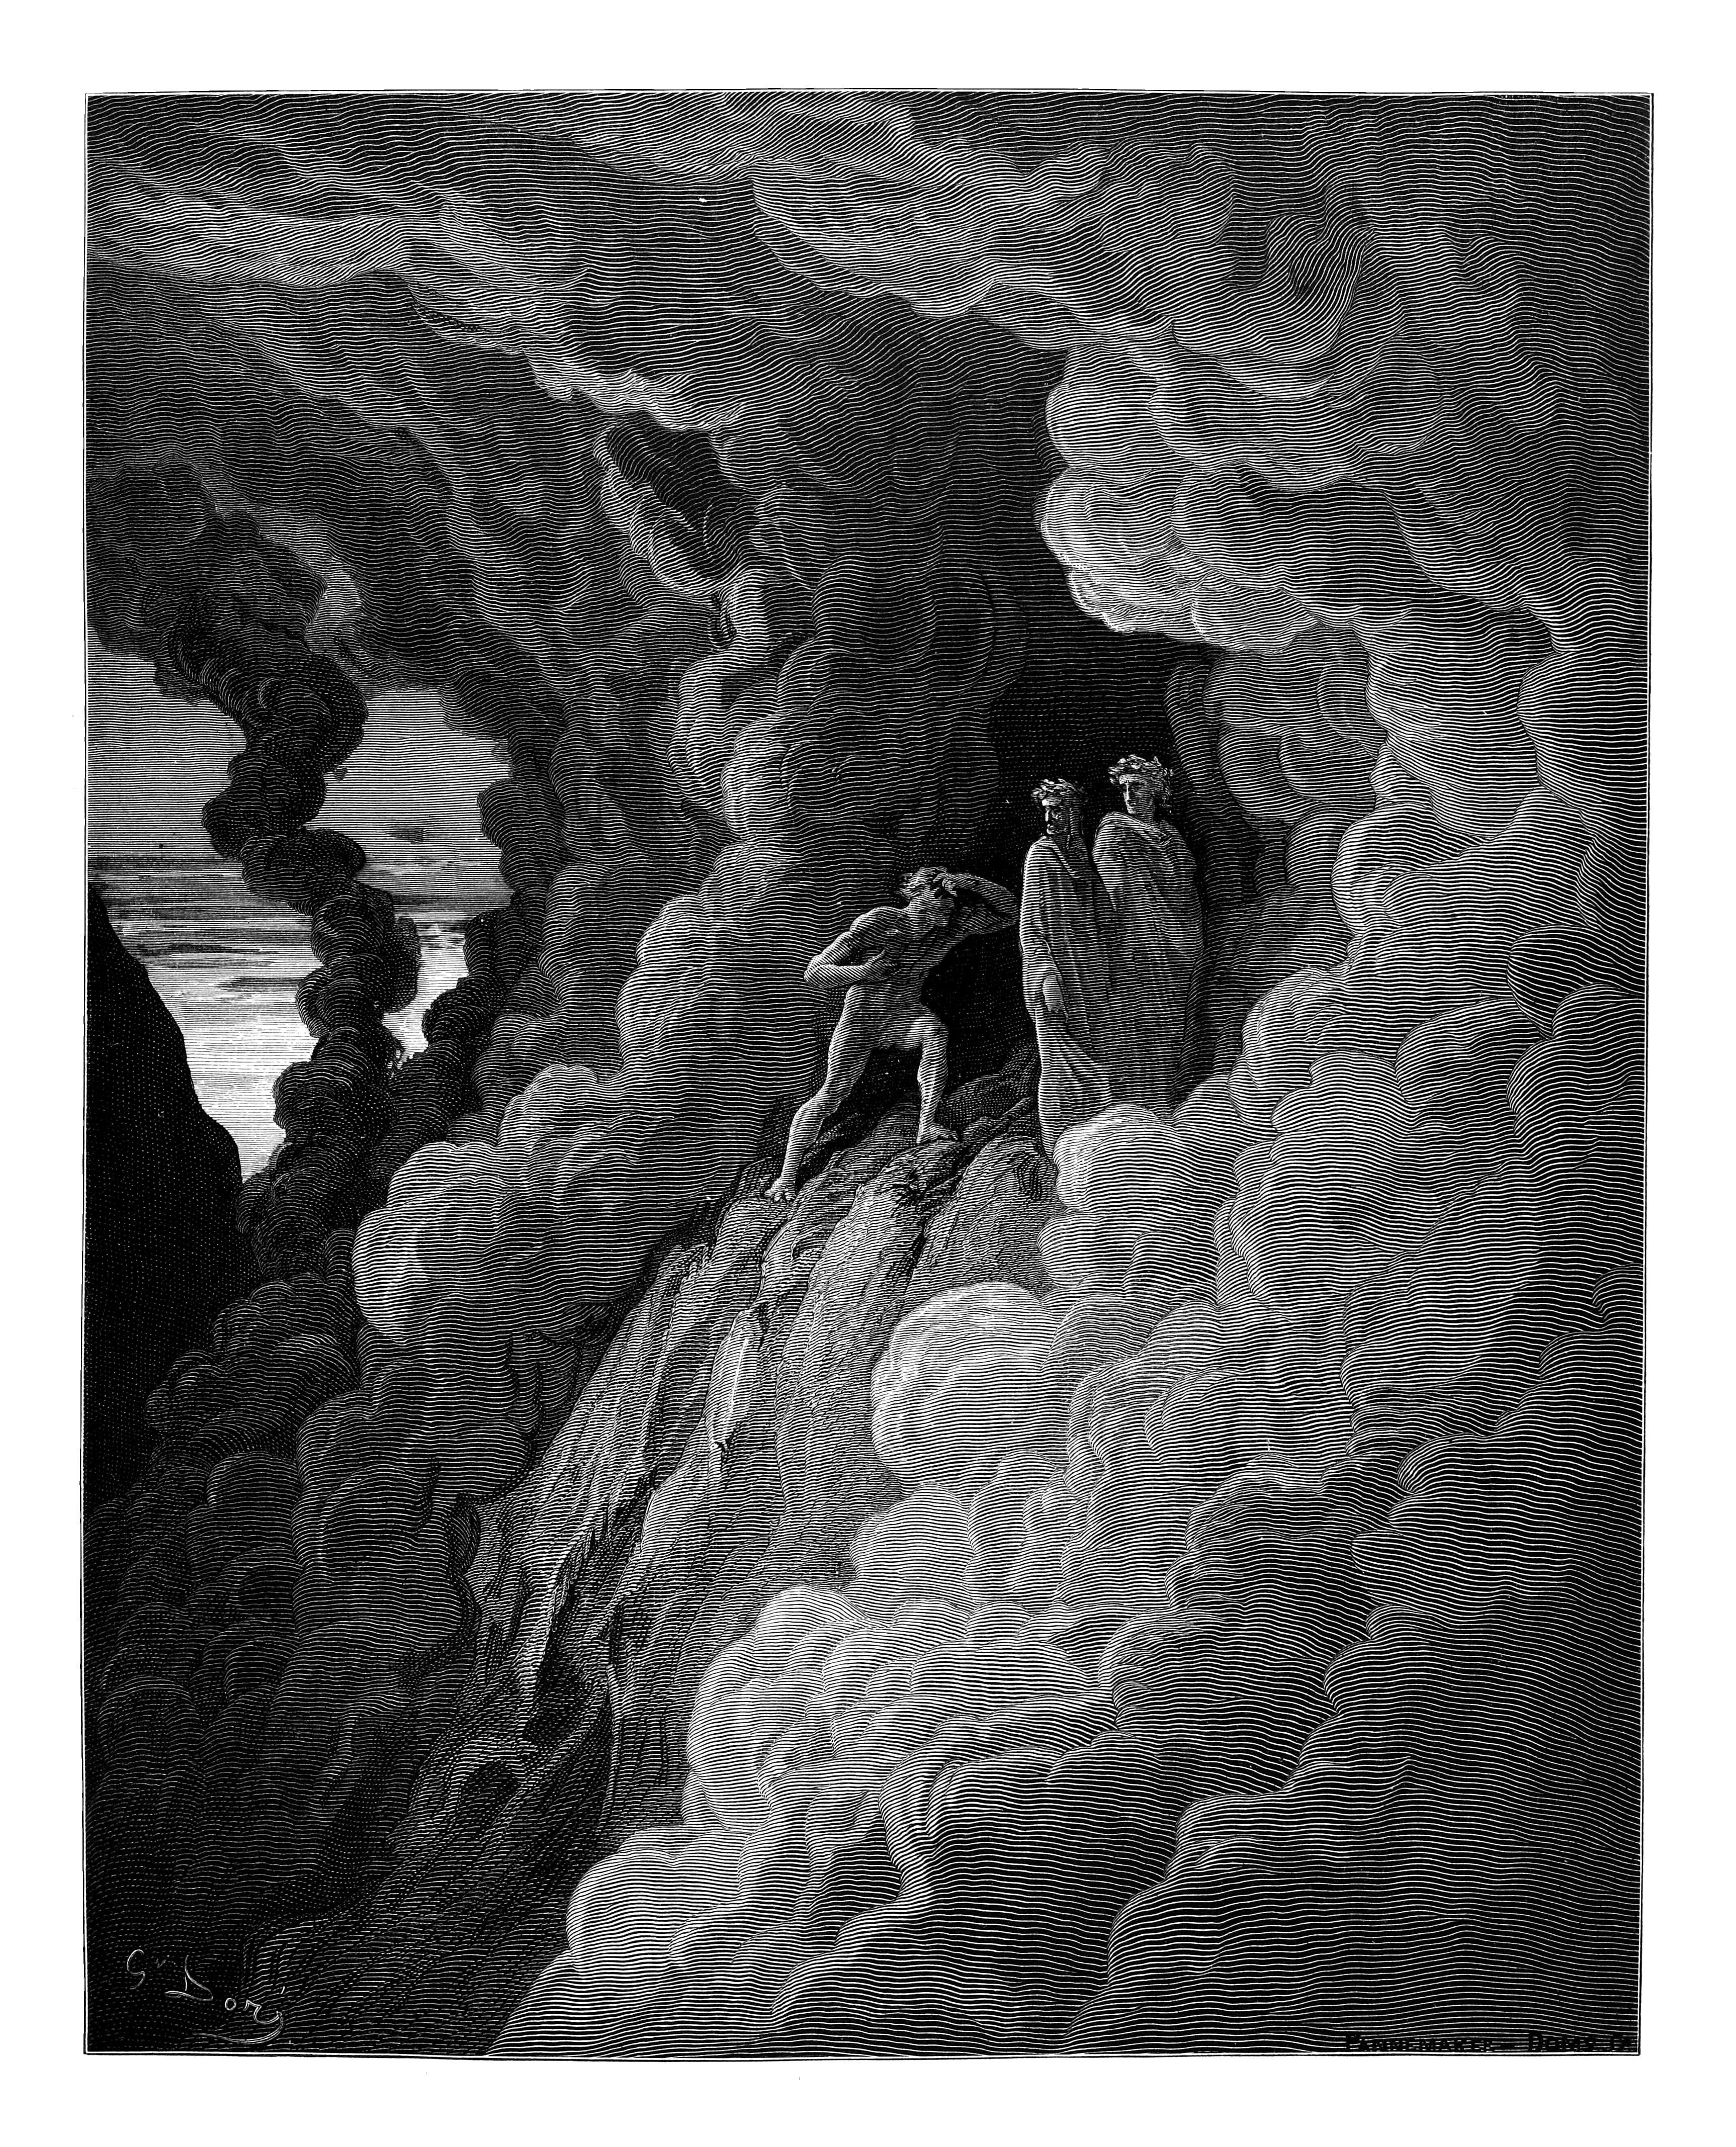
\includegraphics[height=\figsize]{illustrations/book_2/V02, c16(2).jpg}
\end{figure}

\begin{center}
\begin{minipage}{0.8\linewidth}
\textit{\\
"Vedi l’albor che per lo fummo raia\\già biancheggiare, …"} \\
—V02, c16(2) \\~\\
\textit{"...Behold\\The dawn with white ray glimm'ring through the mist."} \\
—B02, c16(2)
\end{minipage}
\end{center}

\newpage

\section{Canto 18}

\begin{figure}[ht]
\centering
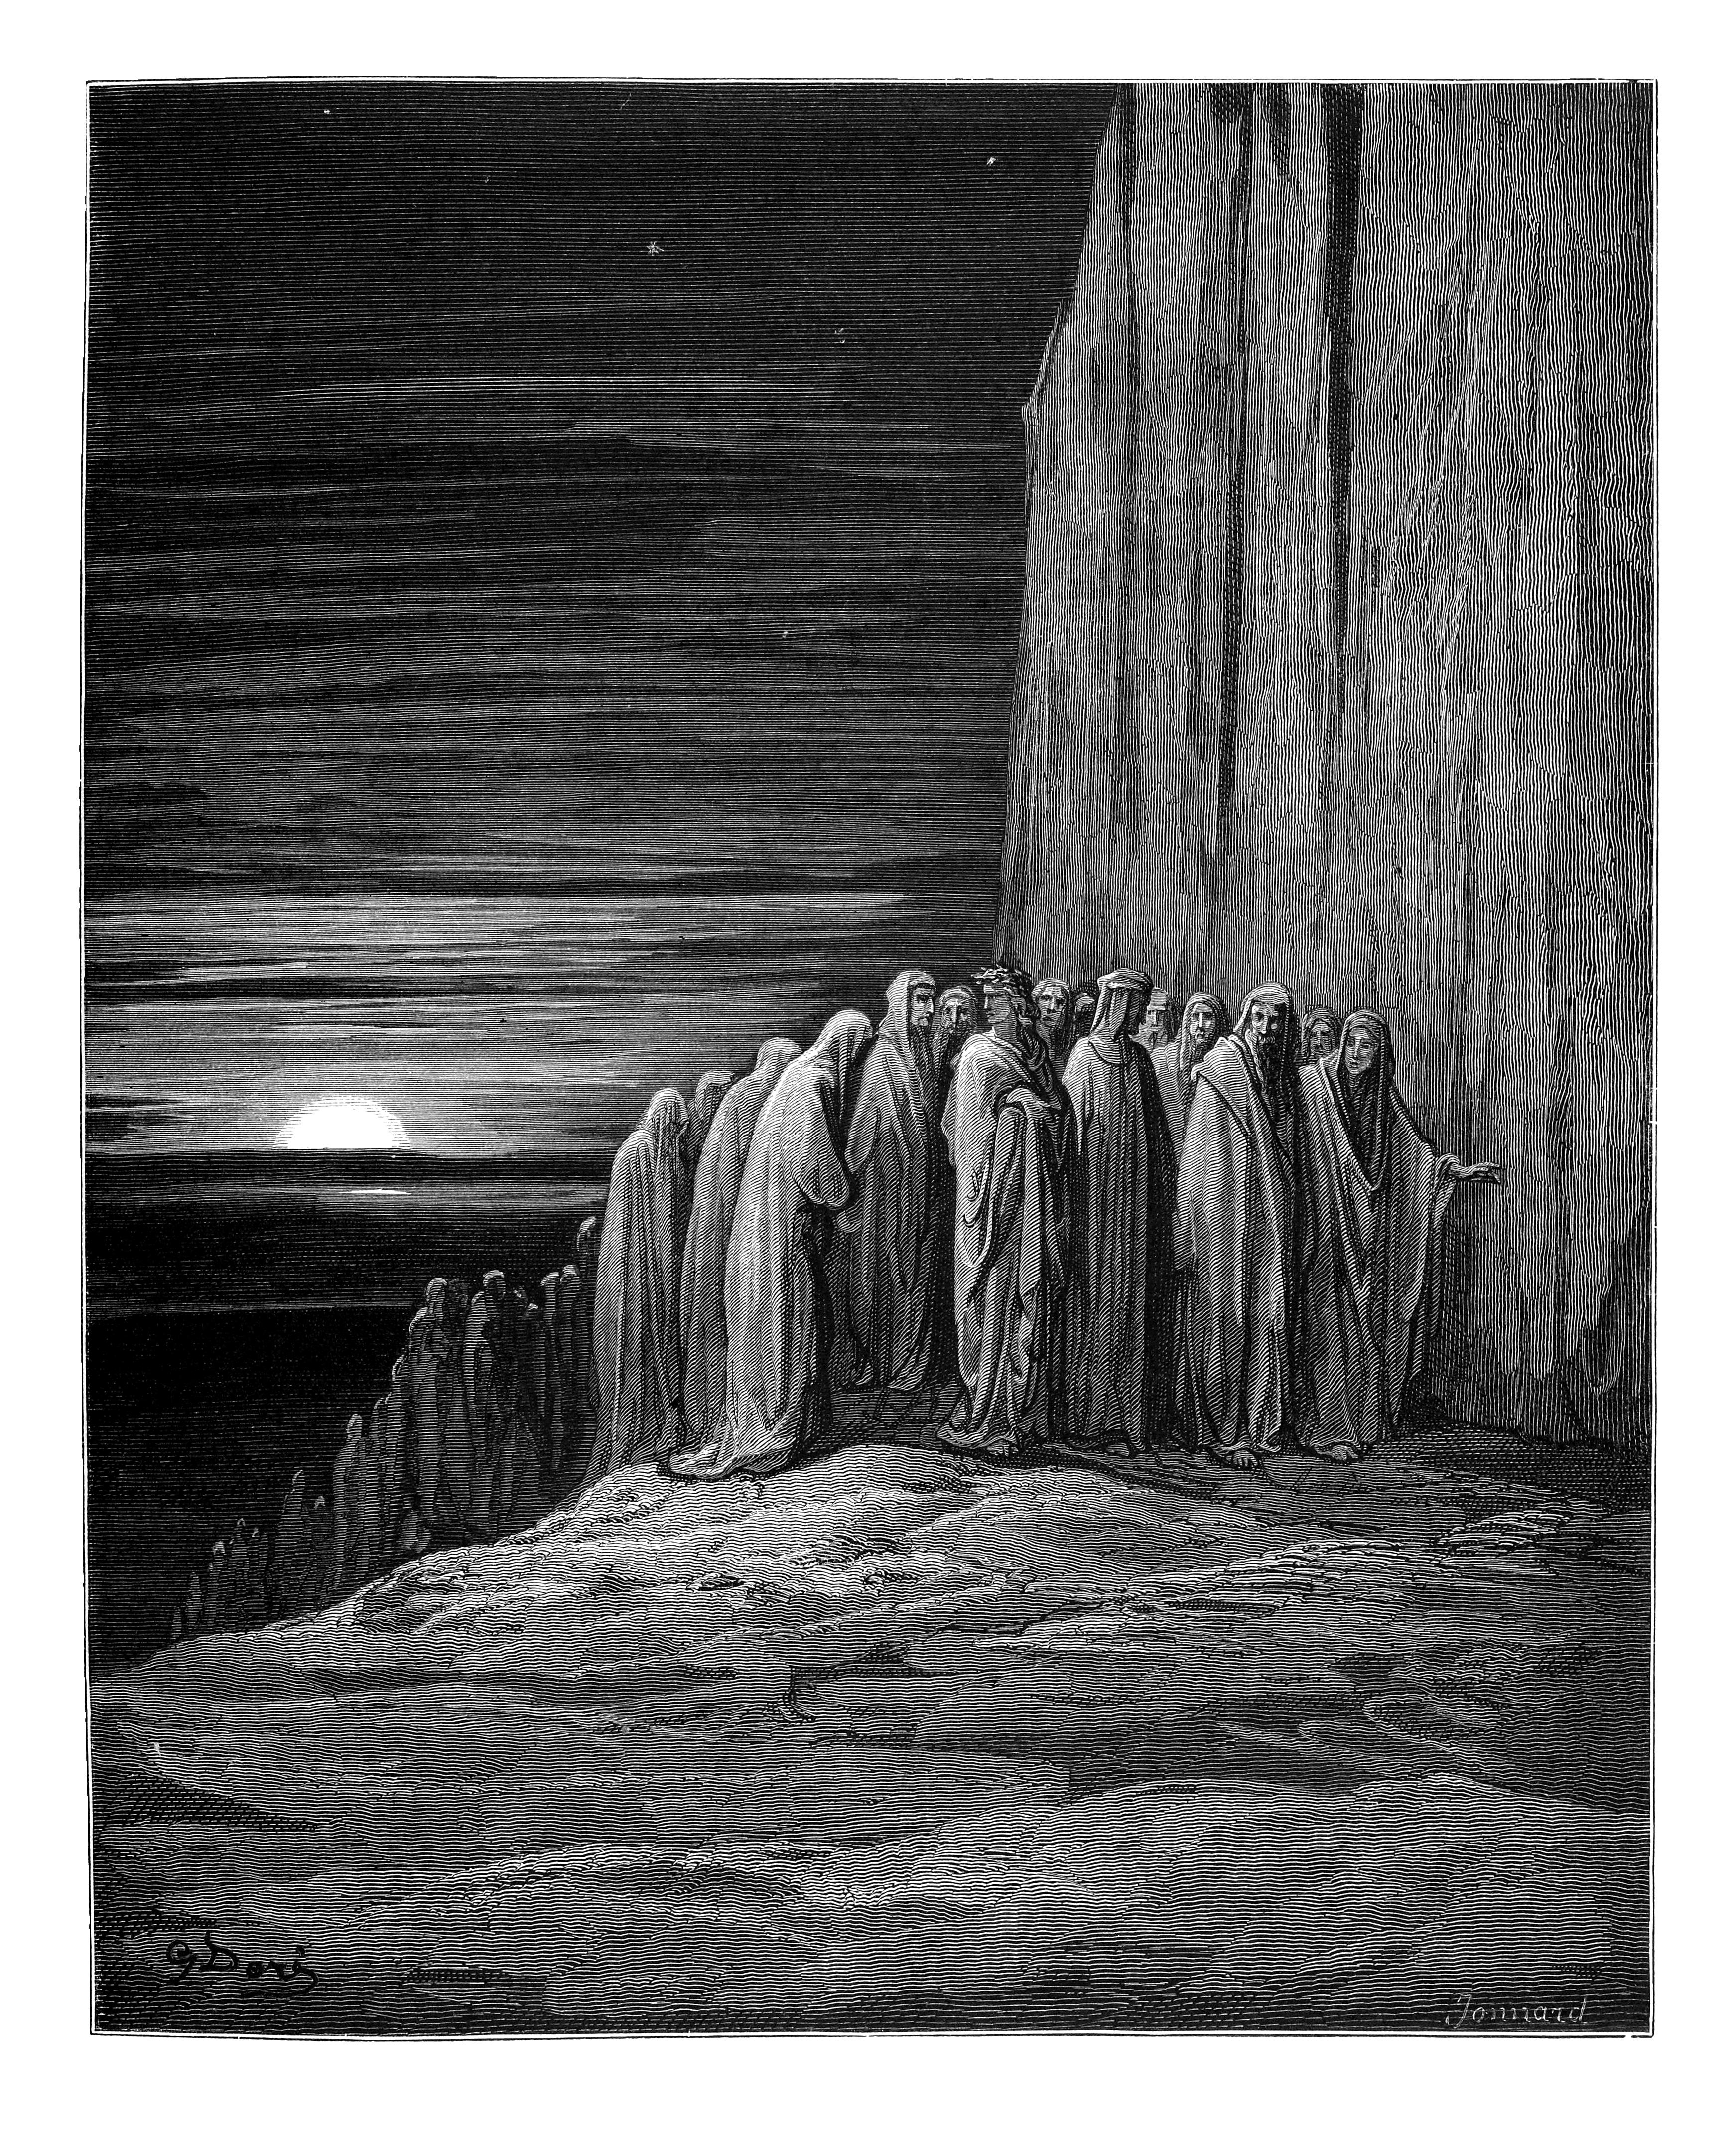
\includegraphics[height=\figsize]{illustrations/book_2/V02, c18.jpg}
\end{figure}

\begin{center}
\begin{minipage}{0.8\linewidth}
\textit{\\
"...studio di ben far grazia rinverda»."} \\
—V02, c18 \\~\\
\textit{"...Hearty zeal\\To serve reanimates celestial grace.\textquotesingle"} \\
—B02, c18
\end{minipage}
\end{center}

\newpage

\section{Canto 19(1)}

\begin{figure}[ht]
\centering
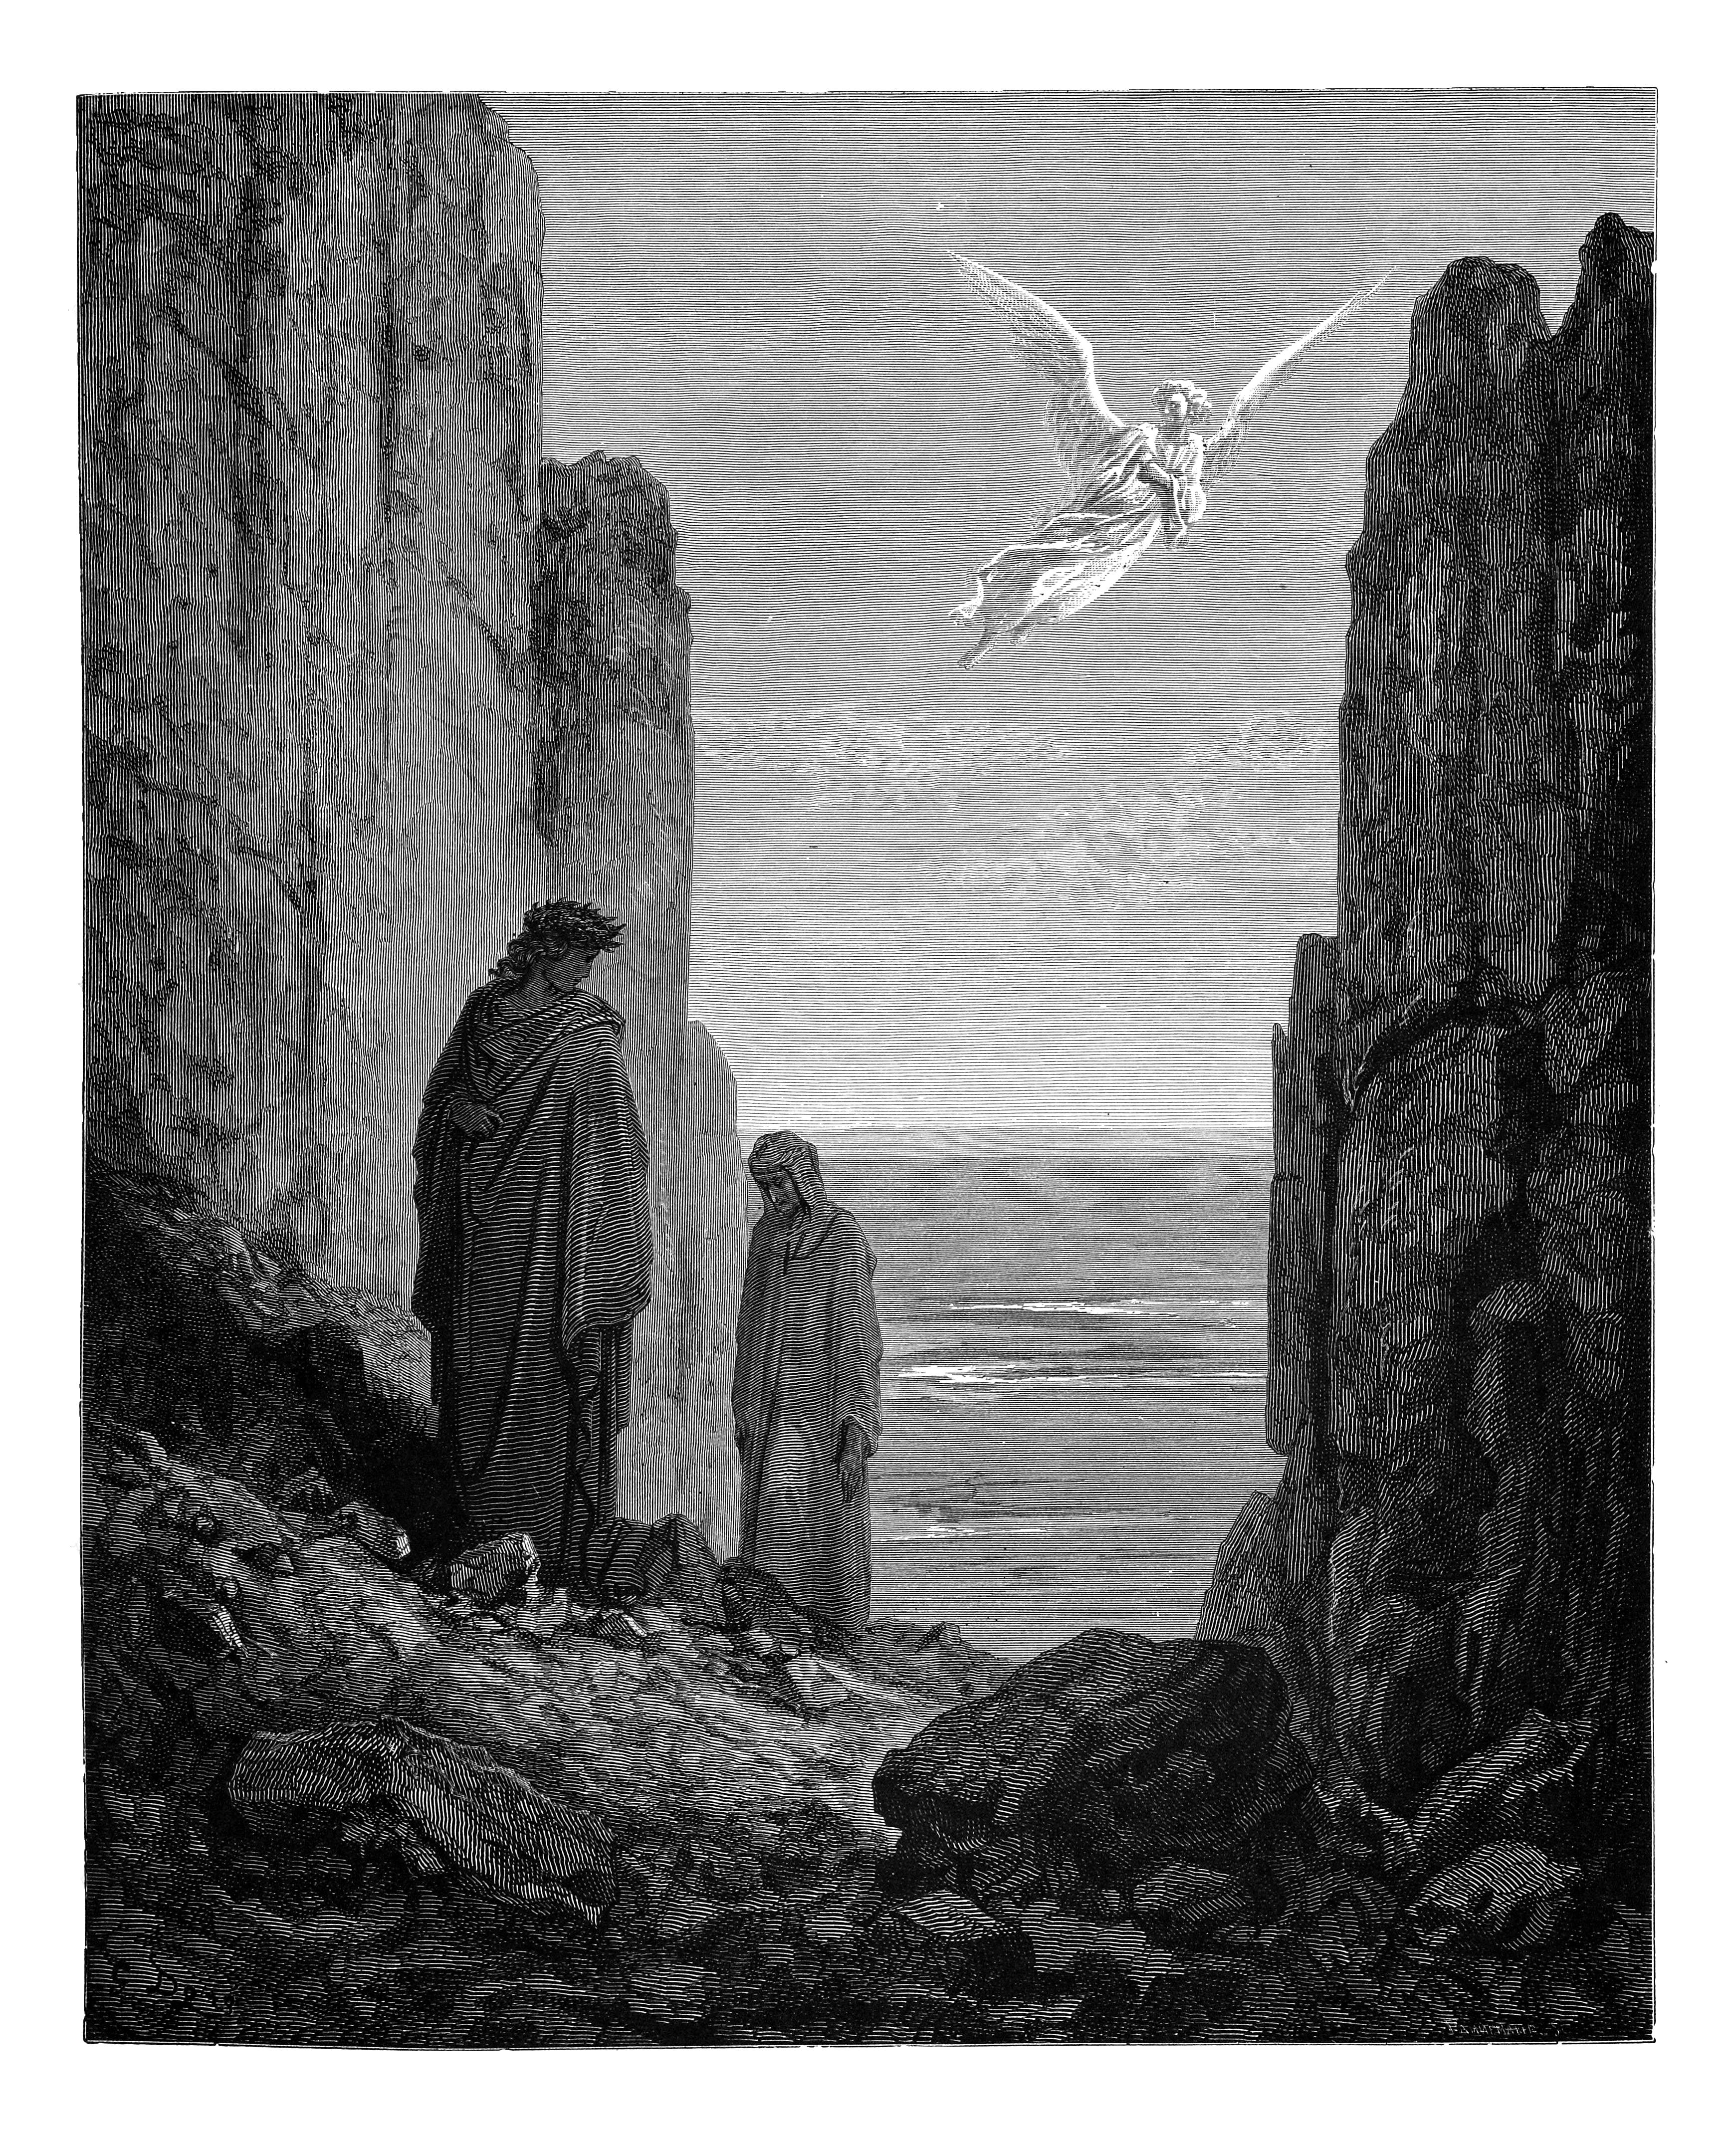
\includegraphics[height=\figsize]{illustrations/book_2/V02, c19(1).jpg}
\end{figure}

\begin{center}
\begin{minipage}{0.8\linewidth}
\textit{\\
"Seguendo lui, portava la mia fronte\\come colui che l’ha di pensier carca,"} \\
—V02, c19(1) \\~\\
\textit{"...I follow' d, stooping low\\My forehead, as a man, o'ercharg'd with thought,"} \\
—B02, c19(1)
\end{minipage}
\end{center}

\newpage

\section{Canto 19(2)}

\begin{figure}[ht]
\centering
\includegraphics[height=\figsize]{illustrations/book_2/V02, c19(2).jpg}
\end{figure}

\begin{center}
\begin{minipage}{0.8\linewidth}
\textit{\\
"S\`{\i} come l’occhio nostro non s’aderse\\in alto, fisso a le cose terrene,\\cos\`{\i} giustizia qui a terra il merse."} \\
—V02, c19(2) \\~\\
\textit{"...E'en as our eyes\\Fasten'd below, nor e'er to loftier clime\\Were lifted, thus hath justice level'd us\\Here on the earth. …"} \\
—B02, c19(2)
\end{minipage}
\end{center}

\newpage

\section{Canto 20}

\begin{figure}[ht]
\centering
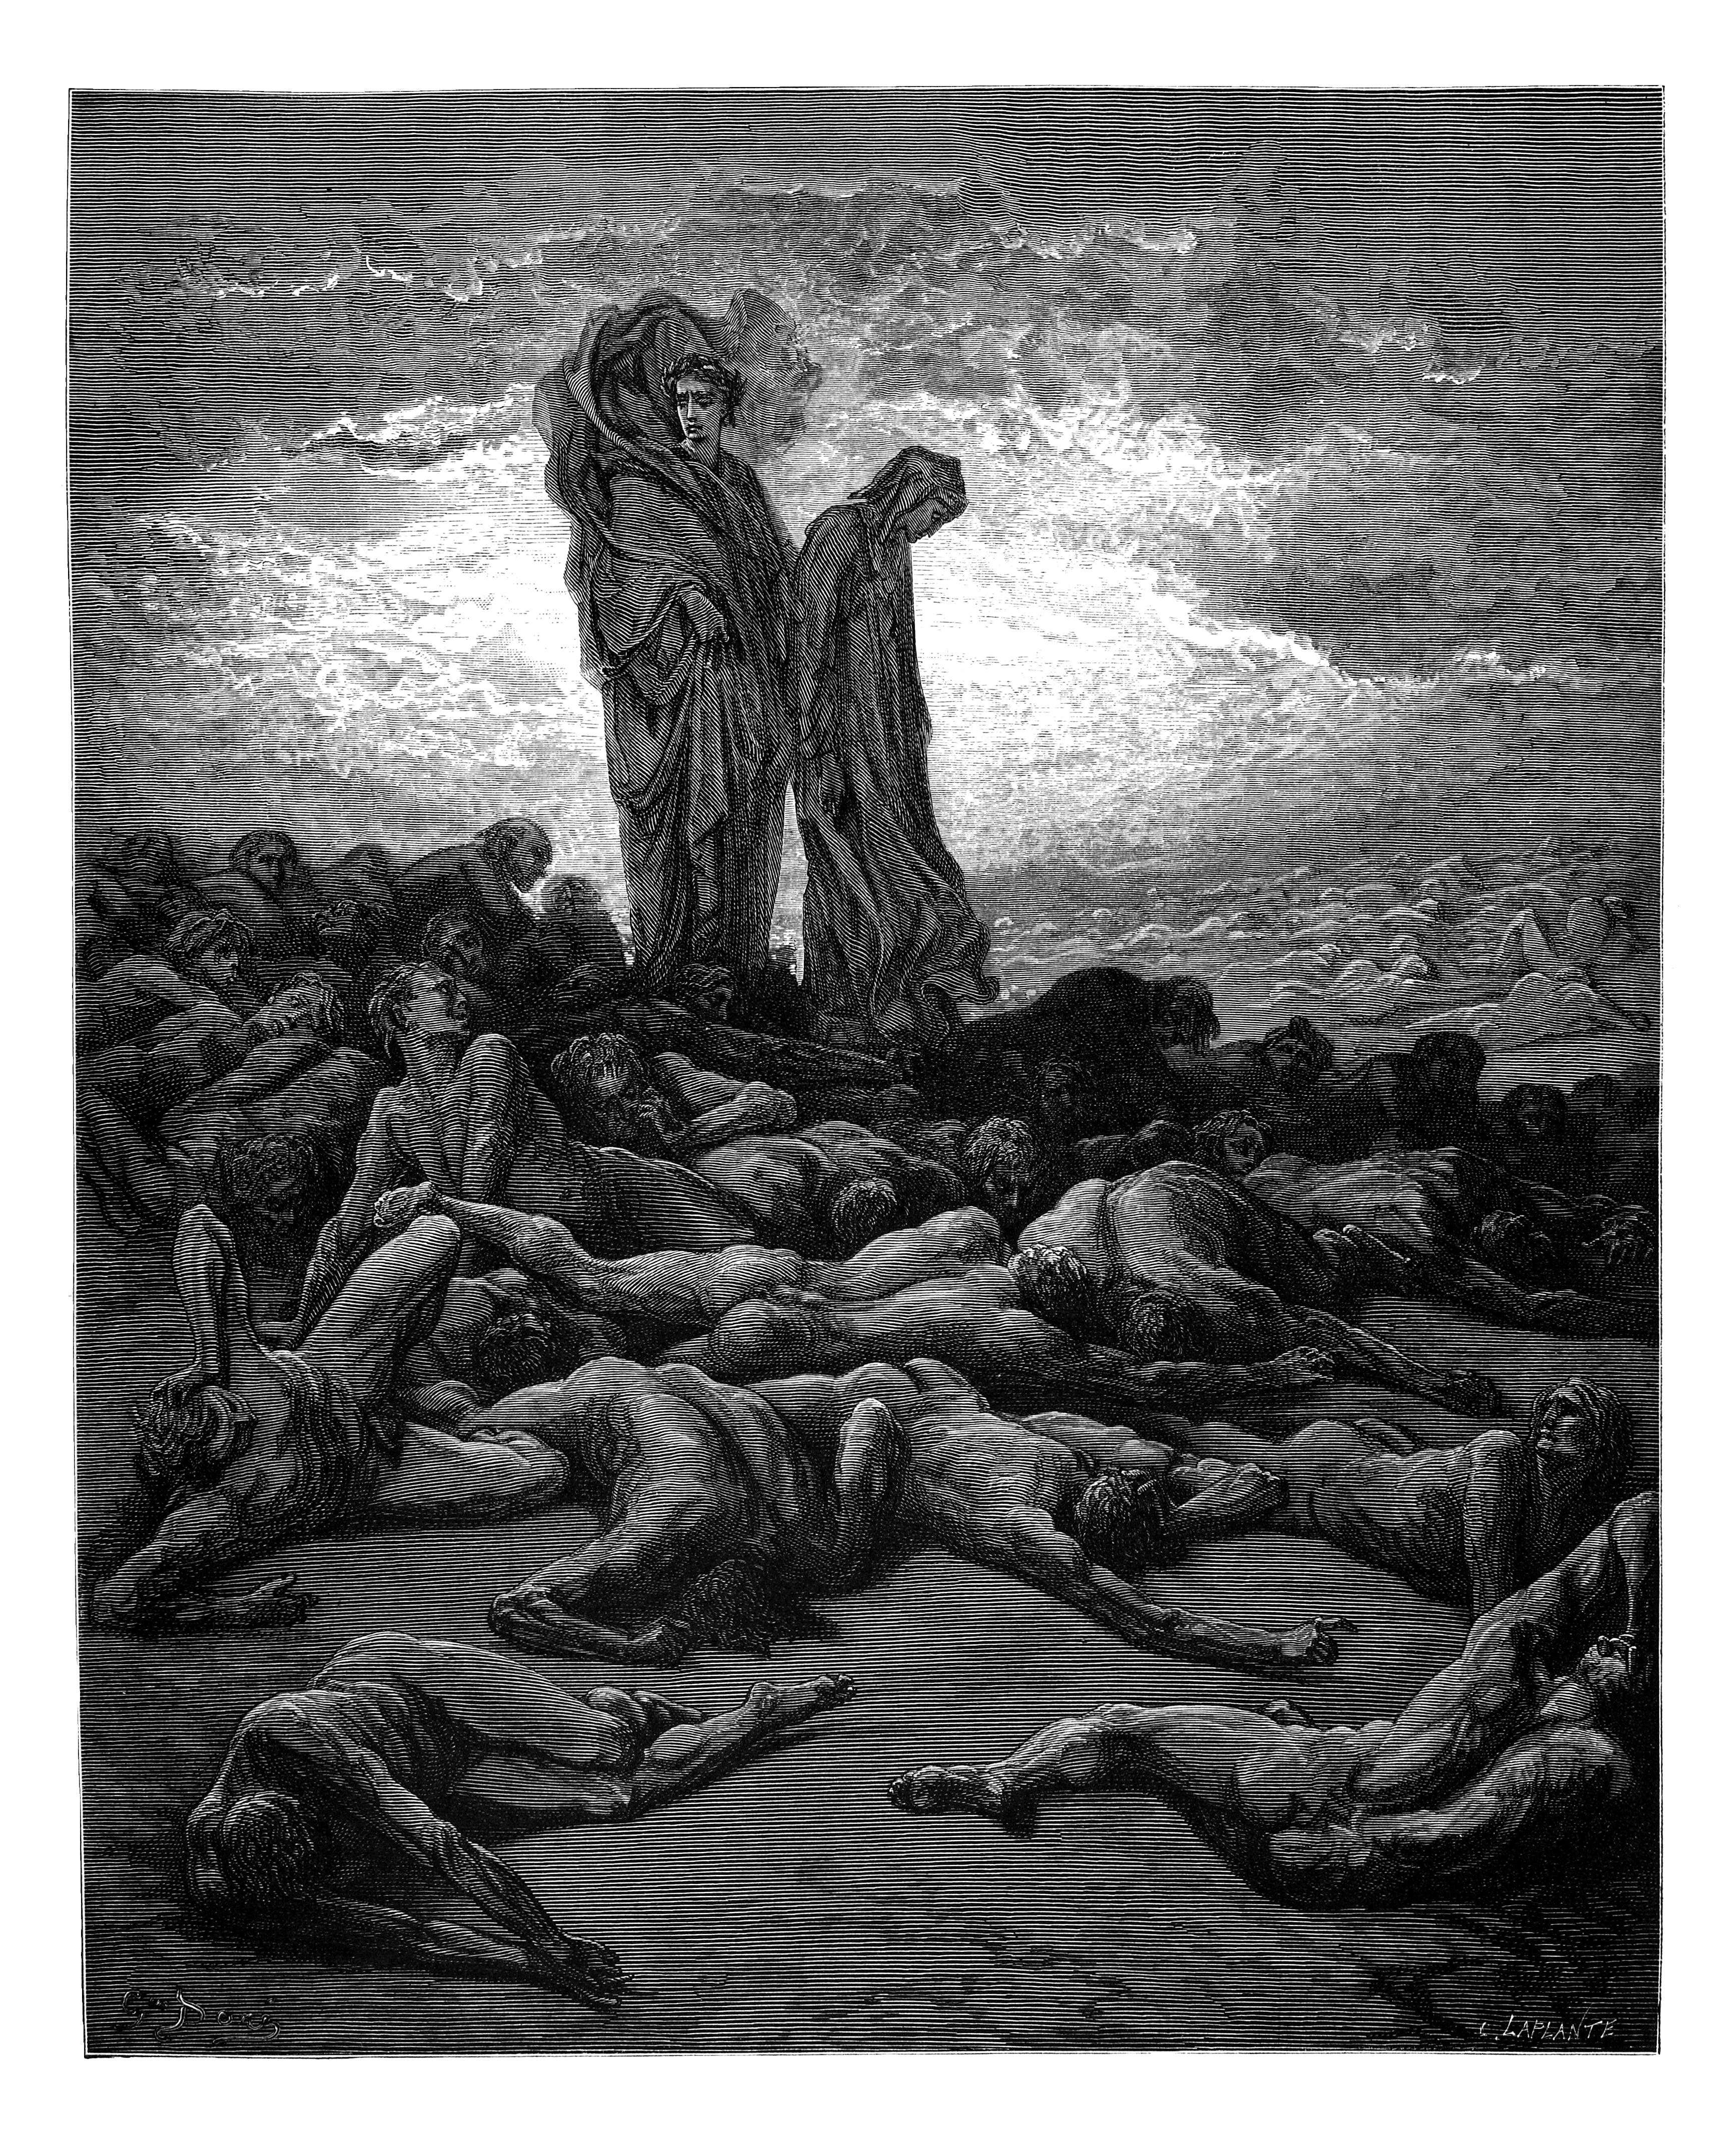
\includegraphics[height=\figsize]{illustrations/book_2/V02, c20.jpg}
\end{figure}

\begin{center}
\begin{minipage}{0.8\linewidth}
\textit{\\
"No’ istavamo immobili e sospesi\\come i pastor che prima udir quel canto,"} \\
—V02, c20 \\~\\
\textit{"...We stood\\Immovably suspended, like to those,\\The shepherds, who first heard in Bethlehem's field\\That song: ..."} \\
—B02, c20
\end{minipage}
\end{center}

\newpage

\section{Canto 23}

\begin{figure}[ht]
\centering
\includegraphics[height=\figsize]{illustrations/book_2/V02, c23.jpg}
\end{figure}

\begin{center}
\begin{minipage}{0.8\linewidth}
\textit{\\
"...ecco del profondo de la testa\\volse a me li occhi un’ombra e guard\`o fiso;"} \\
—V02, c23 \\~\\
\textit{"...lo! a spirit turn'd his eyes\\In their deep-sunken cell, and fasten'd them\\On me, …"} \\
—B02, c23
\end{minipage}
\end{center}

\newpage

\section{Canto 24(1)}

\begin{figure}[ht]
\centering
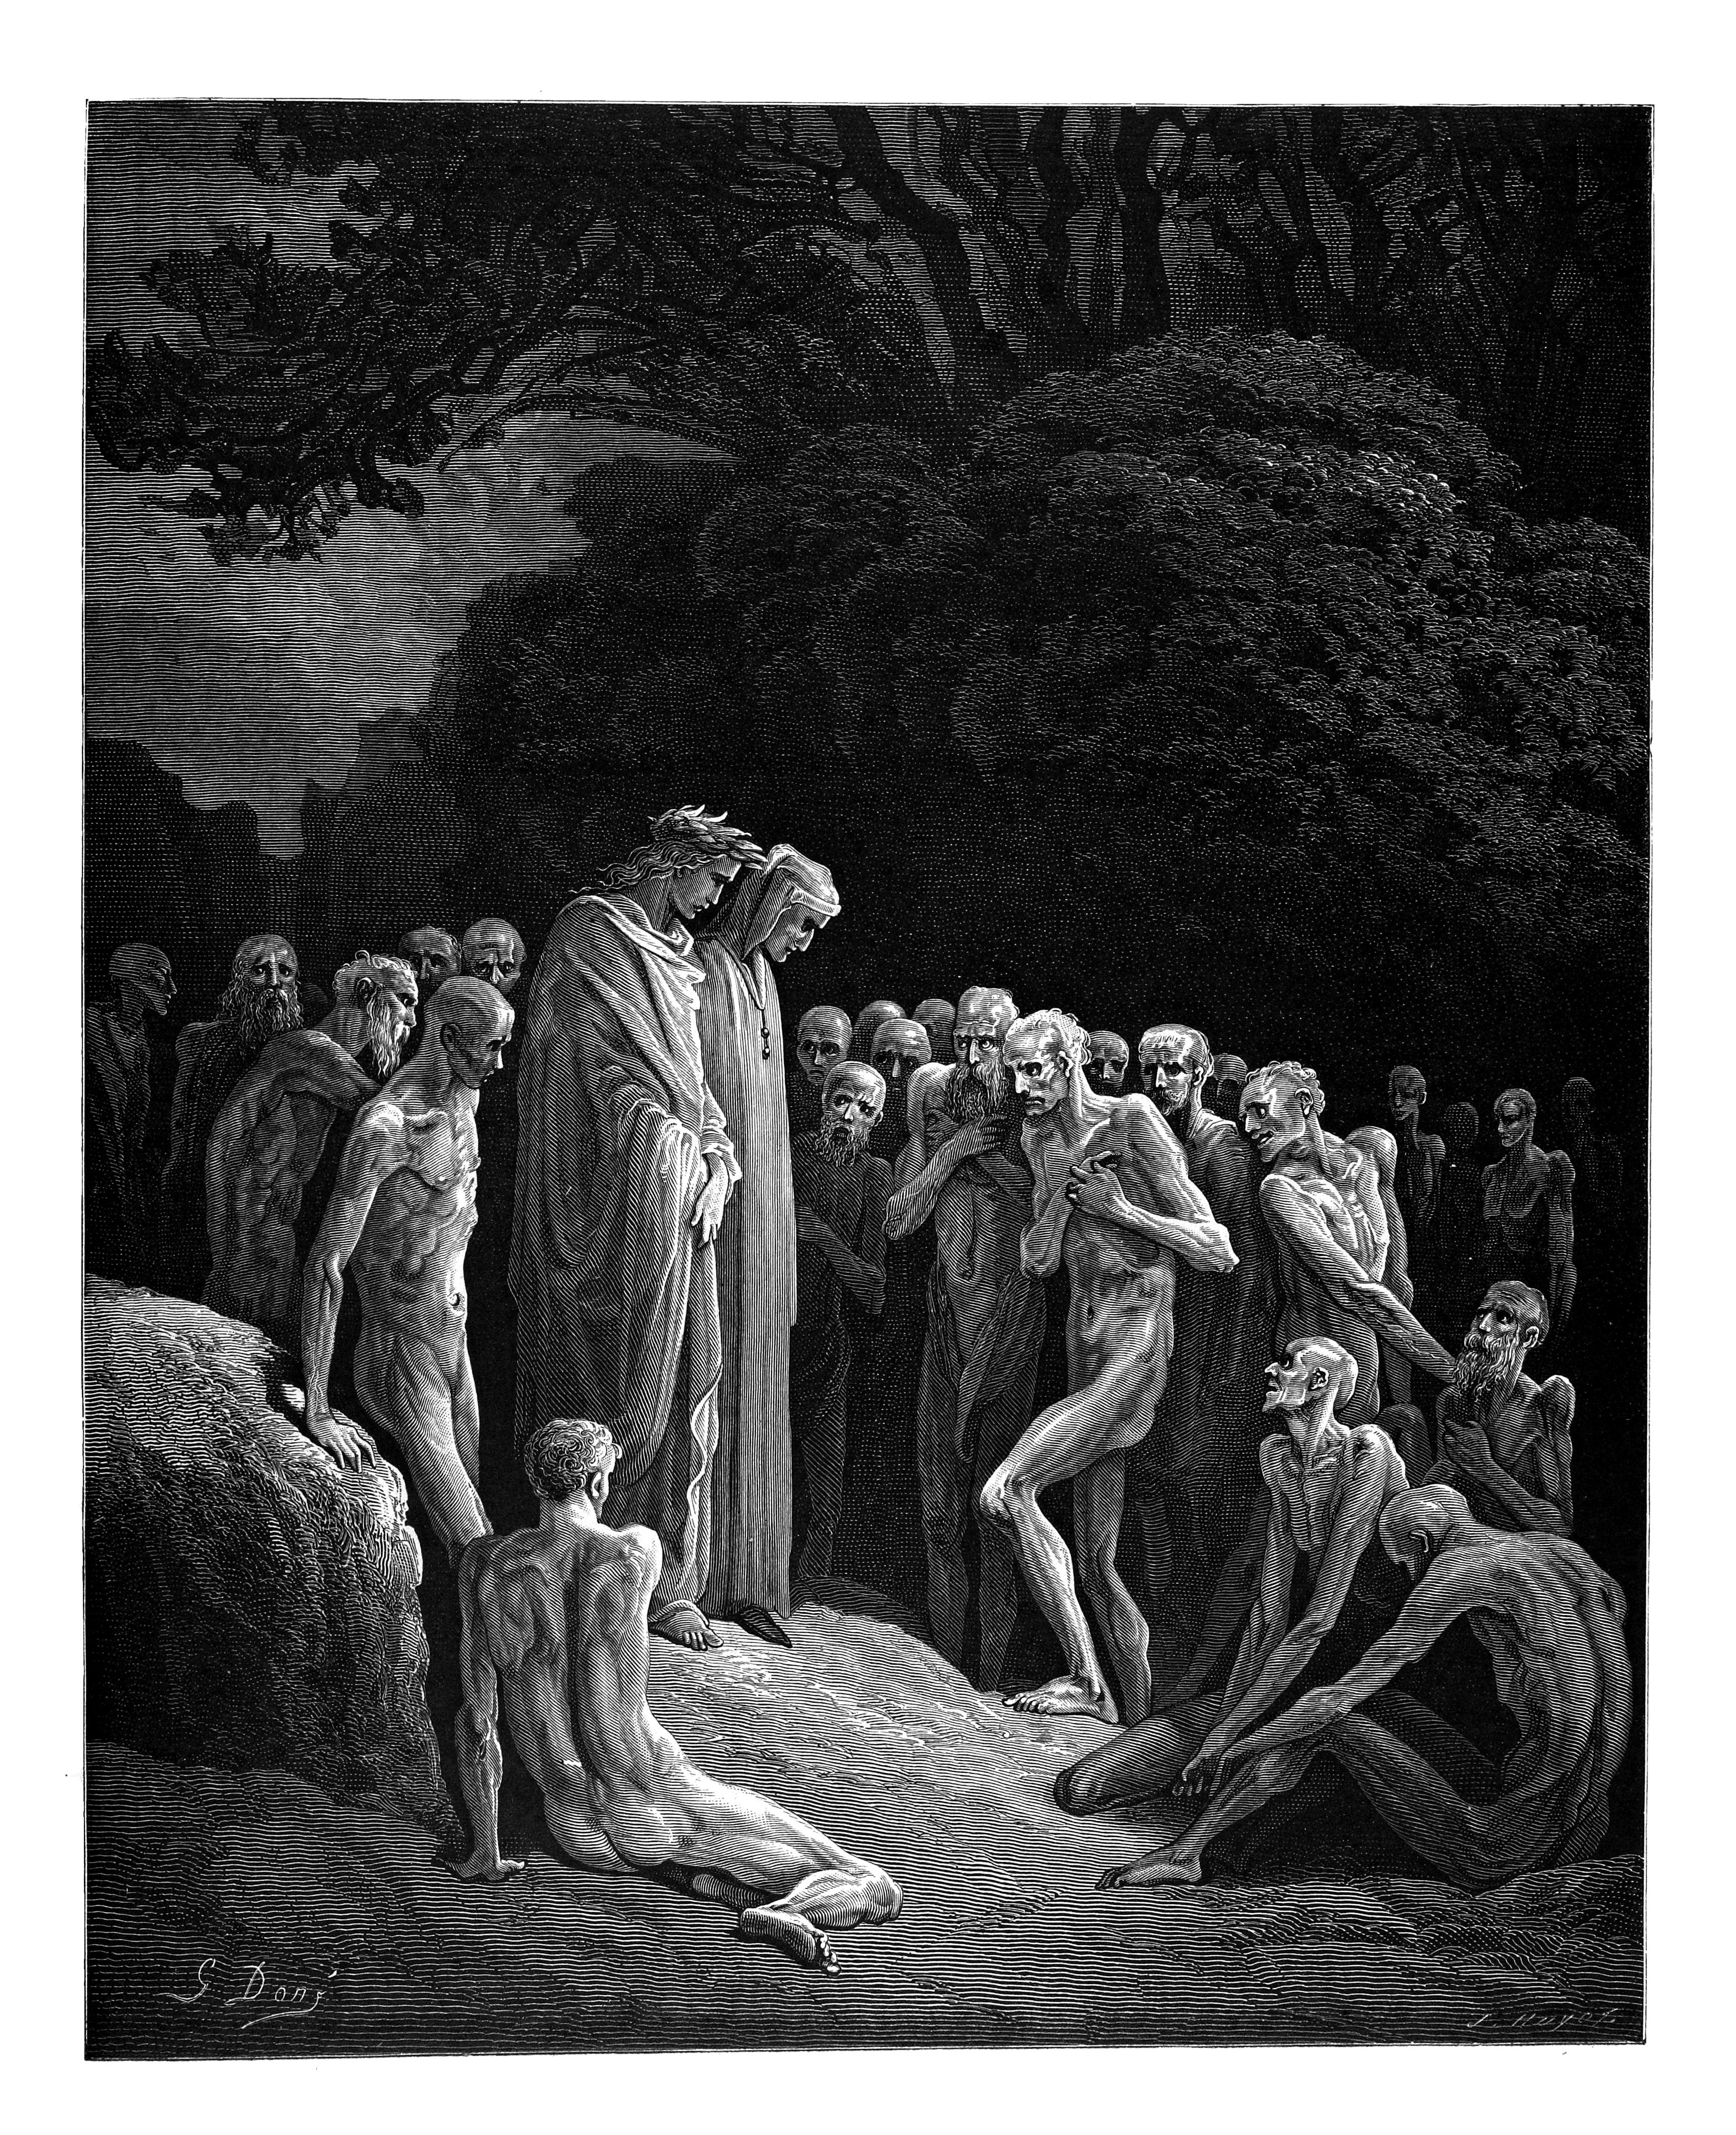
\includegraphics[height=\figsize]{illustrations/book_2/V02, c24(1).jpg}
\end{figure}

\begin{center}
\begin{minipage}{0.8\linewidth}
\textit{\\
"...l’ombre, che parean cose rimorte,\\per le fosse de li occhi ammirazione\\traean di me, di mio vivere accorte."} \\
—V02, c24(1) \\~\\
\textit{"...The shadowy forms,\\That seem'd things dead and dead again, drew in\\At their deep-delved orbs rare wonder of me,\\Perceiving I had life; …"} \\
—B02, c24(1)
\end{minipage}
\end{center}

\newpage

\section{Canto 24(2)}

\begin{figure}[ht]
\centering
\includegraphics[height=\figsize]{illustrations/book_2/V02, c24(2).jpg}
\end{figure}

\begin{center}
\begin{minipage}{0.8\linewidth}
\textit{\\
"Vidi gente sott’esso alzar le mani\\e gridar non so che verso le fronde,"} \\
—V02, c24(2) \\~\\
\textit{"Beneath it were a multitude, that rais'd\\Their hands, and shouted forth I know not What\\Unto the boughs; …"} \\
—B02, c24(2)
\end{minipage}
\end{center}

\newpage

\section{Canto 25}

\begin{figure}[ht]
\centering
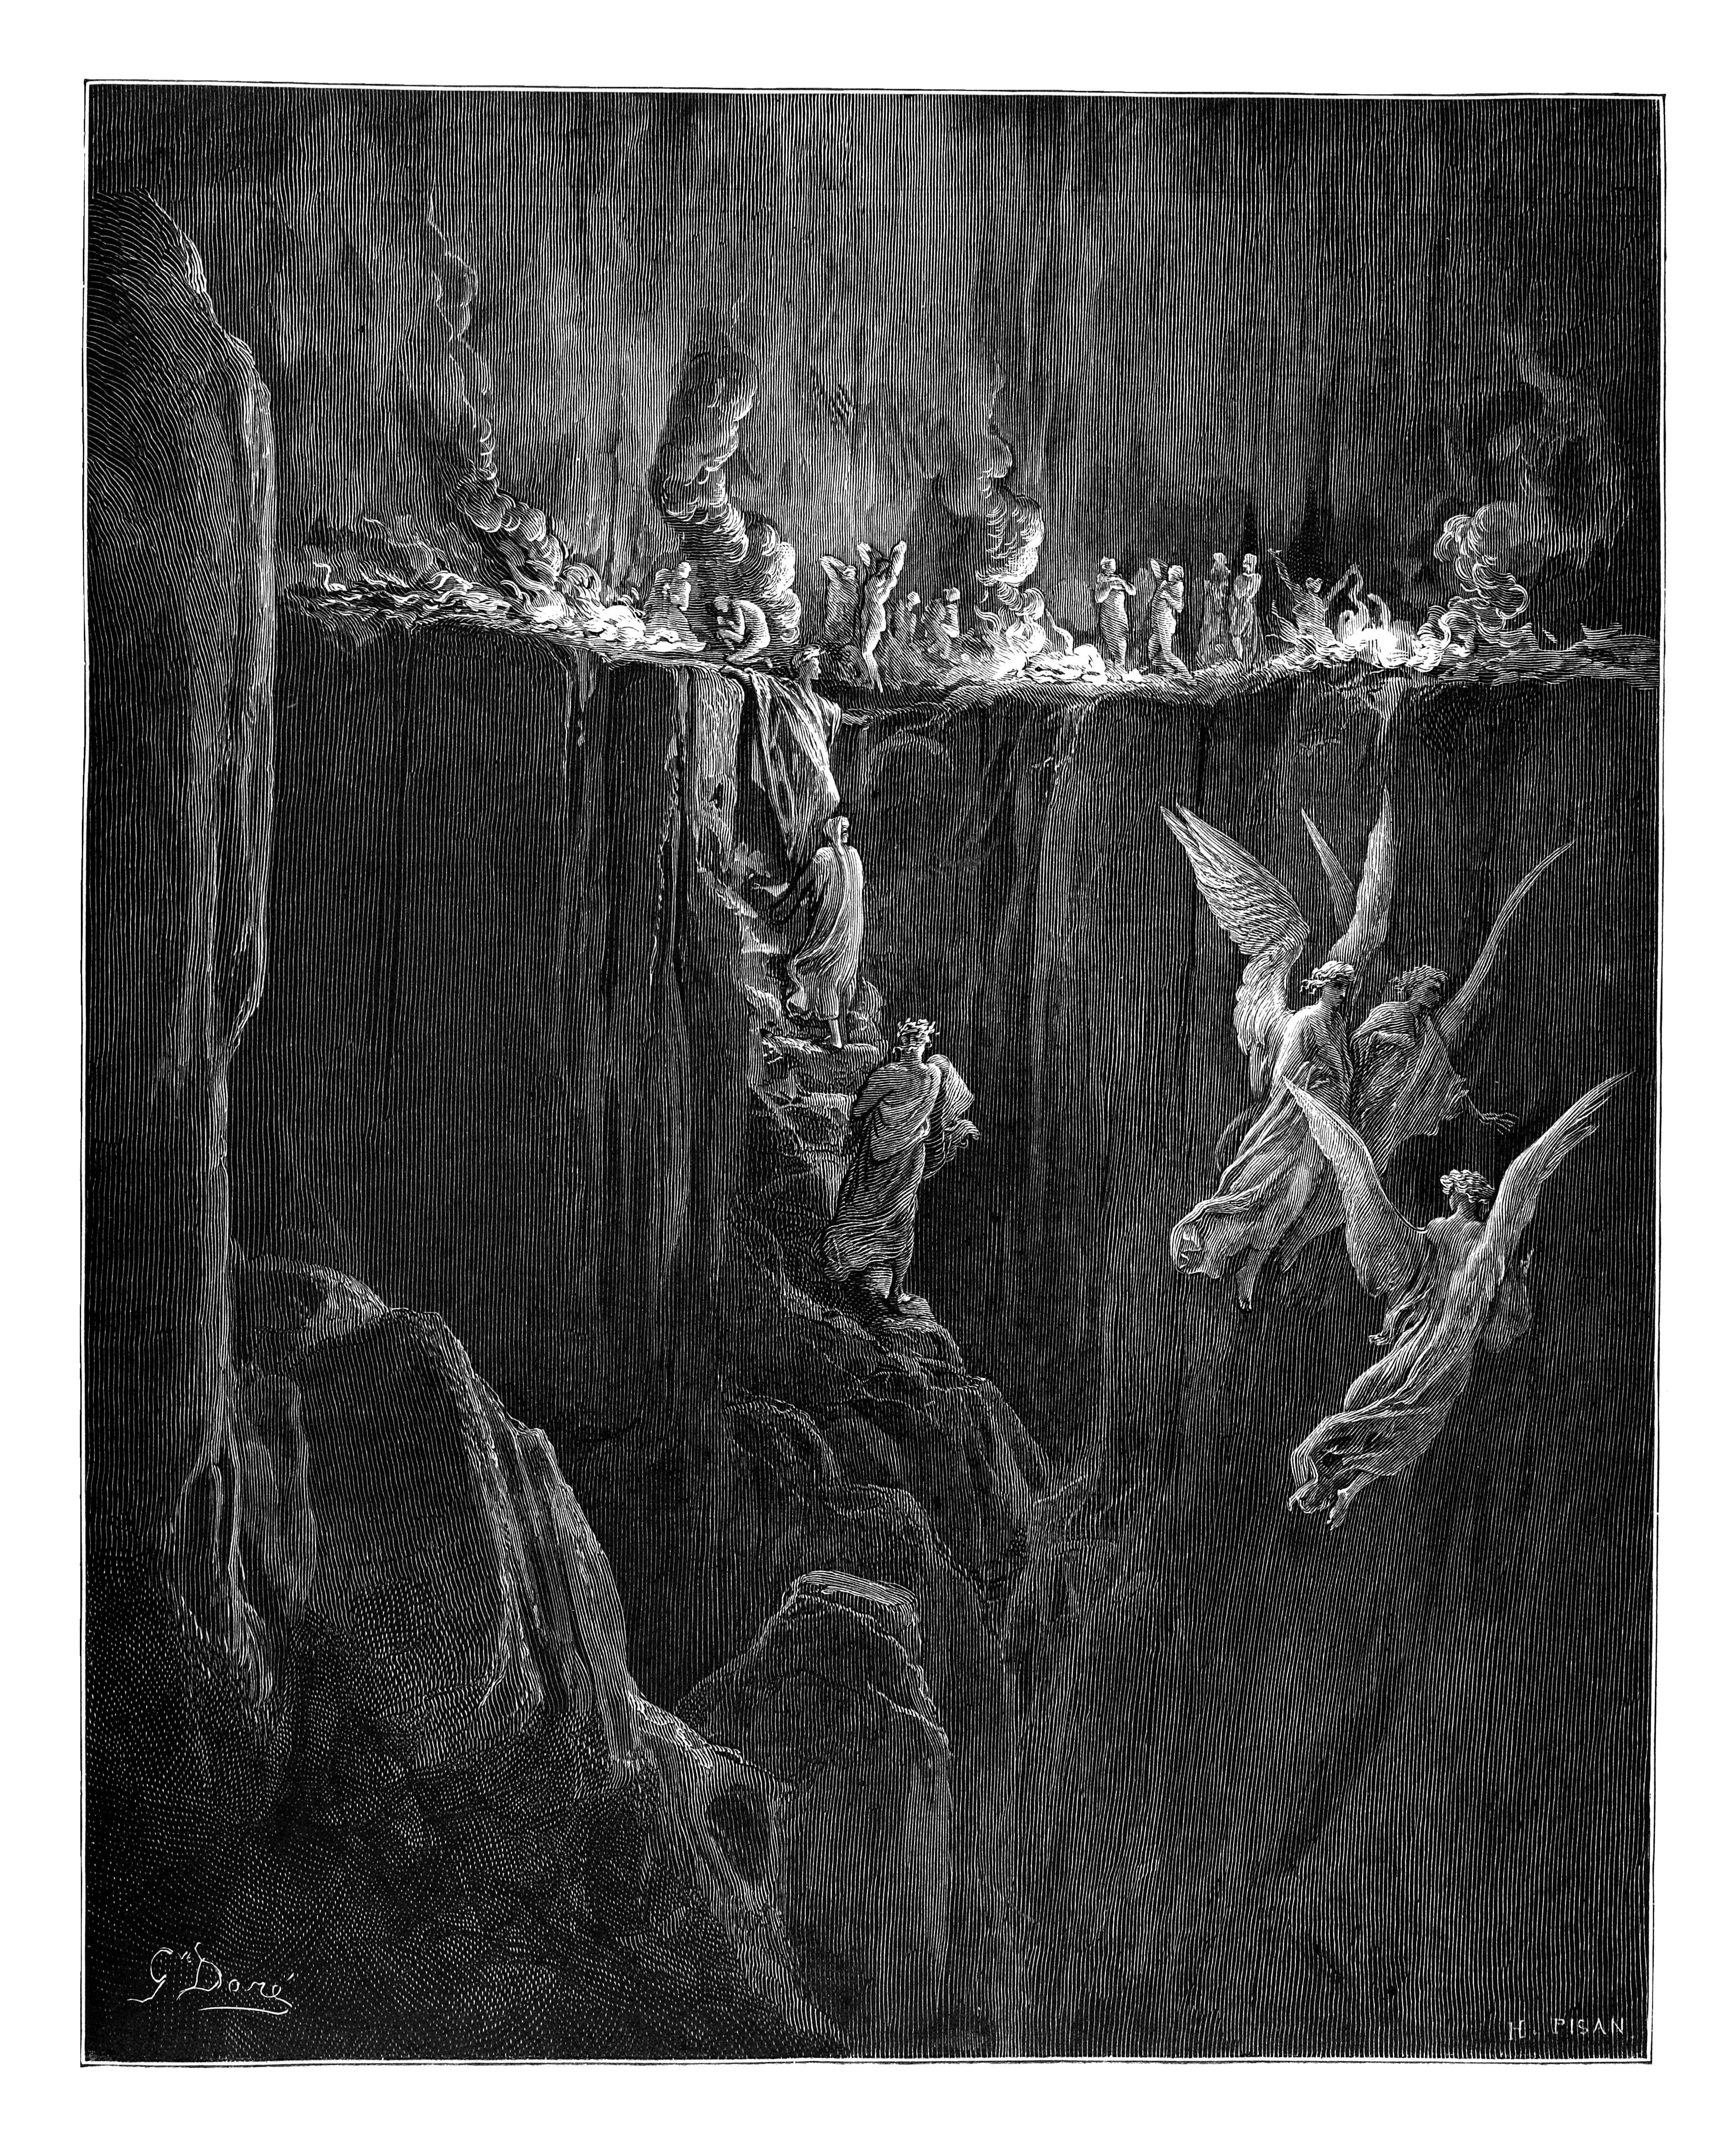
\includegraphics[height=\figsize]{illustrations/book_2/V02, c25.jpg}
\end{figure}

\begin{center}
\begin{minipage}{0.8\linewidth}
\textit{\\
"Lo duca mio dicea: «Per questo loco\\si vuol tenere a li occhi stretto il freno,\\per\`o ch’errar potrebbesi per poco»."} \\
—V02, c25 \\~\\
\textit{"...thus th' instructor warn'd:\\ \textquotesingle Strict rein must in this place direct the eyes.\\A little swerving and the way is lost.\textquotesingle"} \\
—B02, c25
\end{minipage}
\end{center}

\newpage

\section{Canto 26(1)}

\begin{figure}[ht]
\centering
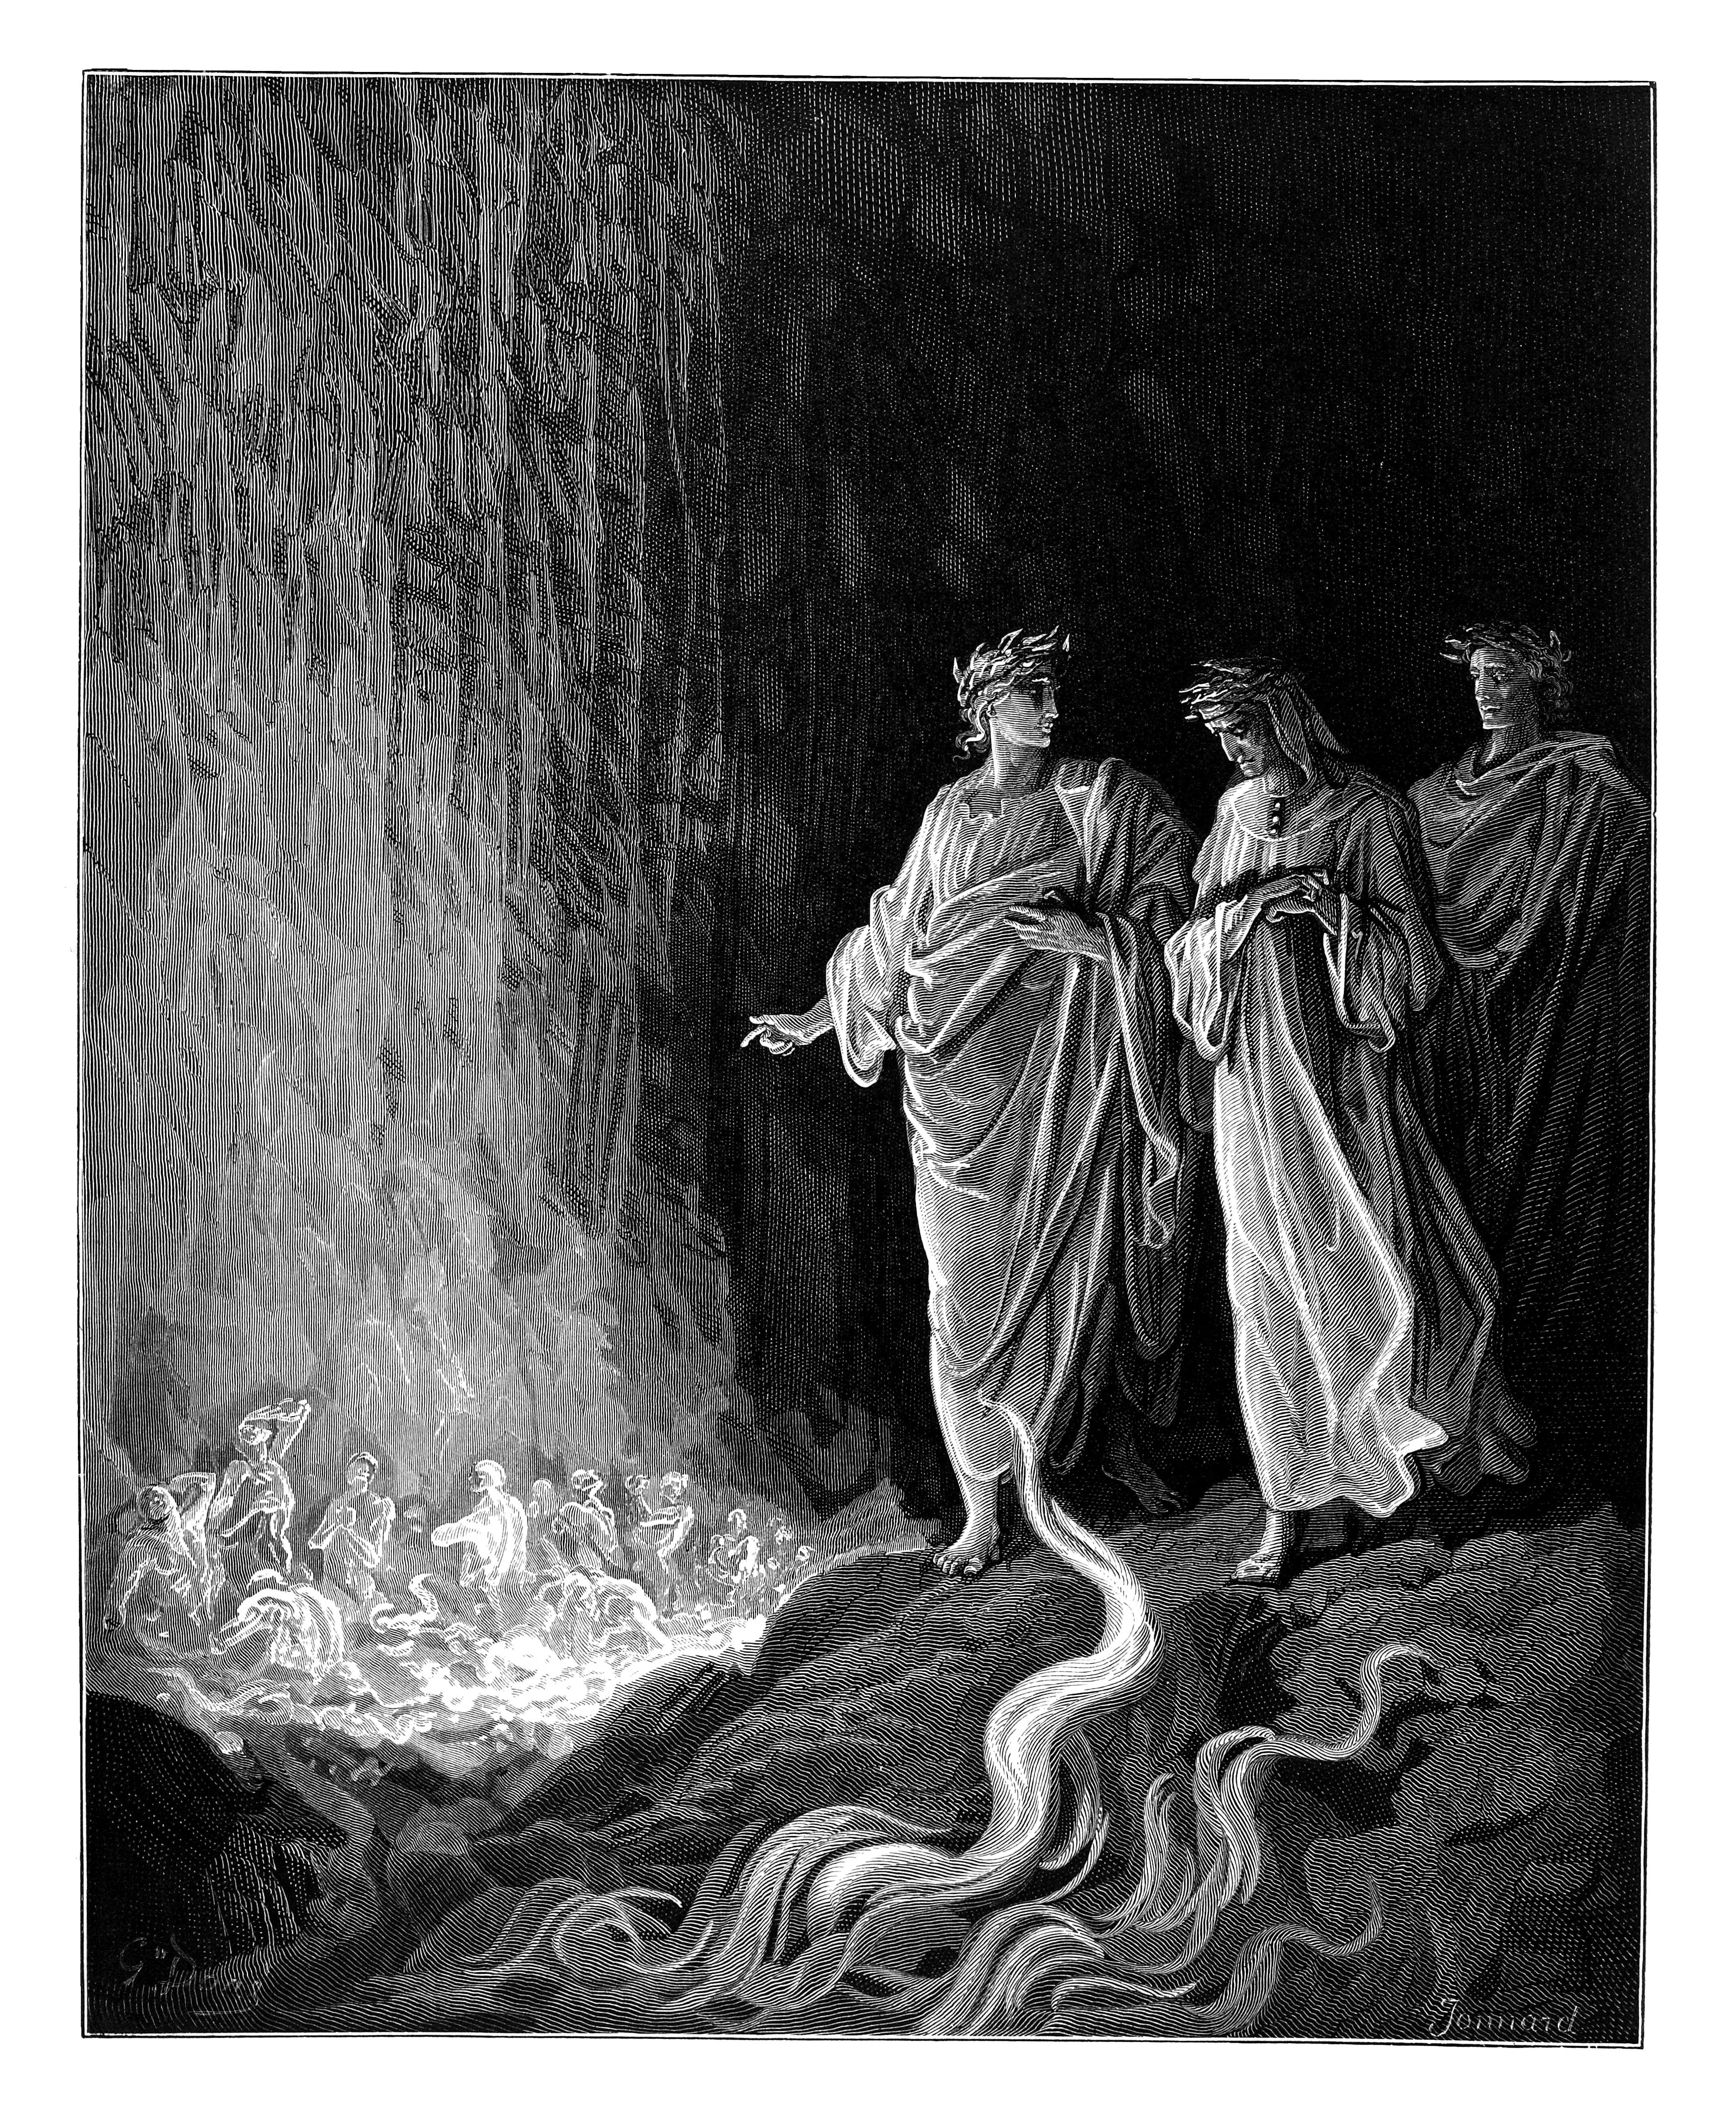
\includegraphics[height=\figsize]{illustrations/book_2/V02, c26(1).jpg}
\end{figure}

\begin{center}
\begin{minipage}{0.8\linewidth}
\textit{\\
"…«Guarda: giovi ch’io ti scaltro»;"} \\
—V02, c26(1) \\~\\
\textit{"...\textquotesingle Look thou well.\\Avail it that I caution thee.\textquotesingle…"} \\
—B02, c26(1)
\end{minipage}
\end{center}

\newpage

\section{Canto 26(2)}

\begin{figure}[ht]
\centering
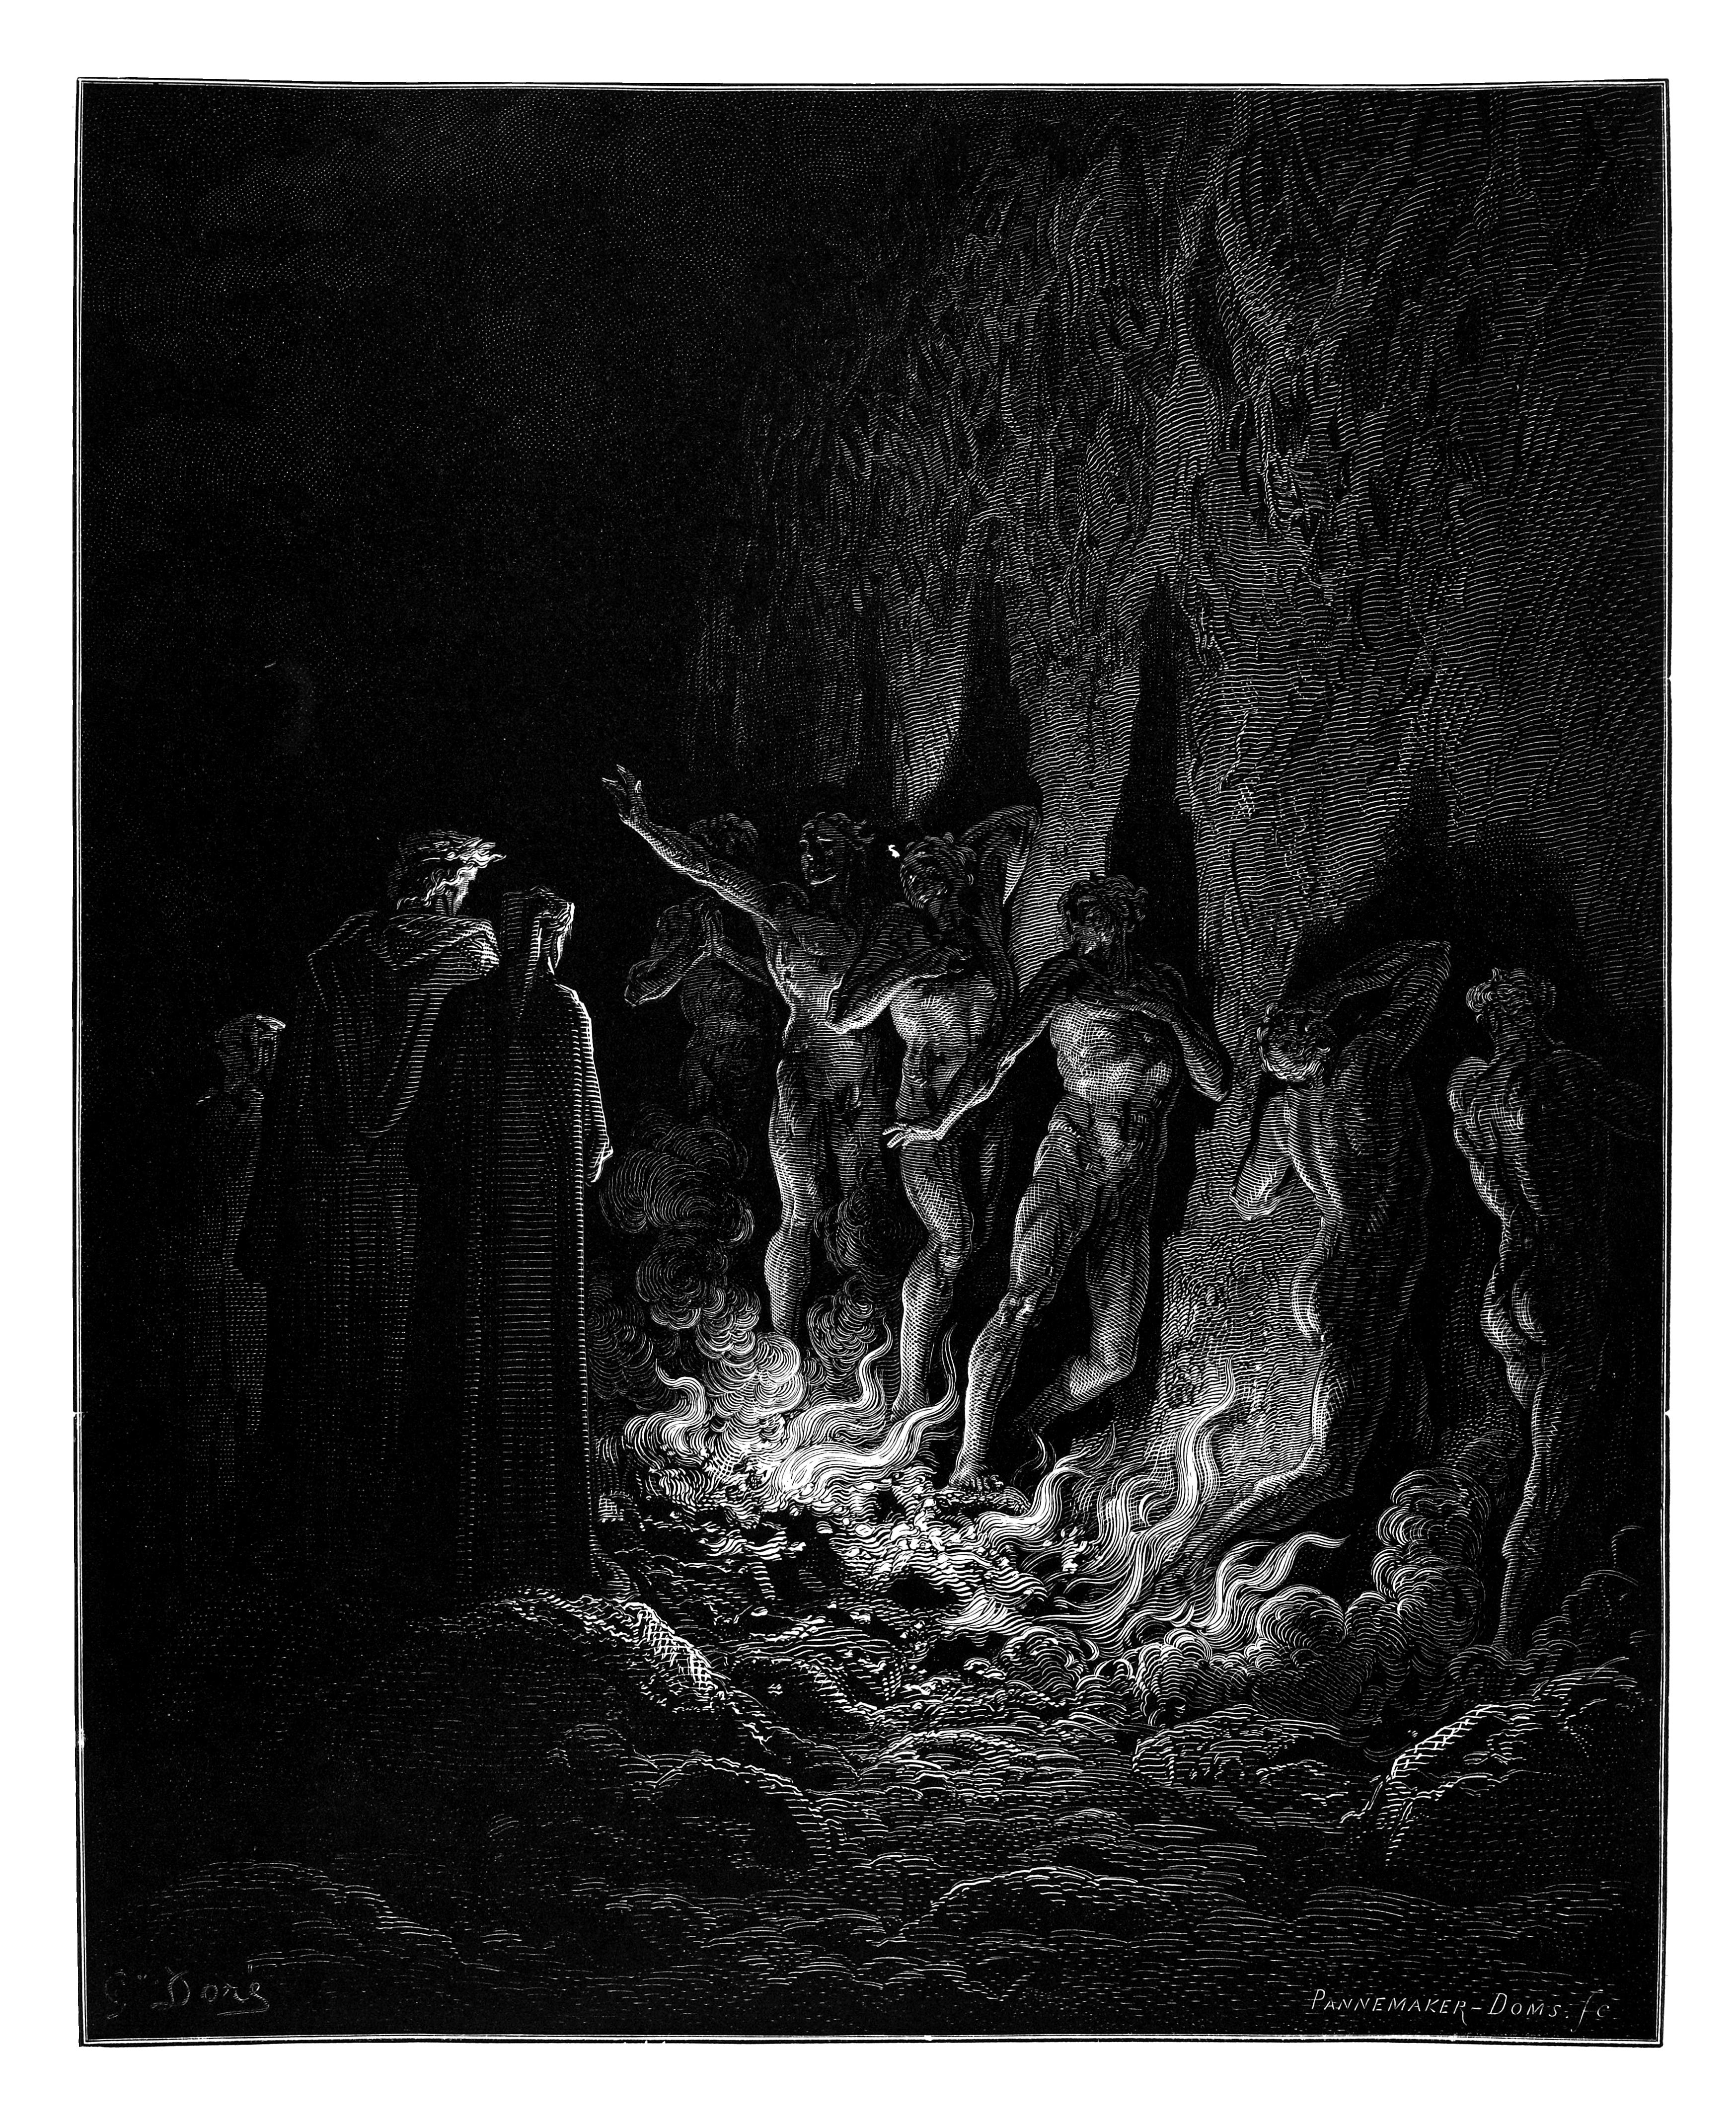
\includegraphics[height=\figsize]{illustrations/book_2/V02, c26(2).jpg}
\end{figure}

\begin{center}
\begin{minipage}{0.8\linewidth}
\textit{\\
"...verso me, quanto potean farsi,\\certi si fero, sempre con riguardo\\di non uscir dove non fosser arsi."} \\
—V02, c26(2) \\~\\
\textit{"...to obtain what certainty they might,\\Stretch'd towards me, careful not to overpass\\The burning pale. …"} \\
—B02, c26(2)
\end{minipage}
\end{center}

\newpage

\section{Canto 27}

\begin{figure}[ht]
\centering
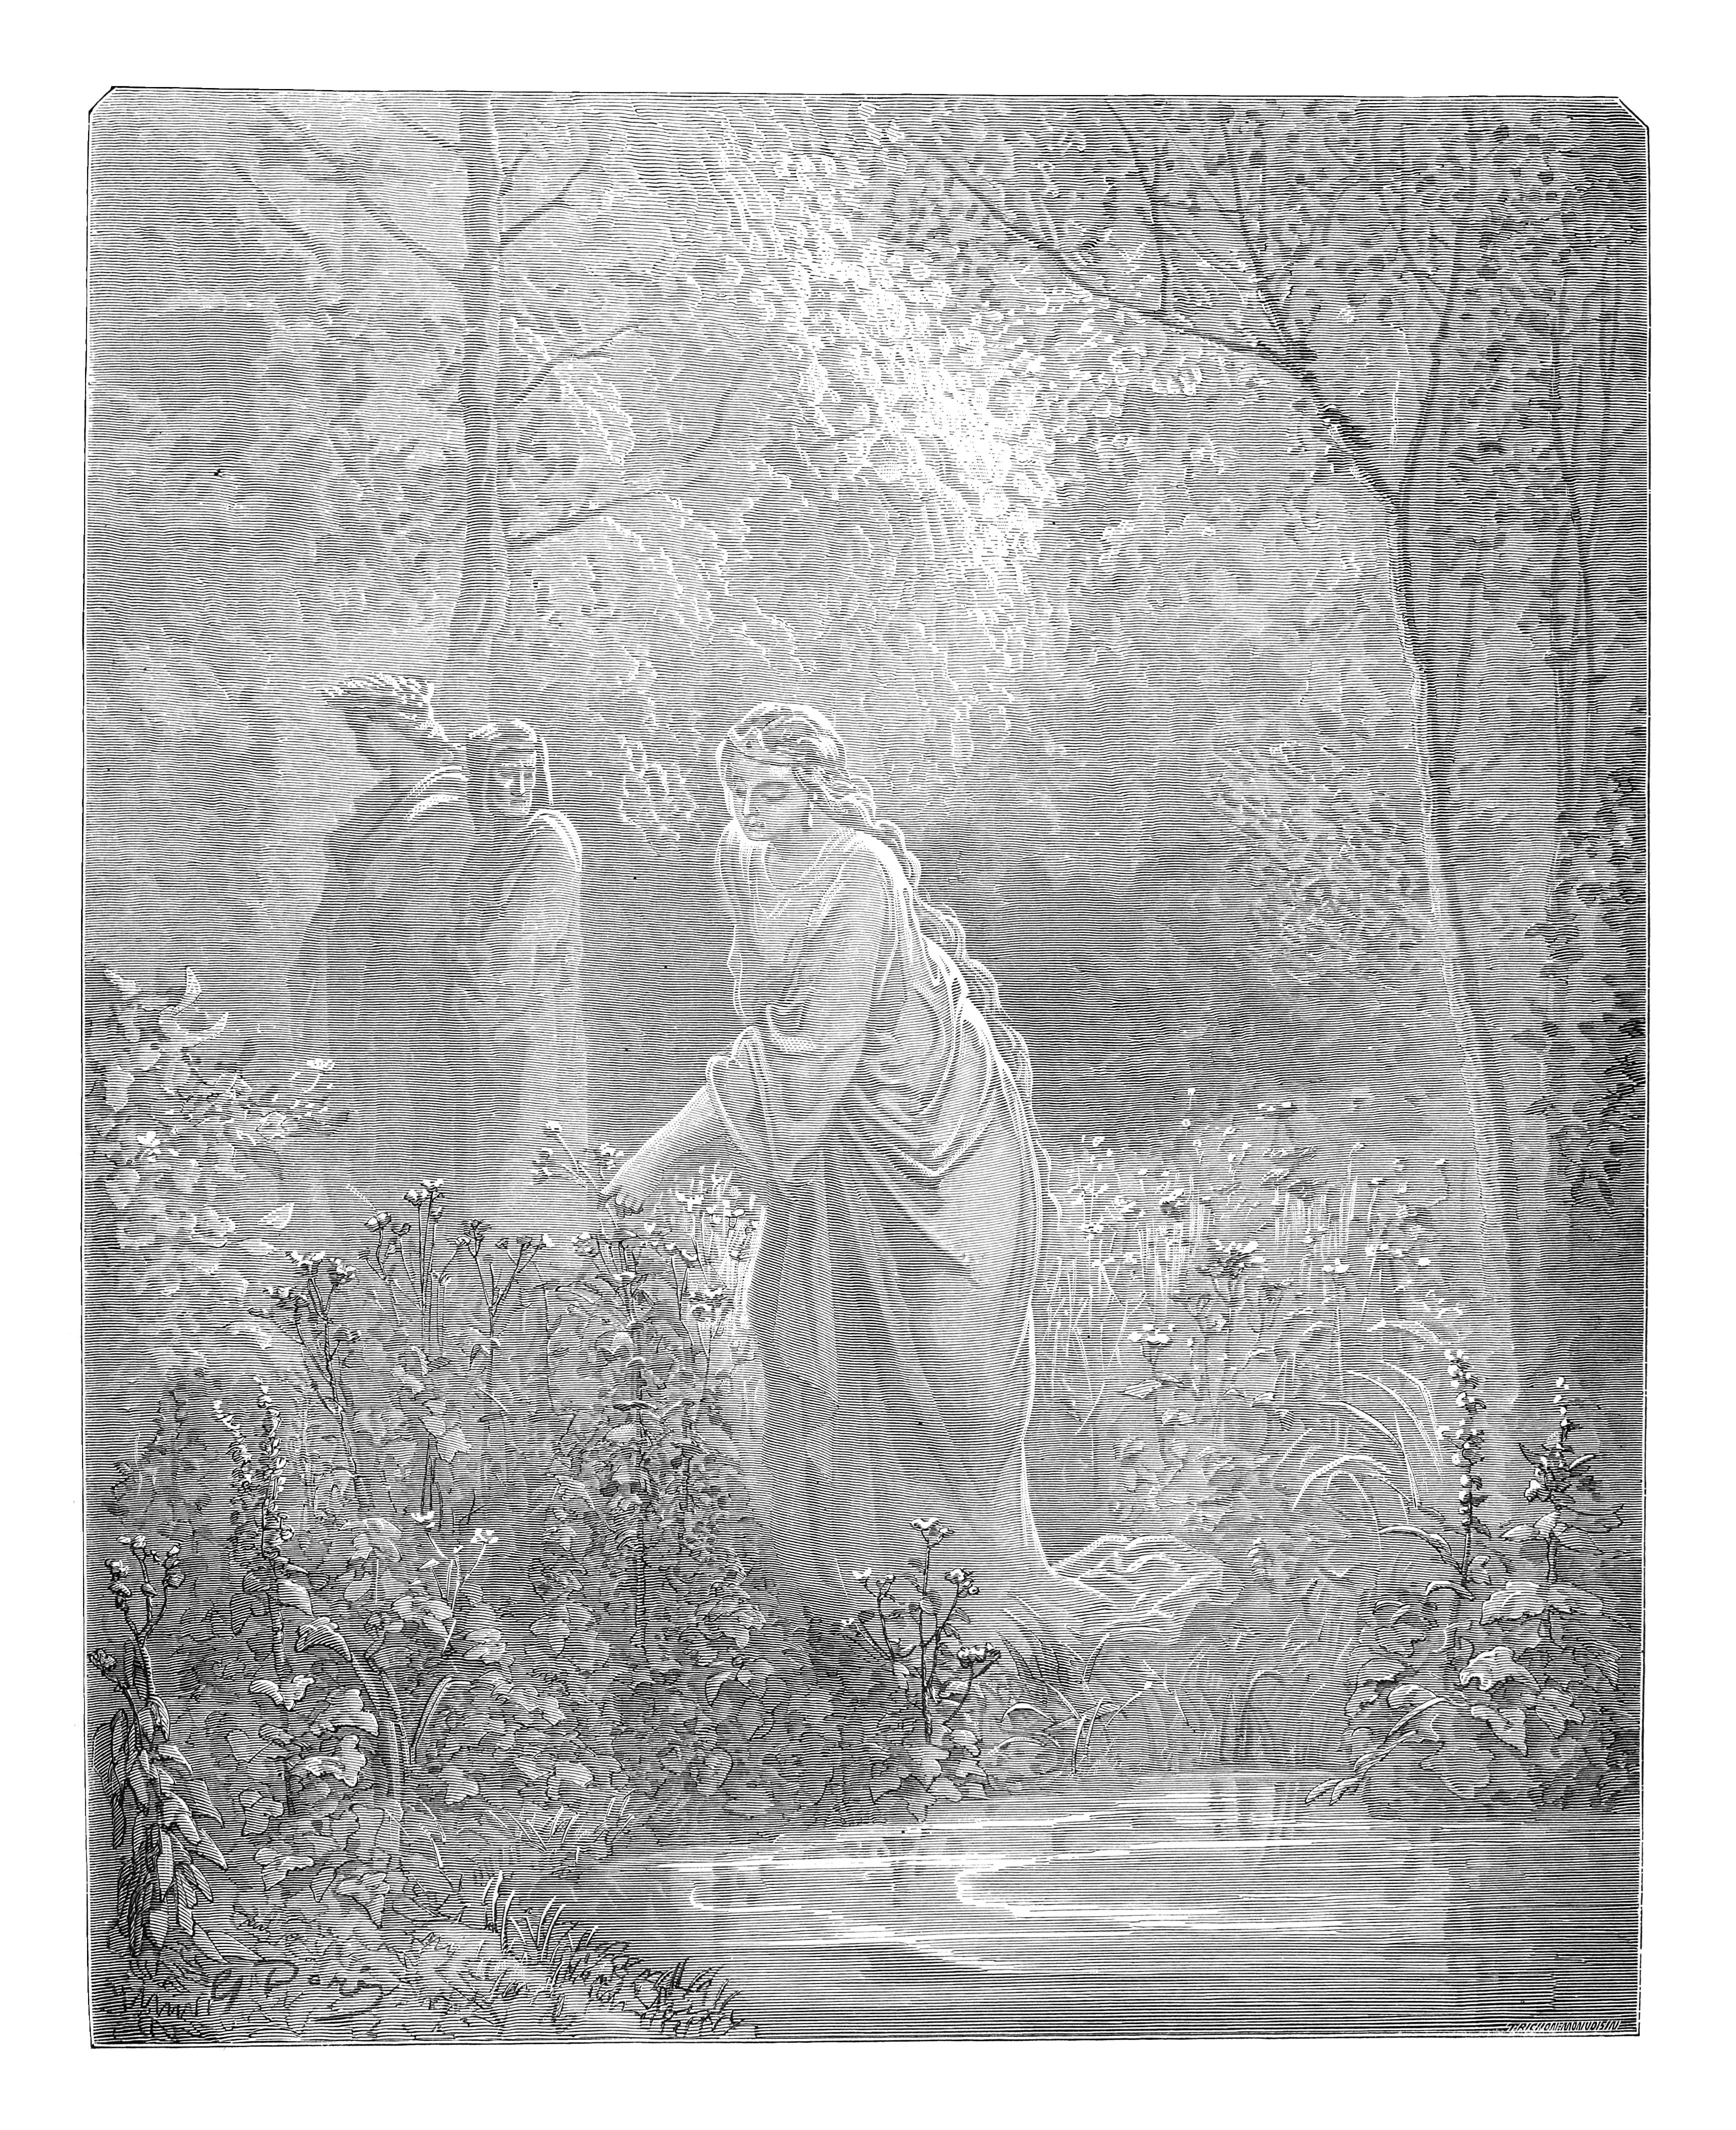
\includegraphics[height=\figsize]{illustrations/book_2/V02, c27.jpg}
\end{figure}

\begin{center}
\begin{minipage}{0.8\linewidth}
\textit{\\
"giovane e bella in sogno mi parea\\donna vedere andar per una landa"} \\
—V02, c27 \\~\\
\textit{"A lady young and beautiful, I dream'd,\\Was passing o'er a lea; …"} \\
—B02, c27
\end{minipage}
\end{center}

\newpage

\section{Canto 28}

\begin{figure}[ht]
\centering
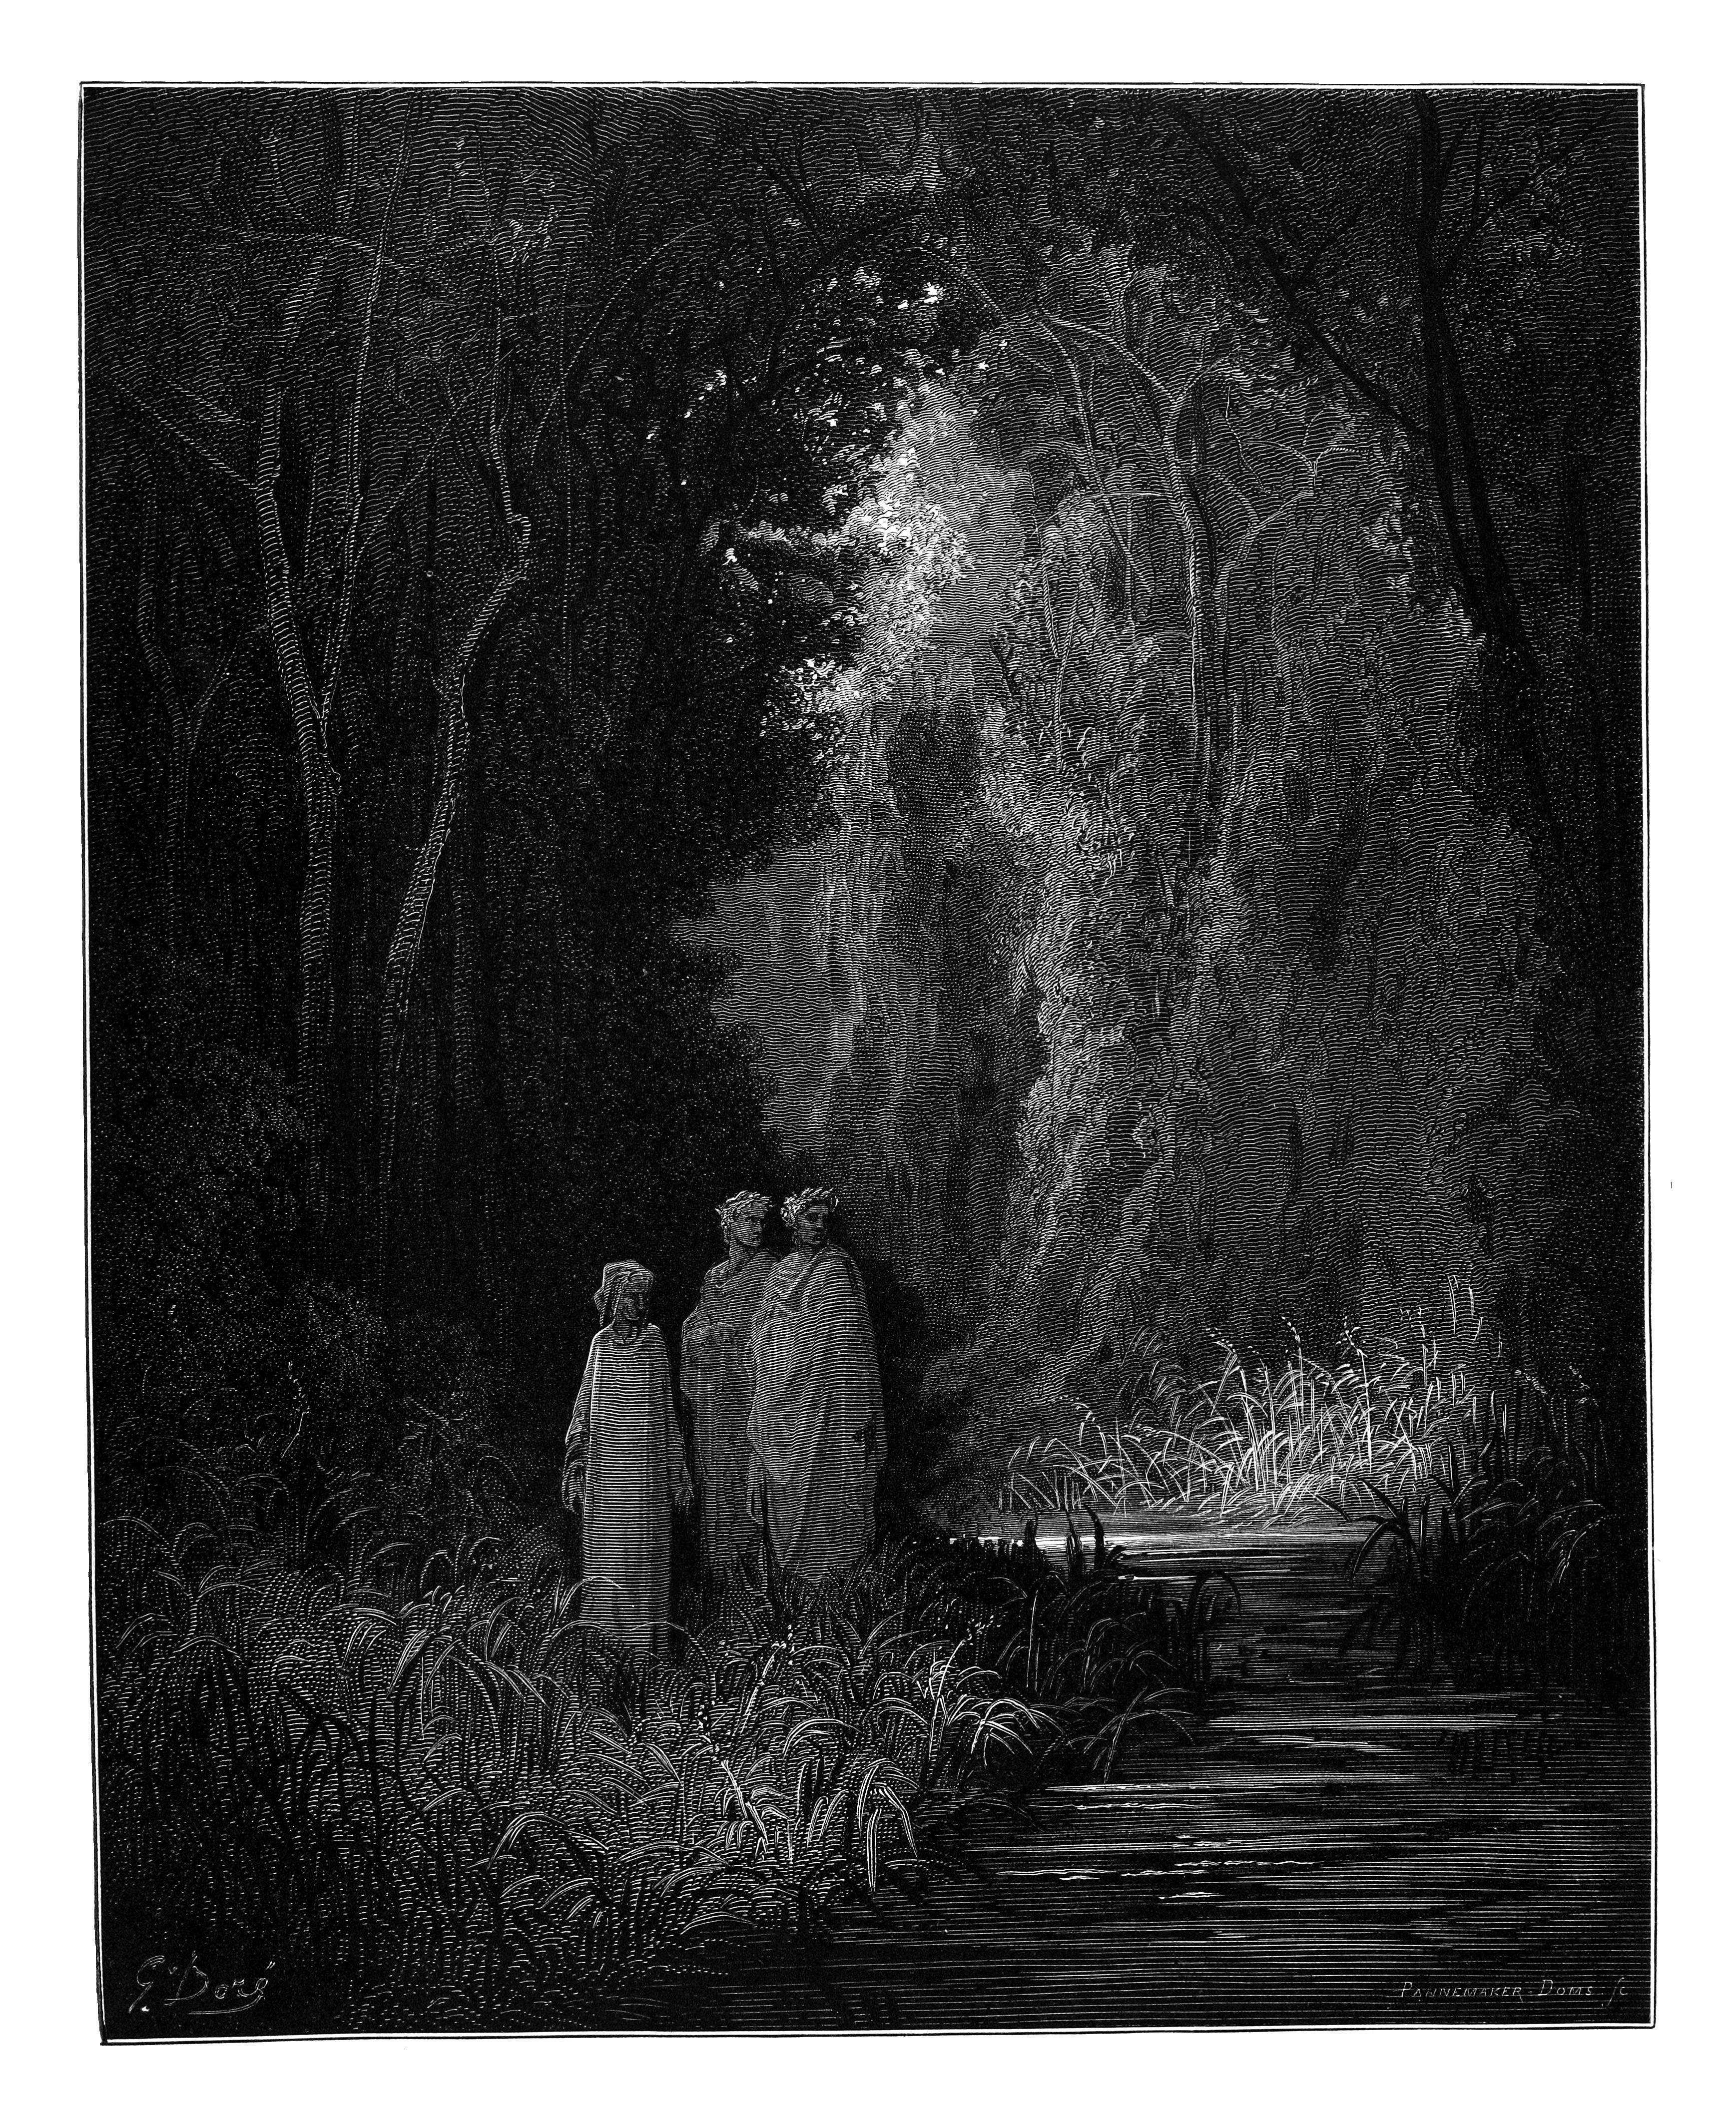
\includegraphics[height=\figsize]{illustrations/book_2/V02, c28.jpg}
\end{figure}

\begin{center}
\begin{minipage}{0.8\linewidth}
\textit{\\
"...ecco più andar mi tolse un rio,\\che ’nver’ sinistra con sue picciole onde\\piegava l’erba che ’n sua ripa usc\`{\i}o."} \\
—V02, c28 \\~\\
\textit{"...behold! my path\\Was bounded by a rill, which to the left\\With little rippling waters bent the grass,\\That issued from its brink. …"} \\
—B02, c28
\end{minipage}
\end{center}

\newpage

\section{Canto 29(1)}

\begin{figure}[ht]
\centering
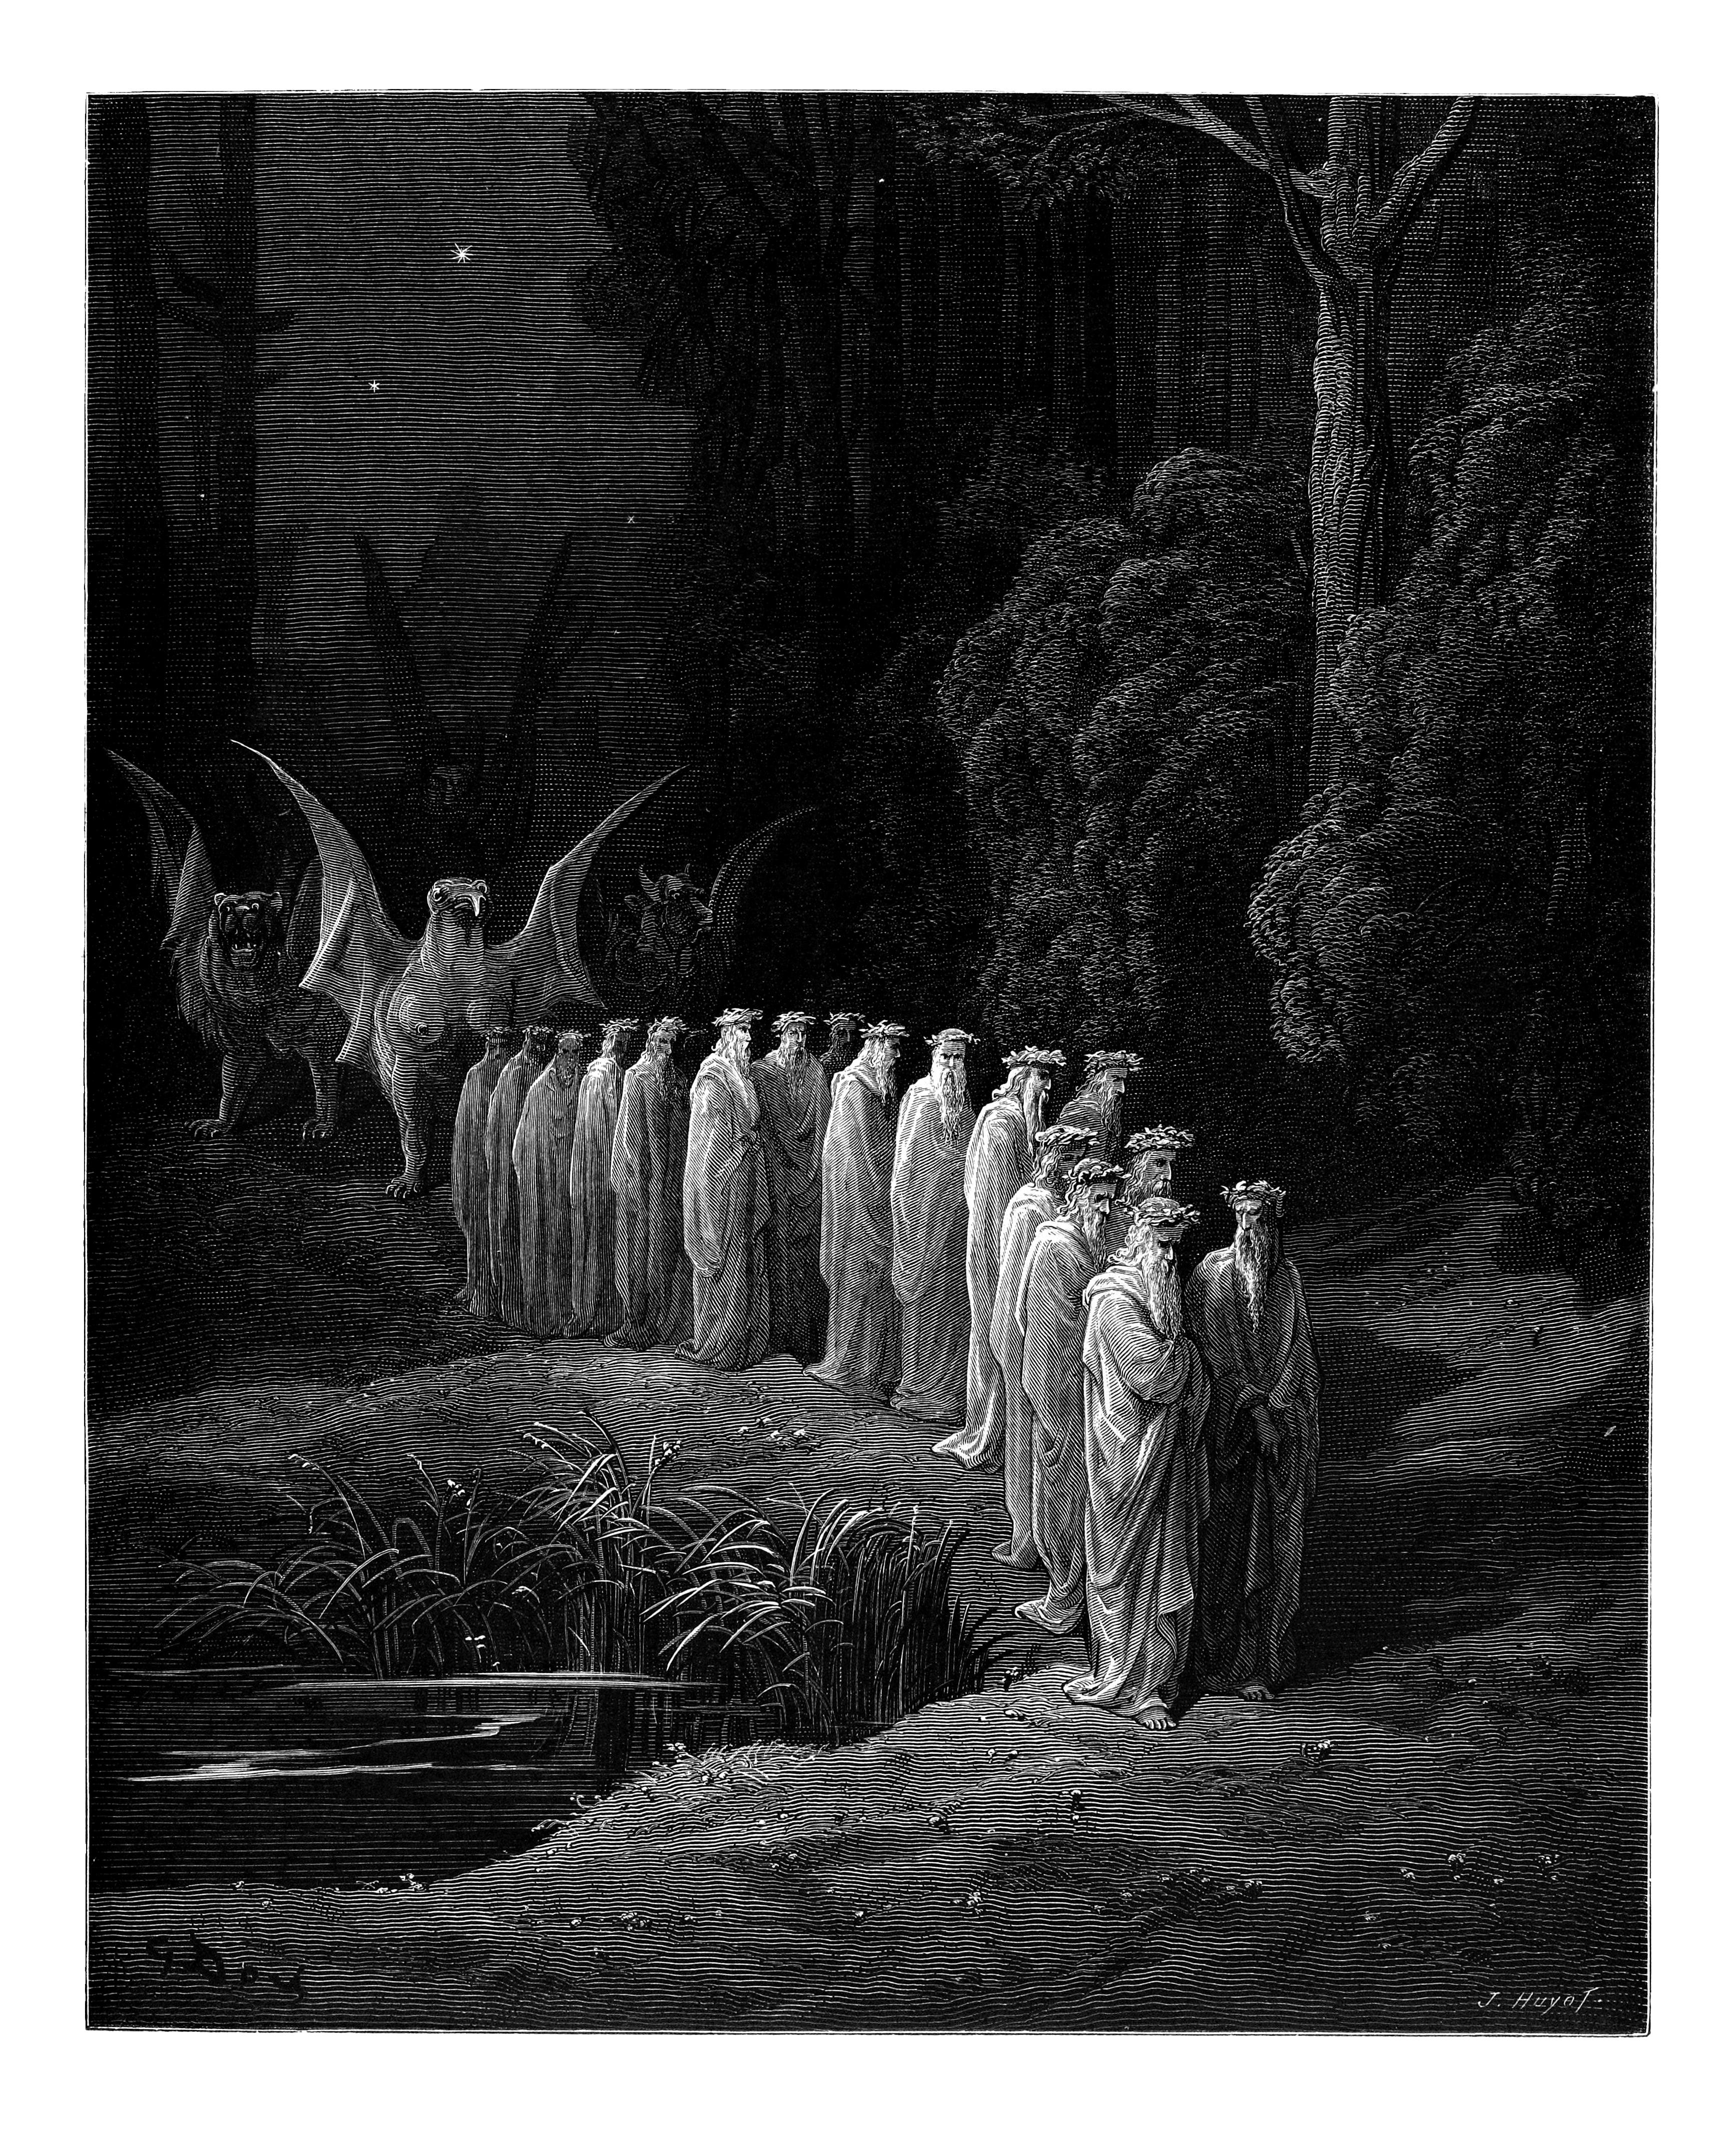
\includegraphics[height=\figsize]{illustrations/book_2/V02, c29(1).jpg}
\end{figure}

\begin{center}
\begin{minipage}{0.8\linewidth}
\textit{\\
"Sotto cos\`{\i} bel ciel com’io diviso,\\ventiquattro seniori, a due a due,\\coronati venien di fiordaliso."} \\
—V02, c29(1) \\~\\
\textit{"...Beneath a sky\\So beautiful, came foul and-twenty elders,\\By two and two, with flower-de-luces crown'd."} \\
—B02, c29(1)
\end{minipage}
\end{center}

\newpage

\section{Canto 29(2)}

\begin{figure}[ht]
\centering
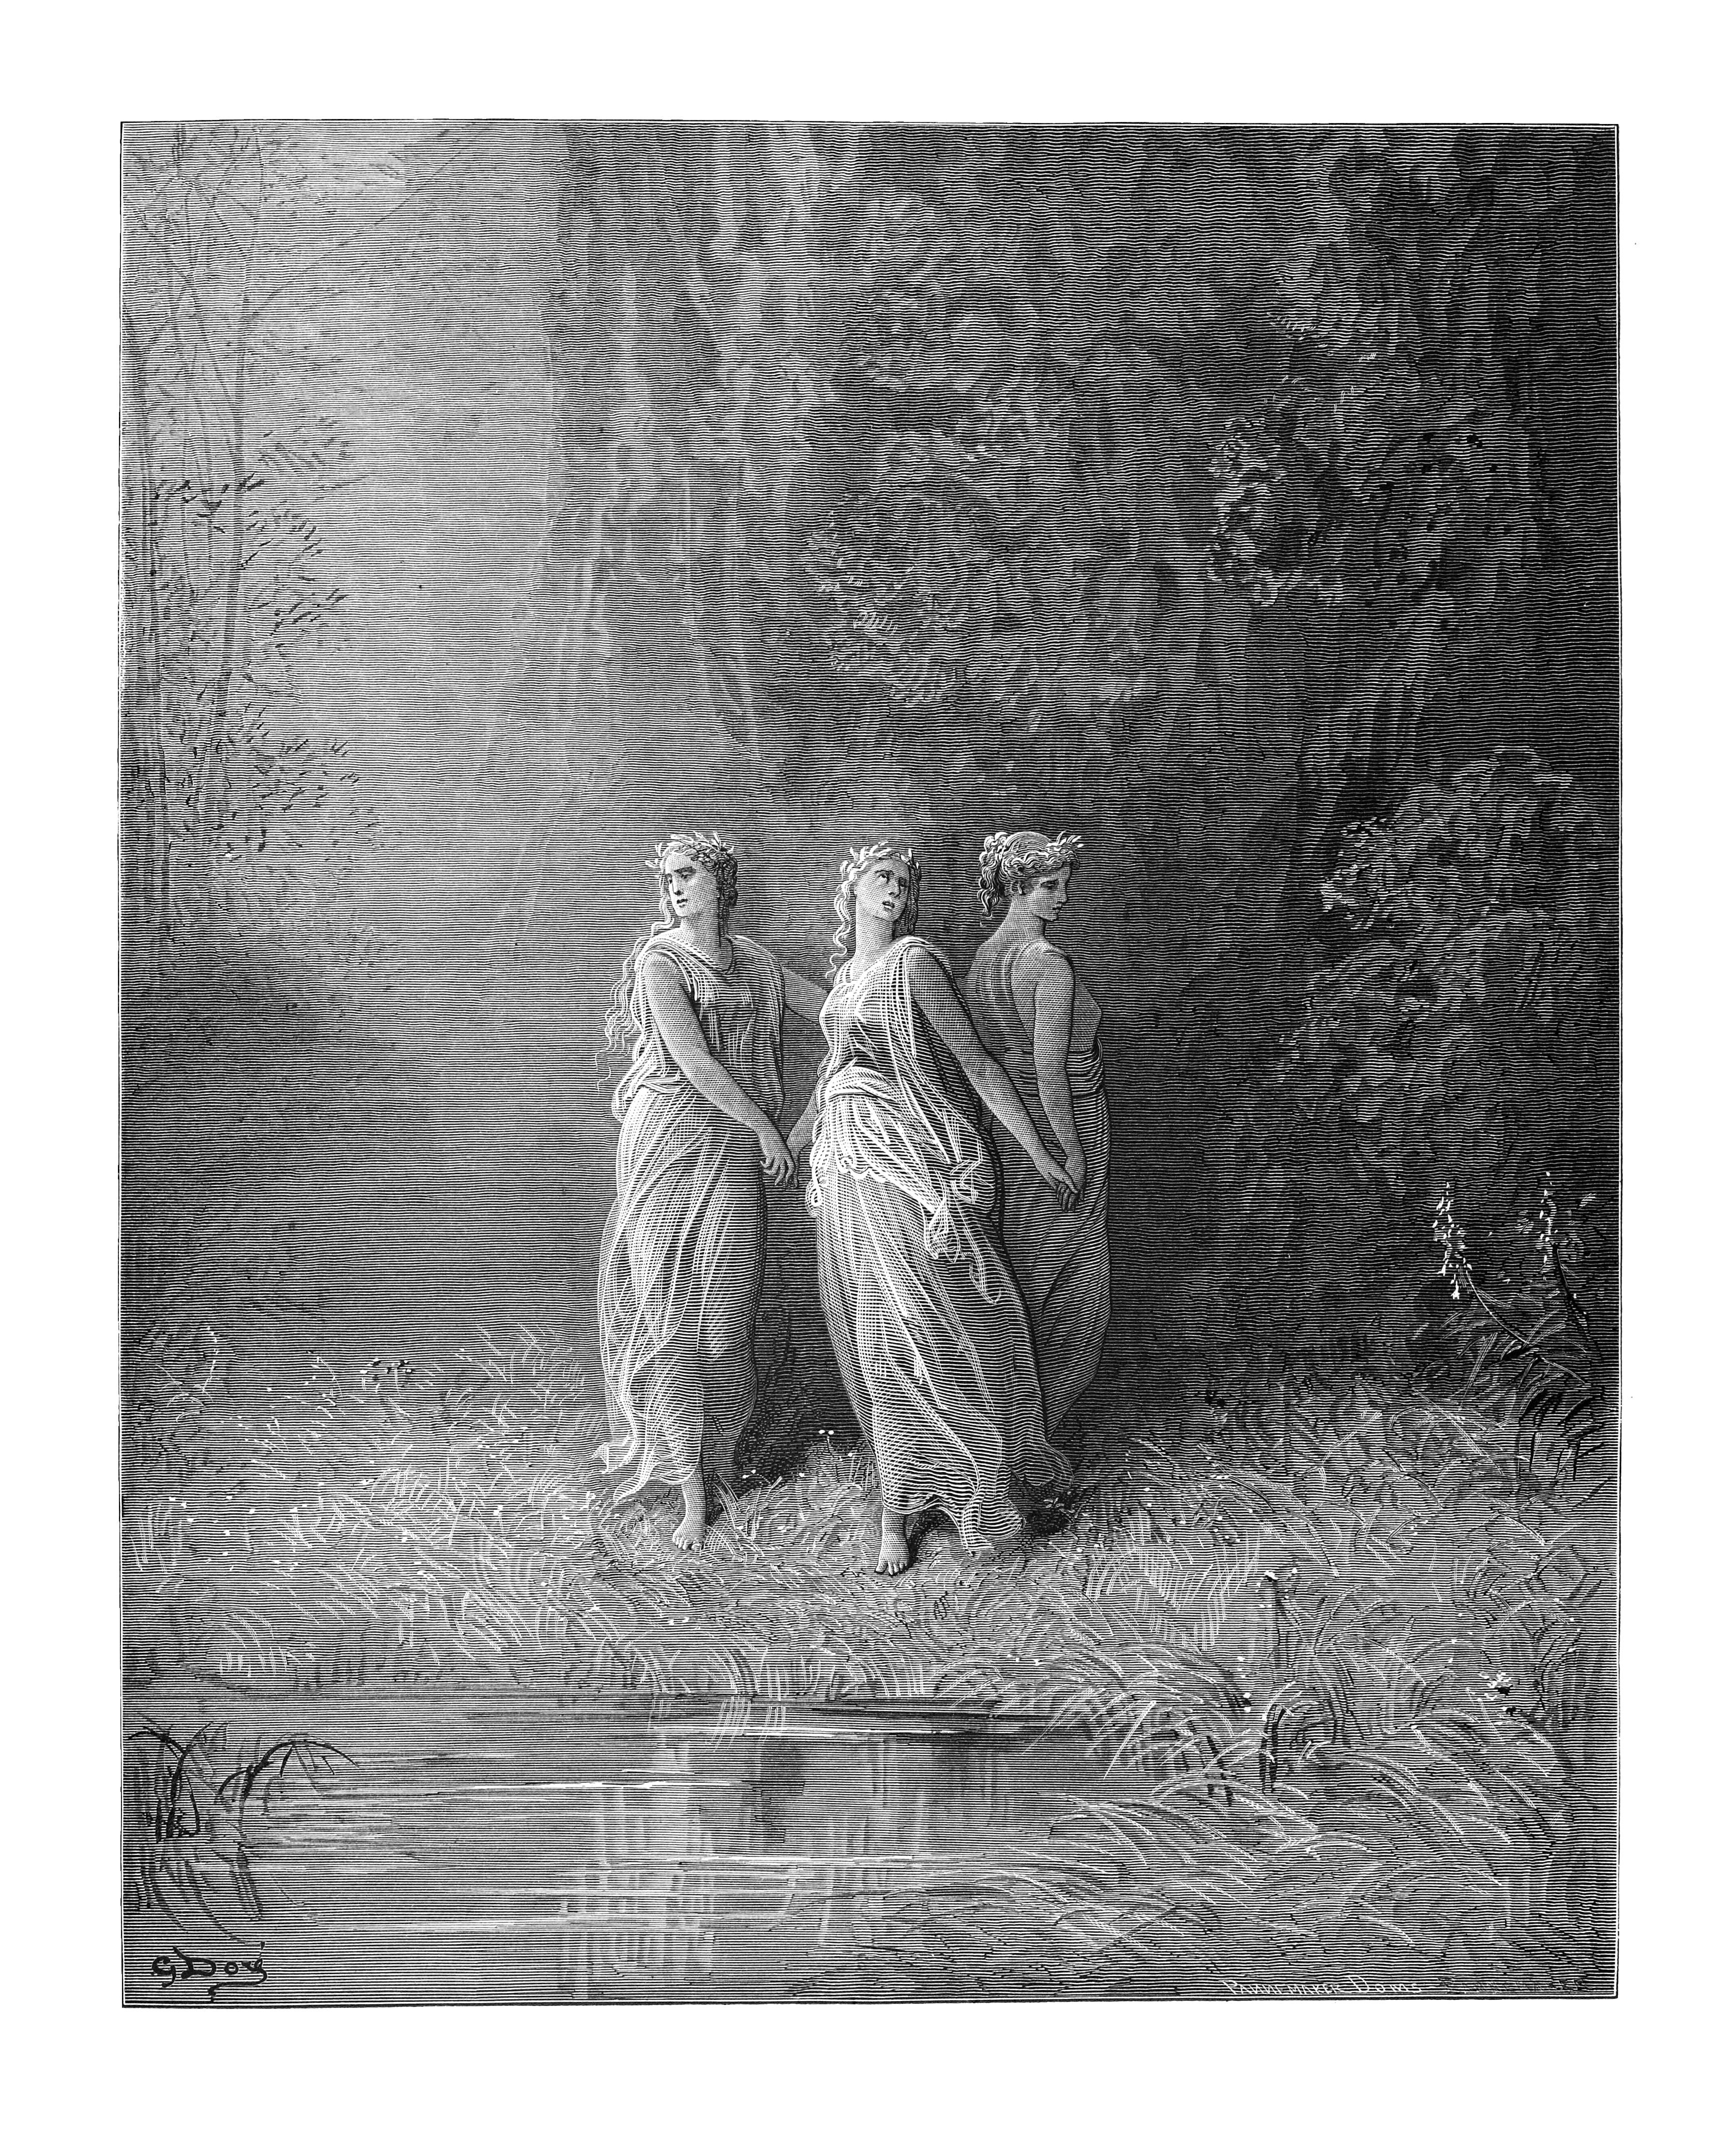
\includegraphics[height=\figsize]{illustrations/book_2/V02, c29(2).jpg}
\end{figure}

\begin{center}
\begin{minipage}{0.8\linewidth}
\textit{\\
"Tre donne in giro da la destra rota\\venian danzando; …"} \\
—V02, c29(2) \\~\\
\textit{"...Three nymphs\\at the right wheel, came circling in smooth dance;"} \\
—B02, c29(2)
\end{minipage}
\end{center}

\newpage

\section{Canto 30}

\begin{figure}[ht]
\centering
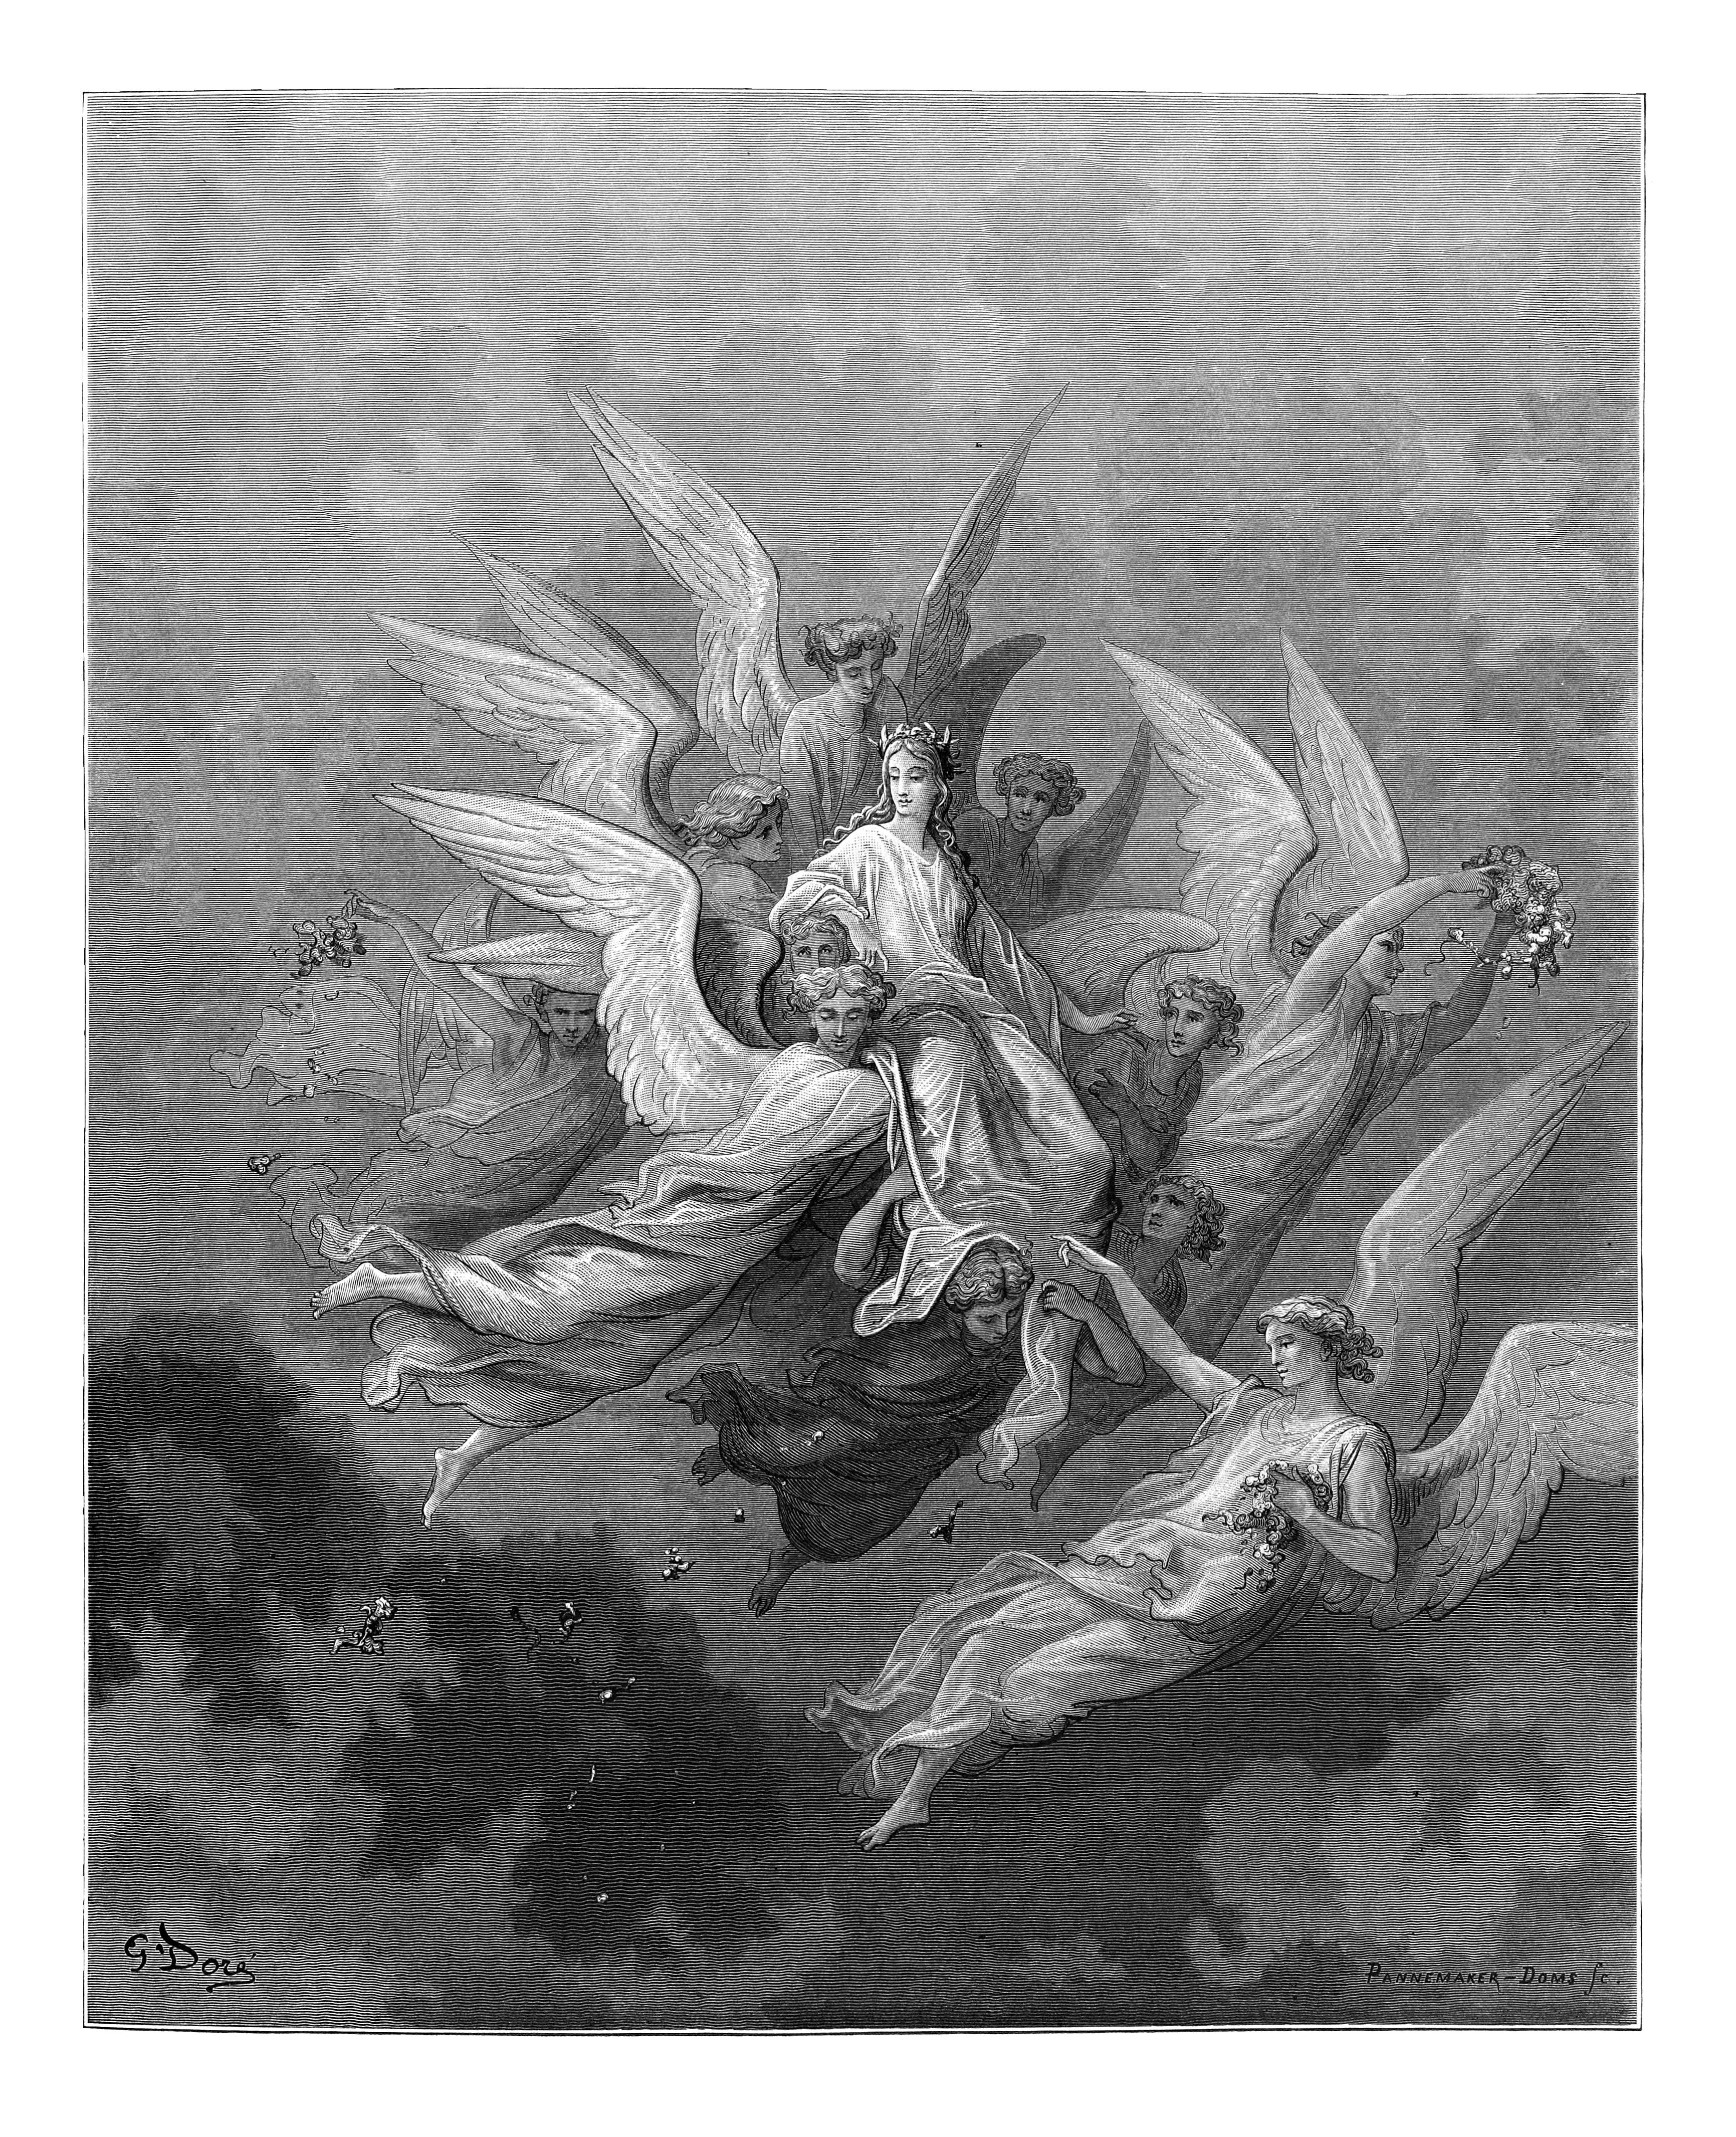
\includegraphics[height=\figsize]{illustrations/book_2/V02, c30.jpg}
\end{figure}

\begin{center}
\begin{minipage}{0.8\linewidth}
\textit{\\
"vidi la donna che pria m’appario\\velata sotto l’angelica festa,\\drizzar li occhi ver’ me di qua dal rio."} \\
—V02, c30 \\~\\
\textit{"Towards me, across the stream, she bent her eyes;"} \\
—B02, c30
\end{minipage}
\end{center}

\newpage

\section{Canto 31}

\begin{figure}[ht]
\centering
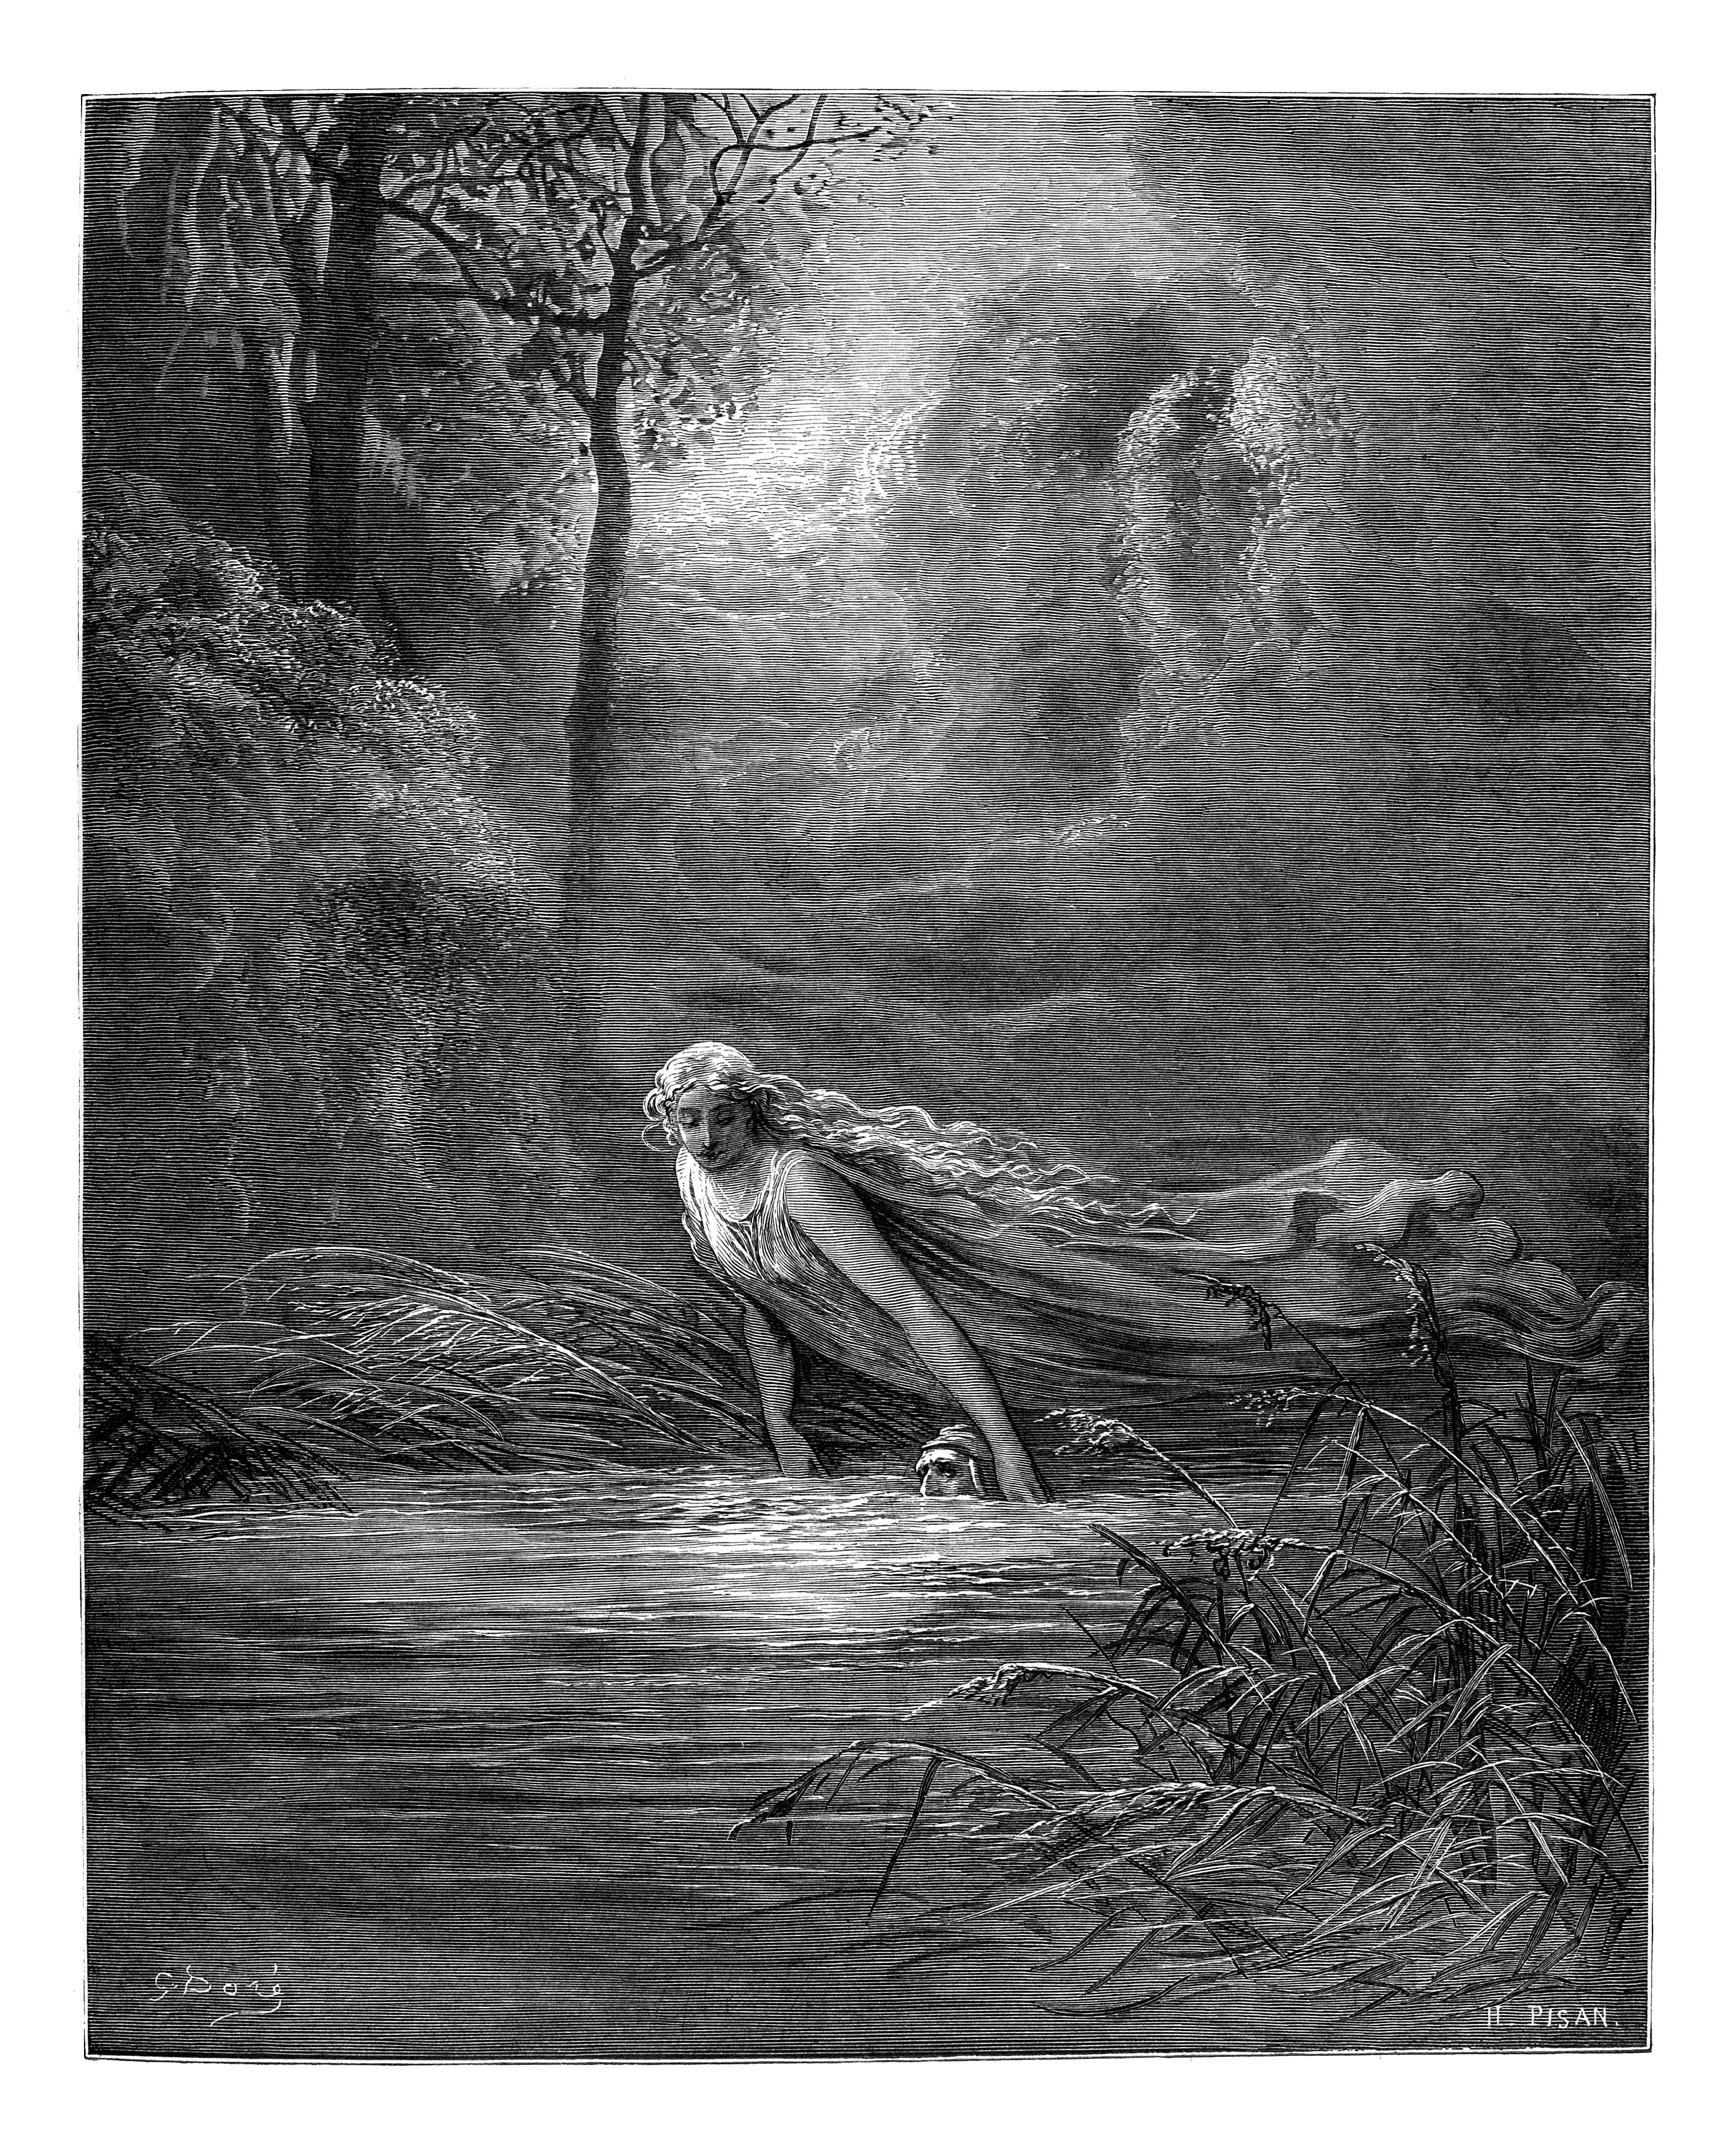
\includegraphics[height=\figsize]{illustrations/book_2/V02, c31.jpg}
\end{figure}

\begin{center}
\begin{minipage}{0.8\linewidth}
\textit{\\
"La bella donna ne le braccia aprissi;\\abbracciommi la testa e mi sommerse\\ove convenne ch’io l’acqua inghiottissi."} \\
—V02, c31 \\~\\
\textit{"The beauteous dame, her arms expanding, clasp'd\\My temples, and immerg'd me, where 't was fit\\The wave should drench me: …"} \\
—B02, c31
\end{minipage}
\end{center}

\newpage

\section{Canto 32}

\begin{figure}[ht]
\centering
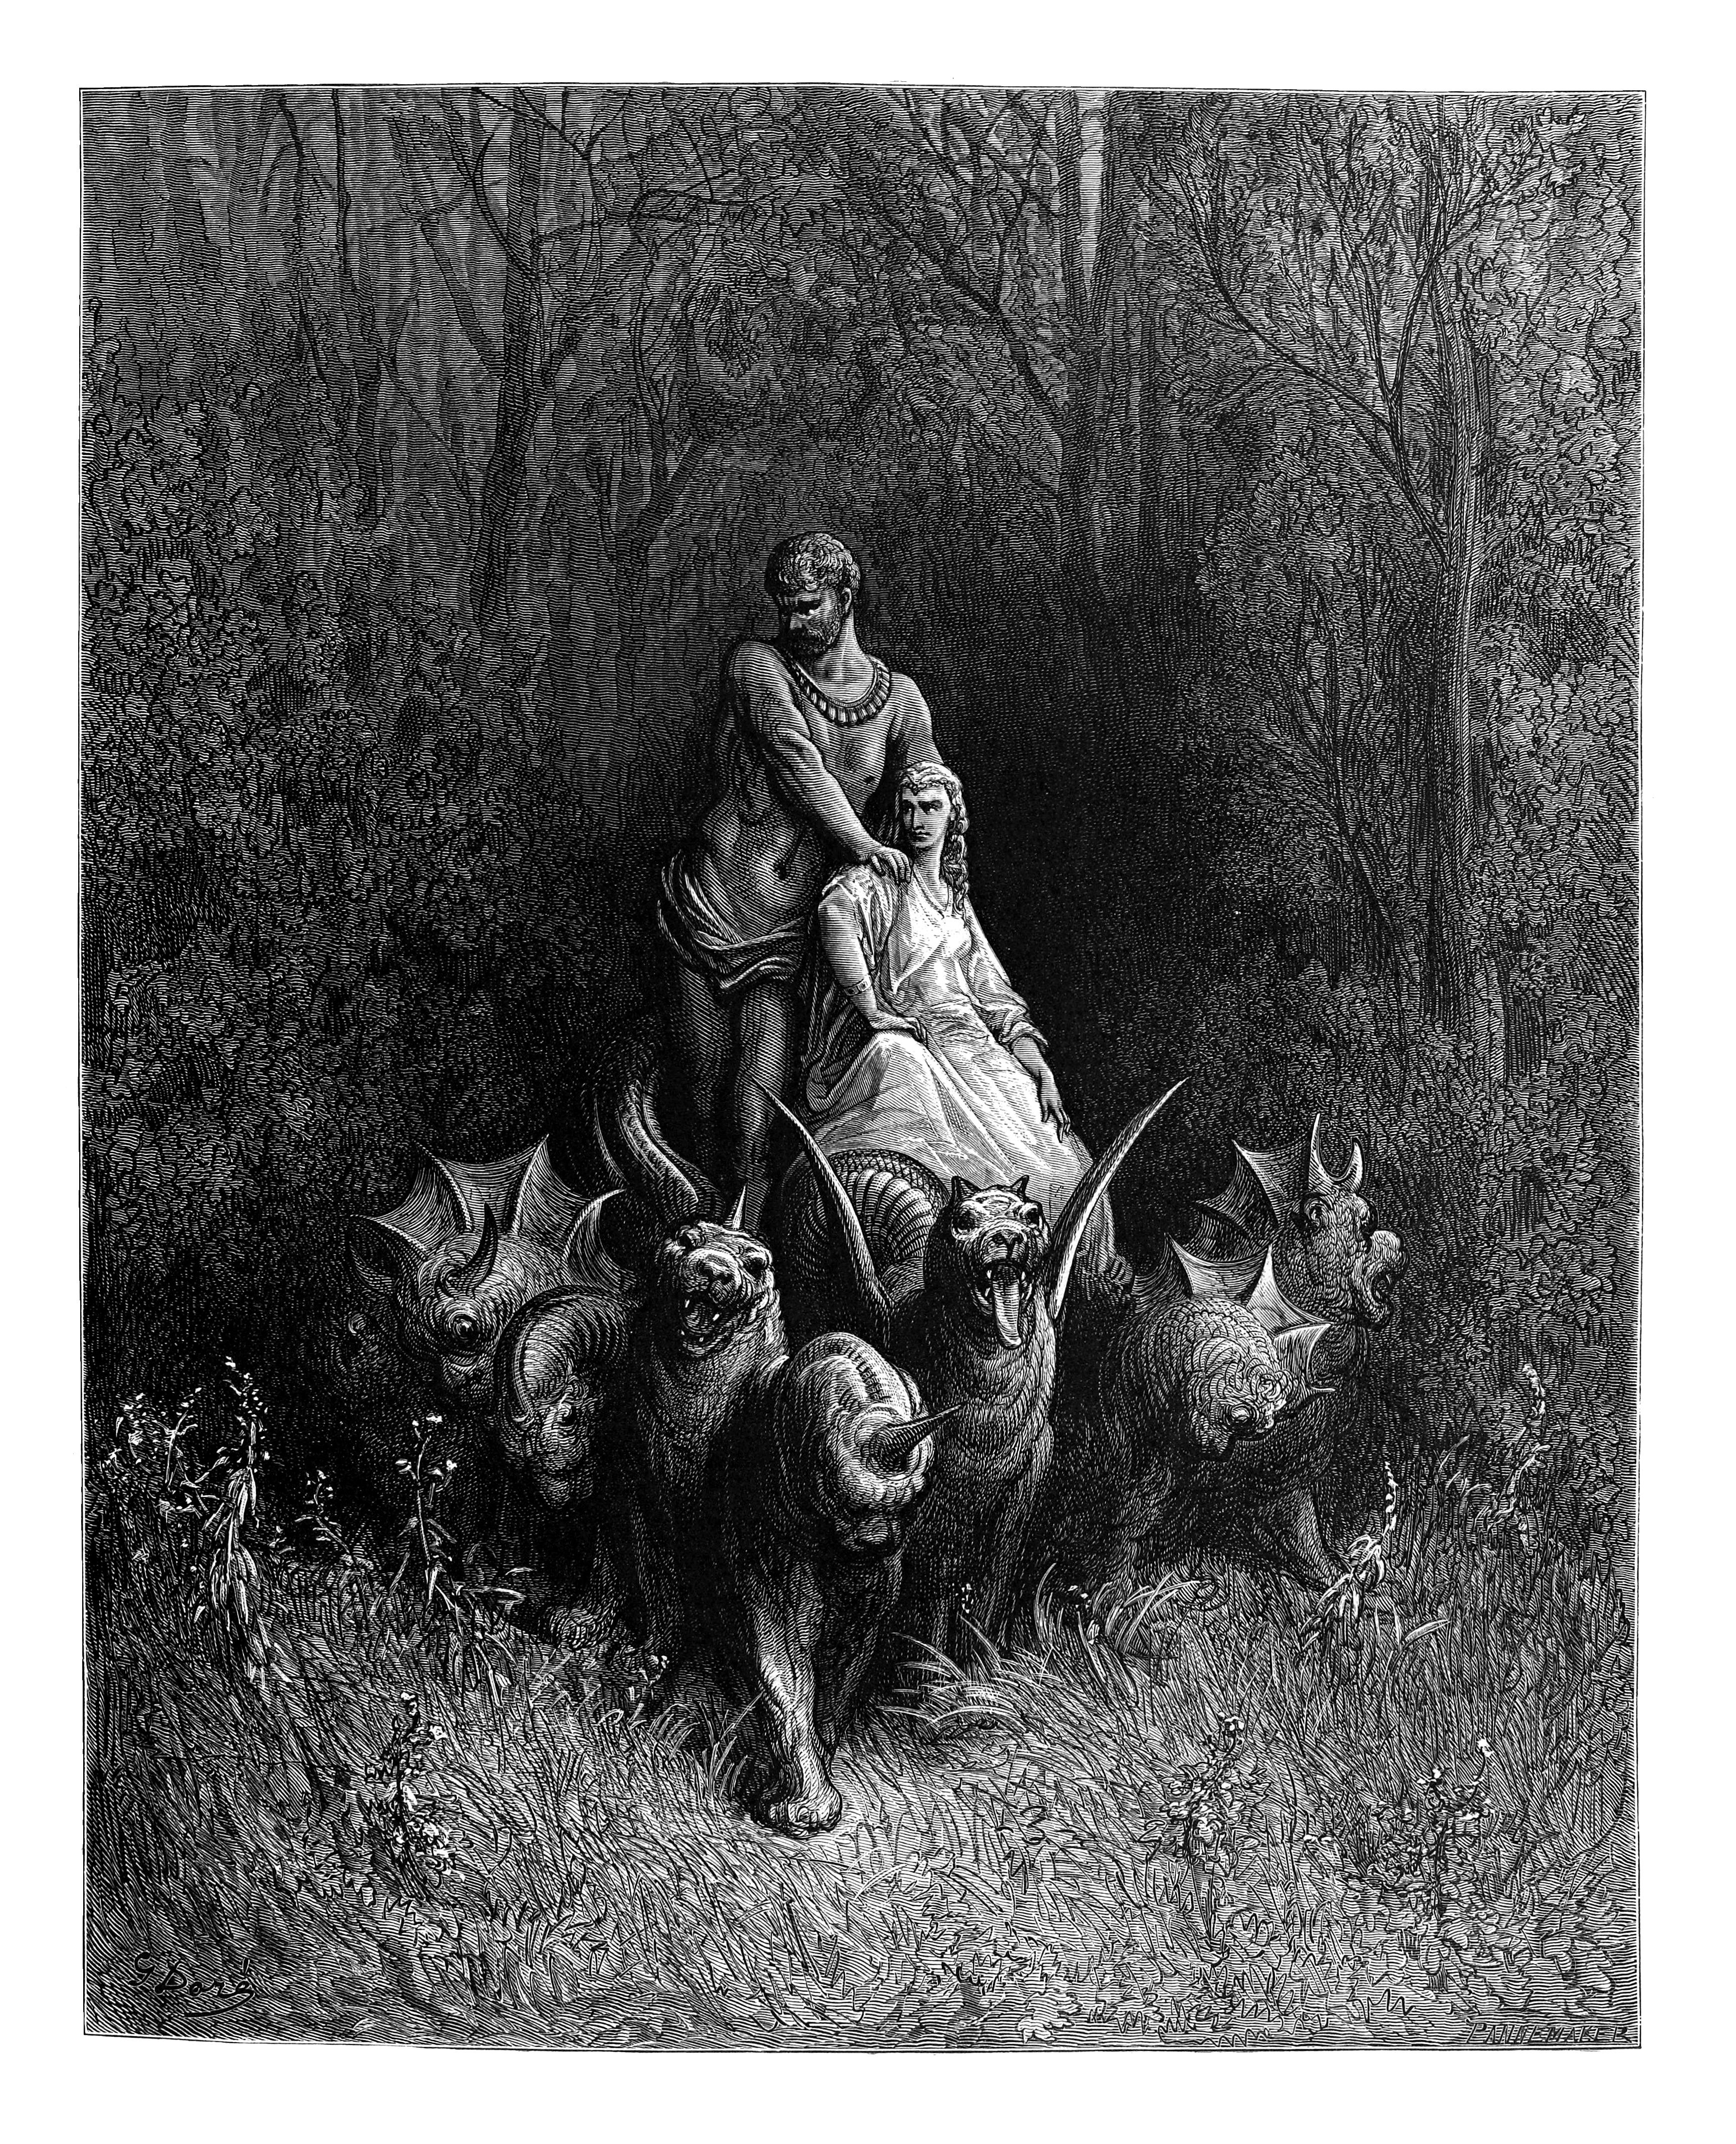
\includegraphics[height=\figsize]{illustrations/book_2/V02, c32.jpg}
\end{figure}

\begin{center}
\begin{minipage}{0.8\linewidth}
\textit{\\
"Sicura, quasi rocca in alto monte,\\seder sovresso una puttana sciolta\\m’apparve con le ciglia intorno pronte;"} \\
—V02, c32 \\~\\
\textit{"O'er it me thought there sat, secure as rock\\On mountain's lofty top, a shameless whore,\\Whose ken rov'd loosely round her. …"} \\
—B02, c32
\end{minipage}
\end{center}

\newpage

\section{Canto 33}

\begin{figure}[ht]
\centering
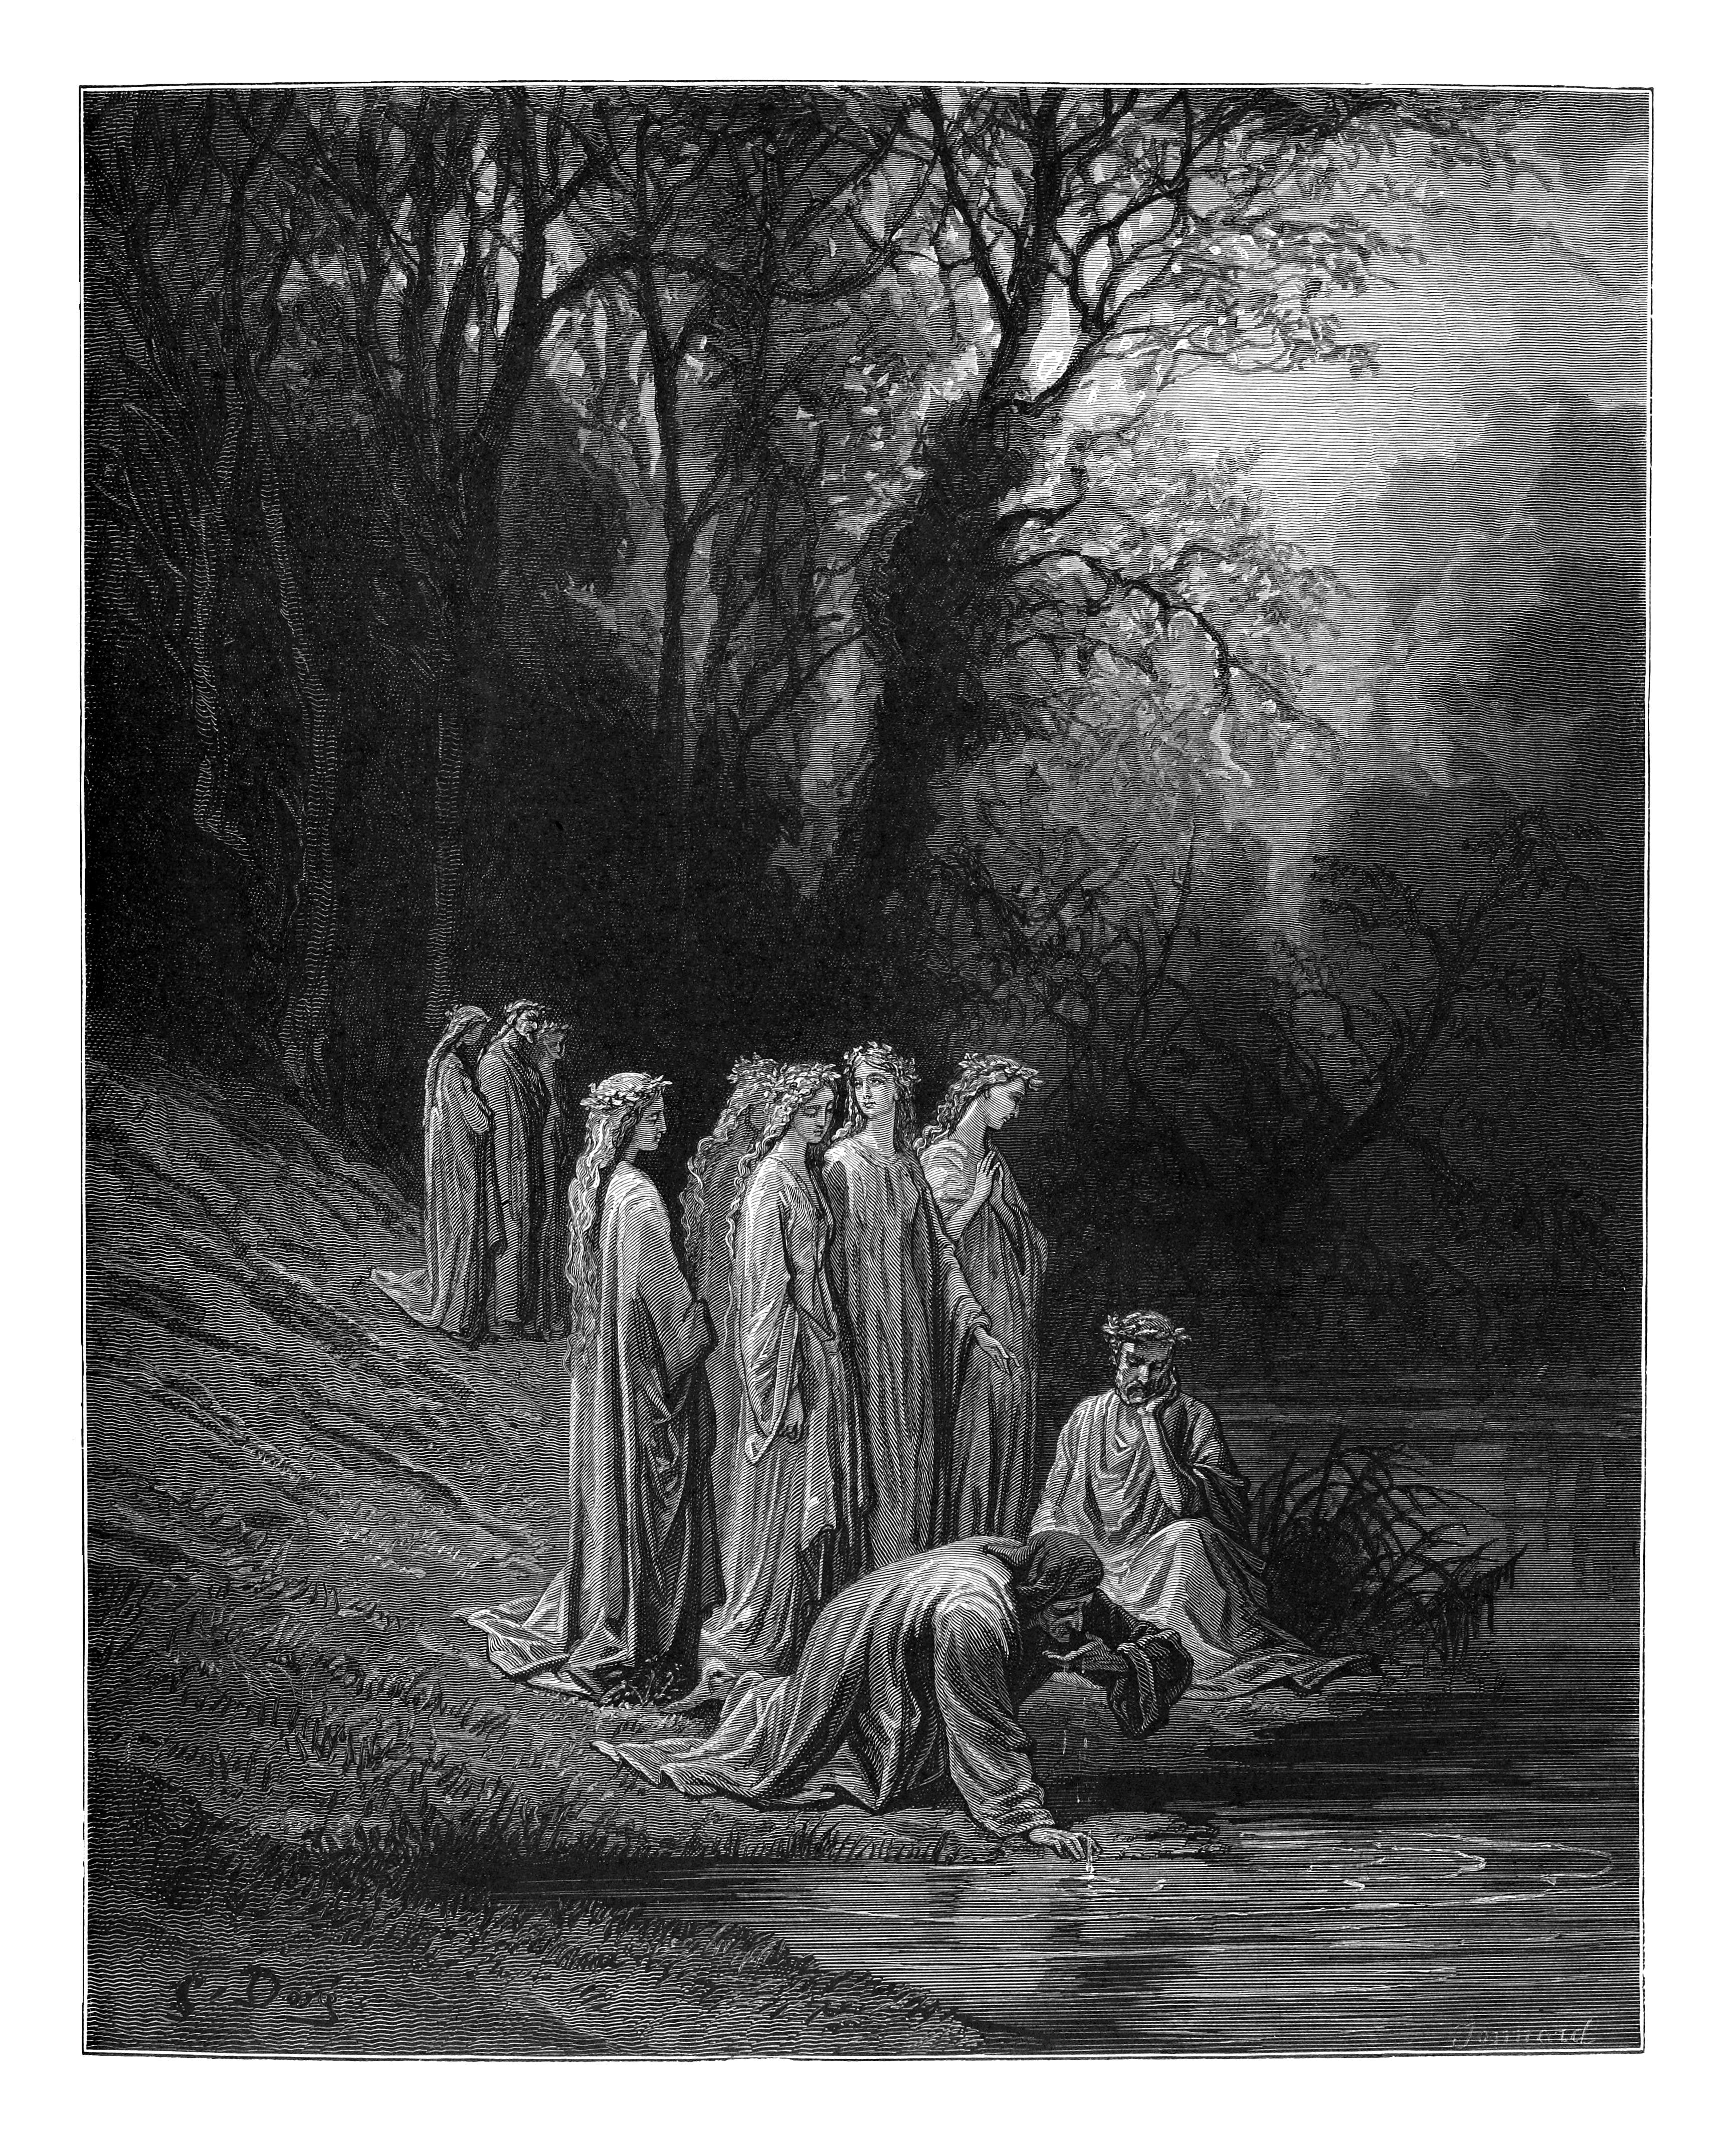
\includegraphics[height=\figsize]{illustrations/book_2/V02, c33.jpg}
\end{figure}

\begin{center}
\begin{minipage}{0.8\linewidth}
\textit{\\
"Io ritornai da la santissima onda\\rifatto s\`{\i} come piante novelle\\rinnovellate di novella fronda,\\puro e disposto a salire alle stelle."} \\
—V02, c33 \\~\\
\textit{"I return'd\\From the most holy wave, regenerate,\\If 'en as new plants renew'd with foliage new,\\Pure and made apt for mounting to the stars. …"} \\
—B02, c33
\end{minipage}
\end{center}

\end{document}